\documentclass{MScthesisITEM}

\usepackage{graphicx}
\usepackage{caption}
\usepackage{url}
\usepackage{hyperref}
\usepackage{glossaries}
\usepackage{listings}
\usepackage{color}
\usepackage{upquote}

\newcommand{\ttitle}{Unified Communication and WebRTC}
\newcommand{\subjectname}{Telematics}
\newcommand{\authorname}{Xiao Chen}
\newcommand{\tprofessor}{Mazen Malek Shiaa, ITEM}
\newcommand{\keywordnames}{WebRTC, AngularJs, Nodejs, SIP, WebSocket, Dialogic XMS}

% PDF meta-data
\hypersetup{pdftitle={\ttitle}}
\hypersetup{pdfsubject=\subjectname}
\hypersetup{pdfauthor=\authorname}
\hypersetup{pdfkeywords=\keywordnames}

%listings settings
\definecolor{editorGray}{rgb}{0.95, 0.95, 0.95}
\definecolor{editorOcher}{rgb}{1, 0.5, 0} % #FF7F00 -> rgb(239, 169, 0)
\definecolor{editorGreen}{rgb}{0, 0.5, 0} % #007C00 -> rgb(0, 124, 0)


\lstdefinelanguage{JavaScript}{
  morekeywords={typeof, new, true, false, catch, function, return, null, catch, switch, var, if, in, while, do, else, case, break},
  morecomment=[s]{/*}{*/},
  morecomment=[l]//,
  morestring=[b]",
  morestring=[b]'
}

\lstdefinelanguage{HTML5}{
        language=html,
        sensitive=true, 
        alsoletter={<>=-},
        otherkeywords={
        % HTML tags
        <html>, <head>, <title>, </title>, <meta, />, </head>, <body>,
        <canvas, \/canvas>, <script>, </script>, </body>, </html>, <!, html>, <style>, </style>, ><
        },  
        ndkeywords={
        % General
        =,
        % HTML attributes
        charset=, id=, width=, height=,
        % CSS properties
        border:, transform:, -moz-transform:, transition-duration:, transition-property:, transition-timing-function:
        },  
        morecomment=[s]{<!--}{-->},
        tag=[s]
}

\lstset{%
    % Basic design
    backgroundcolor=\color{editorGray},
    basicstyle={\small\ttfamily},   
    frame=l,
    % Line numbers
    xleftmargin={0.75cm},
    numbers=left,
    stepnumber=1,
    firstnumber=1,
    numberfirstline=true,
    % Code design   
    keywordstyle=\color{blue}\bfseries,
    commentstyle=\color{darkgray}\ttfamily,
    ndkeywordstyle=\color{editorGreen}\bfseries,
    stringstyle=\color{editorOcher},
    % Code
    language=HTML5,
    alsolanguage=JavaScript,
    alsodigit={.:;},
    tabsize=2,
    showtabs=false,
    showspaces=false,
    showstringspaces=false,
    extendedchars=true,
    breaklines=true,        
    % Support for German umlauts
    literate=%
    {Ö}{{\"O}}1
    {Ä}{{\"A}}1
    {Ü}{{\"U}}1
    {ß}{{\ss}}1
    {ü}{{\"u}}1
    {ä}{{\"a}}1
    {ö}{{\"o}}1
}

\renewcommand{\lstlistingname}{Code Snippet}% Listing -> Algorithm
\renewcommand{\lstlistlistingname}{List of \lstlistingname s}% List of Listings -> List of Algorithms

\title{\ttitle} % The title of your assignement; NB use \newlinetitle to start a newline
\author{\authorname} % Your firstname and lastname
\professor{\tprofessor} % Affiliation = ITEM for instance
\supervisor{\tprofessor}

%% Uncomment the following in case you want subfigures; note that there will be a warning for the caption package
% \let\subcaption\undefined
% \let\subfloat\undefined
% \usepackage[bf]{caption}
% \usepackage{subcaption}

\DeclareGraphicsExtensions{.pdf,.jpg,.png}
\graphicspath{{./figs/}}

\loadglsentries{glossary}
\makeglossaries

\begin{document}
\selectlanguage{english}
\pagenumbering{roman}
\pagestyle{plain}

%% Only for the project
\titleITEM

%% Only for the master's thesis; for the project report the description is taken from It's Learning and added by the department
\selectlanguage{english} % Change to 'norsk' if you are writing in Norwegian
\begin{titlingpage}

\noindent
\begin{tabular}{@{}p{4cm}l}
\textbf{Title:} 	& \thetitle \\
\textbf{Student:}	& \theauthor \\
\end{tabular}

\vspace{4ex}
\noindent\textbf{Problem description:}
\vspace{2ex}

\noindent \gls{webrtc} offers application developers the ability to write rich, real-time multimedia application (e.g. video chat) on the web, without requiring any plugins, downloads or installations. \gls{webrtc} is also currently the only existing soon-to-be standardized technology on the market to create horizontal cross-platform communication services, encompassing smartphones, tablets, PCs, laptops and TVs, which adds value for both consumers and enterprises. \gls{webrtc} gives operators the opportunity to offer telephony services to more devices, such as PCs, tablets and TVs.
This thesis considers how \gls{webrtc} can enhance the existing echo-systems for telephony and messaging services by providing the end-user rich application client.
\par It will also covers research about different solutions to implement \gls{webrtc} to cooperate with existing telephony services like hosted virtual \gls{pbx} services.
\par A prototype of \gls{webrtc} deployment based on different rich communication scenarios will be implemented along with this thesis. Some corresponding test and evaluation will be fulfilled in this prototype.
\par Research about advanced \gls{webrtc} usability in telephony and messaging services will be covered in this thesis by the feedback of the \gls{webrtc} prototype

\vspace{6ex}

\noindent
\begin{tabular}{@{}p{4cm}l}
\textbf{Responsible professor:} 	& \theprofessor \\
\textbf{Supervisor:}			& \thesupervisor \\
\end{tabular}

\end{titlingpage}
% \cleardoublepage

%% There must be an abstract in English, even though the main text is in Norwegian
\selectlanguage{english}
\pagestyle{empty}

\begin{abstract}
\noindent During the development of traditional telephony echo-systems, the cost of maintenaning traditional telephony network is getting higher and higher but the number of customer does not grow rapidly any more since almost every one has a phone to access the traditional telephony network. \gls{webrtc} is an \gls{api} definition drafted by the \gls{w3c} that supports browser-to-browser applications for voice calling, video chat, and \gls{p2p} file sharing without plugins.\cite{wiki:webRTC} “This technology, along with other advances in \gls{html5} browsers, has the potential to revolutionize the way we all communicate, in both personal and business spheres.”\cite{inbook:rtc-preface}
\par As network operators aspect, \gls{webrtc} provides many opportunities to the future telecommunication business module. To the users who have already had mobile service, operator can offer \gls{webrtc} service with session-based charging to the existing service plans. Messaging \gls{api}s can augment \gls{webrtc} web application with \gls{rcs} and other messaging services which developers have already implemented. Furthermore, since \gls{webrtc} is a web based \gls{api}, then the implementation of \gls{qos} for \gls{webrtc} can provide assurance to users and prioritize services (enterprise, emergency, law enforcement, eHealth) that a WebRTC service will work as well as they need it to. \gls{webrtc} almost provides network operator a complete new business market with a huge amount of new end-users.
\par As an end-user aspect, \gls{webrtc} provides a much simpler way to have real-time conversation with another end-user. It is based on browser and internet which almost personal or enterprise computer already have, without any installation and plugins, end-user can have exactly the same service which previous stand-alone desktop client provides. By the prototype system of this thesis will cover, the end-user can even have the real-time rich communication service with multiple kinds of end-users.
\par This thesis will cover the research about how to apply \gls{webrtc} technology with existing legacy \gls{voip} network.

\noindent \textbf{Keywords} : \keywordnames
\end{abstract}
% \cleardoublepage
\clearpage

%% Only for the master's thesis; if the main text is in English and you can write Norwegian, there must be an abstract in Norwegian as well.A
% \selectlanguage{norsk}
% \pagestyle{empty}
\renewcommand{\abstractname}{Sammendrag}
\begin{abstract}
\noindent Sikkerheten til nesten all offentlig nøkkel-kryptografi er basert på et vanskelig beregnbarhetsproblem. Mest velkjent er problemene med å faktorisere heltall i sine primtallsfaktorer, og å beregne diskrete logaritmer i endelige sykliske grupper. I de to siste tiårene, har det imidlertid dukket opp en rekke andre offentlig nøkkel-systemer, som baserer sin sikkerhet på helt andre type problemer. Et lovende forslag, er å basere sikkerheten på vanskeligheten av å løse store likningsett av flervariable polynomlikninger. En stor utfordring ved å designe slike offentlig nøkkel-systemer, er å integrere en effektiv ``falluke'' (trapdoor) inn i likningssettet. En ny tilnærming til dette problemet ble nylig foreslått av Gligoroski m.f., hvor de benytter konseptet om kvasigruppe-strengtransformasjoner (quasigroup string transformations). I denne masteroppgaven beskriver vi en metodikk for å identifisere sterke og svake nøkler i det nylig foreslåtte multivariable offentlig nøkkel-signatursystemet MQQ-SIG, som er basert på denne idéen.

Vi har gjennomført et stort antall eksperimenter, basert på Gröbner basis angrep, for å klassifisere de ulike parametrene som bestemmer nøklene i MQQ-SIG. Våre funn viser at det er store forskjeller i viktigheten av disse parametrene. Metodikken består i en klassifisering av de forskjellige parametrene i systemet, i tillegg til en innføring av konkrete kriterier for hvilke nøkler som bør velges. Videre, har vi identifisert et unødvendig krav i den originale spesifikasjonen, som krevde at kvasigruppene måtte oppfylle et bestemt kriterie. Ved å fjerne denne betingelsen, kan nøkkel-genererings-algoritmen potensielt øke ytelsen med en stor faktor. Basert på alt dette, foreslår vi en ny og forbedret nøkkel-genereringsalgoritme for MQQ-SIG, som vil generere sterkere nøkler og være mer effektiv enn den originale nøkkel-genereringsalgoritmen.  
\end{abstract}
% \cleardoublepage

\selectlanguage{english}% Change to 'norsk' if you are writing in Norwegian

\renewcommand{\abstractname}{Preface}
\begin{abstract}

\noindent \gls{webrtc} is quite popular topic in the web development filed since the massive usage and development of \gls{html5} web applications on the internet. The initial purpose of this web \gls{api} is to provide the browser client the ability to create real-time conversation between each other. After many \gls{webrtc} based application came out in the market, it is quite normal to think about how to integrate these kinds of web applications with the current legacy telephony network as the next big step for this technology. The requirement of this function is not only from the traditional telephony operator but also the normal end-users.

\par As network operators aspect, \gls{webrtc} provides many opportunities to the future telecommunication business module. For mobile phone customers, operator can offer \gls{webrtc} service with session-based charging to the existing service plans. Messaging \gls{api}s can augment \gls{webrtc} web application with \gls{rcs} and other messaging services which developers have already implemented. Furthermore, since \gls{webrtc} is a web based \gls{api}, then the implementation of \gls{qos} for \gls{webrtc} can provide assurance to users and prioritize services (enterprise, emergency, law enforcement, eHealth) that a WebRTC service will work as well as they need it to. \gls{webrtc} almost provides network operator a complete new business market with a huge amount of new end-users.

\par As an end-user aspect, \gls{webrtc} provides a much simpler way to have real-time conversation with another end-user. It is based on browser and internet which almost personal or enterprise computer already have, without any installation and plugins, end-user can have exactly the same service which previous stand-alone desktop client provides. By the prototype system of this thesis will cover, the end-user can even have the real-time rich communication service with multiple kinds of end-users.

\par The goal of this thesis and prototype system is to make an unified communication solution for \gls{ip} network and traditional telephony network by using\gls{webrtc}.

\end{abstract}
% \cleardoublepage
\clearpage

% similarly you may add a separate acknowledgments page
\renewcommand{\abstractname}{Acknowledgment}
\begin{abstract}
\vspace*{\fill}
 \begin{center}
	 	Written by Xiao Chen in Trondheim in May 2014

		Thanks for \tprofessor
		
		Frank Mbaabu Kiriinya, Gintel AS
		
		Roman Stobnicki, Dialogic, the Network Fuel company

		Special thanks for Gintel AS
		
		Source code of prototype system is owned by Xiao Chen and Gintel AS
		
 \end{center}
\vspace*{\fill}
\end{abstract}
\clearpage

\tableofcontents*
\clearpage

%% include if relevant
\listoffigures
\clearpage

%% include if relevant
\listoftables
\clearpage

%% include if relevant
\lstlistoflistings
\clearpage

%% include if relevant
\printglossary[title=List of Symbols, style=long]
\clearpage
\glsaddall[]

%% include if relevant
\printglossary[title=List of Acronyms,type=\acronymtype] % prints just the list of acronyms
\clearpage

\pagenumbering{arabic}
\pagestyle{ruled}

\chapter{Introduction}
\label{chp:intro}
\noindent In this Chapter, introduction of \gls{webrtc} and \gls{sip} network will be covered. \gls{sip} is one of the \gls{voip} signaling protocols widely used in current internet telephony service which is also the target telephony network integrated with \gls{webrtc} application system in this thesis.

\section{WebRTC}

\noindent Gmail\footnote{Gmail is a free , advertising-supported email service provided by Google.} video chat became popular in 2008, and in 2011 Google introduced Hangouts\footnote{Google Hangouts is an instant messaging and video chat platform developed by Google, which launched on May 15, 2013 during the keynote of its I/O development conference. It replaces three messaging products that Google had implemented concurrently within its services, including Talk, Google+ Messenger, and Hangouts, a video chat system present within Google+.}, which use the Google Talk service (as does Gmail). Google bought \gls{gips}, a company which had developed many components required for \gls{rtc}, such as codecs and echo cancellation techniques. Google open sourced the technologies developed by \gls{gips} and engaged with relevant standards bodies at the \gls{ietf} and \gls{w3c} to ensure industry consensus. In May 2011, Ericsson built the first implementation of \gls{webrtc}.

\subsection{What is WebRTC ?}

\noindent \gls{webrtc} is an industry and standards effort to put real-time communications capabilities into all browsers and make these capabilities accessible to web developers via standard \gls{html5} tags and JavaScript \gls{api}s. For example, consider functionality similar to that offered by Skype\footnote{Skype is a freemium voice-over-IP service and instant messaging client, currently developed by the Microsoft Skype Division.\cite{wiki:skype}}. but without having to install any software or plug-ins. For a website or web application to work regardless of which browser is used, standards are required. Also, standards are required so that browsers can communicate with non-browsers, including enterprise and service provider telephony and communications equipment\cite{inbook:rtc-intro}.

\par With the rapidly development of internet, more and more communication traffic is moving to web from the traditional telephony network. And in the recent decade, \gls{voip} network services are growing to the peek of the market capacity. Solution to integrate \gls{webrtc} and existing \gls{voip} network is the right approach the trend of the internet communication requirement.

\subsection{WebRTC Network Structure}

\noindent In the Figure\ref{fig:webrtc_network_finCandidate}\cite{html5rock:webrtc} showing how the \gls{ice} framework\footnote{ICE is a framework for connecting peers, such as two video chat clients.\cite{wiki:ice}} to find peer candidate through \gls{stun} server and its extension \gls{turn} server.

\begin{figure}
	\centering
    	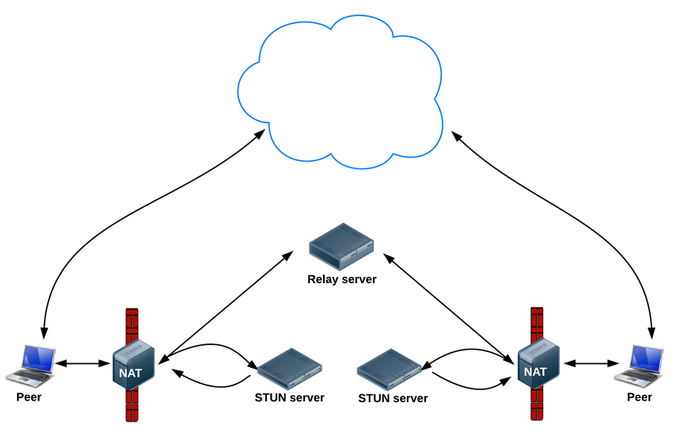
\includegraphics[height=0.30\textheight,natwidth=610,natheight=642]{figs/webrtc_network_finCandidate.png}
  	\caption{\gls{webrtc} Network: Finding connection candidates}
  	\label{fig:webrtc_network_finCandidate}
\end{figure} 

\begin{figure}
	\centering
    	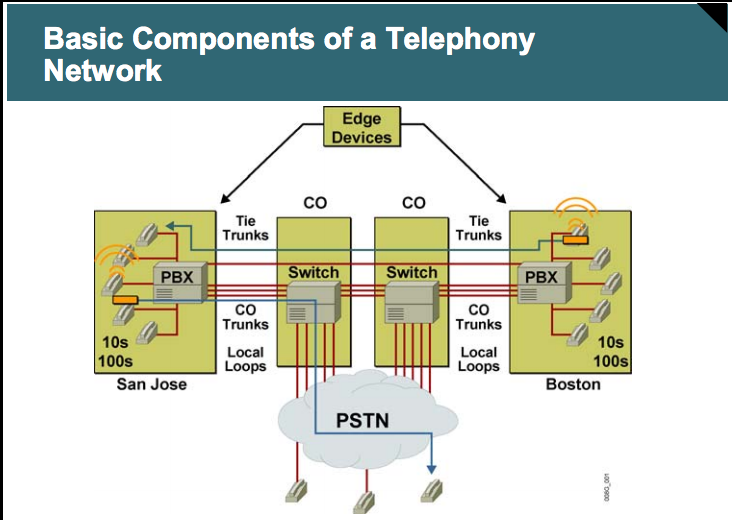
\includegraphics[height=0.40\textheight,natwidth=610,natheight=642]{figs/telephony_network.png}
  	\caption{Traditional Telephony Network}
  	\label{fig:telephony_network}
\end{figure}

\par Initially, \gls{ice} tries to connect peers directly, with the lowest possible latency, via \gls{udp}. In this process, \gls{stun} servers have a single task: to enable a peer behind a \gls{nat} to find out its public address and port. If \gls{udp} fails, \gls{ice} tries \gls{tcp}: first \gls{http}, then \gls{https}. If direct connection fails—in particular, because of enterprise \gls{nat} traversal and firewalls—\gls{ice} uses an intermediary (relay) \gls{turn} server. In other words, \gls{ice} will first use \gls{stun} with \gls{udp} to directly connect peers and, if that fails, will fall back to a \gls{turn} relay server. The expression 'finding candidates' refers to the process of finding network interfaces and ports.\cite{html5rock:webrtc}

\par The difference and usage of \gls{stun} server and \gls{turn} server will be discussed more detail in Chapter \ref{chp:sys_deploy}.

\par \gls{webrtc} needs server to help users discover each other and exchange 'real world' details such as names. Then \gls{webrtc} client applications (peers) exchange network information. After that, peers exchange data about media such as video format and resolution. Finally, \gls{webrtc} client applications can traverse \gls{nat} gateways and firewalls.

\par Compare to the traditional telephony network which is shown in Figure\ref{fig:telephony_network}\cite{web:teleVSvoip}, the main difference between these two communication network is that \gls{webrtc} is \gls{p2p} communication in \gls{stun} server scenario, after the signaling between end-peers, the media data are exchanged directly between tow peers. However, in the traditional telephony, all the media data are transferred to \gls{pbx} and switches regarding to \gls{pstn}\footnote{The PSTN consists of telephone lines, fiber optic cables, microwave transmission links, cellular networks, communications satellites, and undersea telephone cables, all interconnected by switching centers, thus allowing any telephone in the world to communicate with any other. Originally a network of fixed-line analog telephone systems, the PSTN is now almost entirely digital in its core network and includes mobile and other networks, as well as fixed telephones.\cite{wiki:pstn}} then reach the other side of the peer. Even in \gls{turn} server scenario for \gls{webrtc}, the media stream is only relaying to the \gls{turn} then directly transfer to another peer, no switches involved. Two server working scenario will be discussed in Chapter \ref{chp:sys_dev}.

\subsection{WebRTC Implementation Steps}

\begin{figure}
	\centering
    	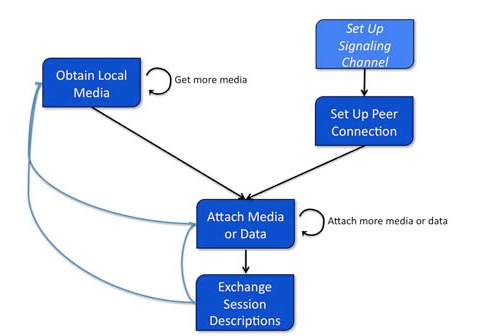
\includegraphics[width=0.80\textwidth,natwidth=610,natheight=642]{figs/webrtcApis.png}
  	\caption{WebRTC \gls{api} View with Signaling\cite{inbook:rtc-apis}}
  	\label{fig:webrtc_4steps}
\end{figure}

\noindent There are four main steps to implement a \gls{webrtc} session shown in Figure \ref{fig:webrtc_4steps}. The browser client need to obtain local media first, then set up a connection between the browser and the other peer through some signaling, after that attach the media and data channels to the connection, afterwards exchange the session description from each other. Finally the media stream will automatically exchange through the real-time peer to peer media channel.

\par Each step shown in the Figure \ref{fig:webrtc_4steps} is implemented by some \gls{webrtc} \gls{api}s. More detail about how to use \gls{webrtc} \gls{api}s to implement these steps will be covered in Chapter \ref{chp:sys_dev}. The \gls{webrtc} architecture is shown in Figure \ref{fig:webrtc_api_arch}, the main focus in this thesis will be Web \gls{api} part and transport part because Web \gls{api} is the tool to implement the \gls{webrtc} application and transport part is the key for \gls{webrtc} application to communicate with application server, media server and other end peer in the system. 

\begin{figure}
	\centering
    	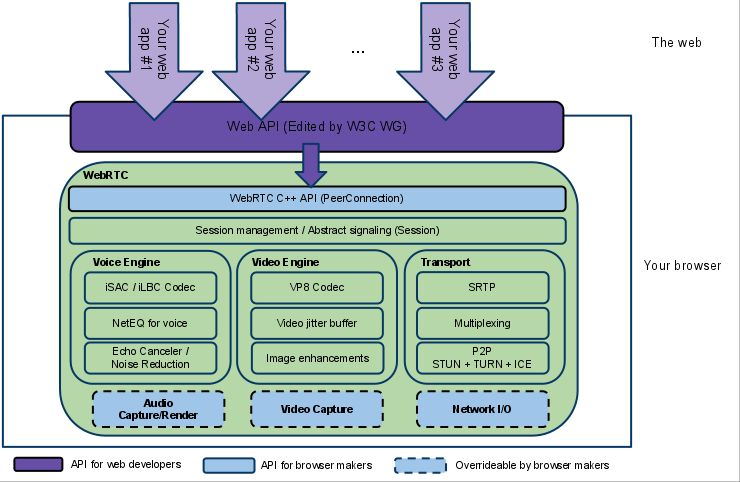
\includegraphics[width=0.80\textwidth,natwidth=610,natheight=642]{figs/WebRTCapiPic.png}
  	\caption{\gls{webrtc} architecture \cite{org:webrtc}}
  	\label{fig:webrtc_api_arch}
\end{figure}

\par Besides \gls{webrtc} \gls{api}s, signaling is the other important factor in the system. \gls{webrtc} uses \textit{RTCPeerConnection} (more about this \gls{api} will be discussed in Chapter \ref{chp:sys_dev}) to communicate streaming data between browsers, but also needs a mechanism to coordinate communication and to send control messages, a process known as signaling. Signaling methods and protocols are not specified by \gls{webrtc} by Google purpose, so signaling is not part of the \textit{RTCPeerConnection} \gls{api}.

\par Instead, \gls{webrtc} app developers can choose whatever messaging protocol they prefer, such as \gls{sip} or \gls{xmpp}, and any appropriate duplex (two-way) communication channel. The prototype application in this thesis will use WebSocket\footnote{WebSocket is a protocol providing full-duplex communications channels over a single TCP connection.\cite{wiki:websocket}} as signaling between \gls{webrtc} browser end point and keep use \gls{sip} as signaling for \gls{sip} end point (mobile/fixed phone based on \gls{pstn} in this case).

\noindent Signaling is used to exchange three types of information\cite{html5rock:webrtc}:

\begin{itemize}[topsep=-1em,parsep=0em,itemsep=0em]
 \item Session control messages: to initialize or close communication and report errors.
 \item Network configuration: to the outside world, the computer's IP address and port.
 \item Media capabilities: the codecs and resolutions can be handled by the browser and the browser it wants to communicate with.
\end{itemize}

\par The exchange of information via signaling must have completed successfully before peer-to-peer streaming can begin. For the prototype application in this thesis, the signaling has two mechanisms, one is for \gls{webrtc} browser clients and the other is for \gls{sip} clients, it will be explained in Chapter \ref{chp:sys_dev}.

\section{SIP}
\noindent The prototype application in this thesis will be integrated with \gls{pstn} through \gls{sip} server. Therefore the application server implemented in this system will use \gls{sip} signaling to communicate with \gls{sip} server to handle the signaling configuration with mobile/fixed phone end-point.

\subsection{What is SIP?}
\noindent The \gls{sip} is a signaling communications protocol, widely used for controlling multimedia communication sessions such as voice and video calls over \gls{ip} networks.

\par The protocol defines the messages that are sent between endpoints which govern establishment, termination and other essential elements of a call. \gls{sip} can be used for creating, modifying and terminating sessions consisting of one or several media streams. \gls{sip} can be used for two-party (unicast) or multiparty (multicast) sessions. Other \gls{sip} applications include video conferencing, streaming multimedia distribution, instant messaging, presence information, file transfer, fax over \gls{ip} and online games.\cite{wiki:sip}

\par \gls{sip} works in conjunction with several other application layer protocols that identify and carry the session media. Media identification and negotiation is achieved with the \gls{sdp}. It is different key filed format than the \gls{webrtc} \gls{sdp}. For the transmission of media streams (voice, video) \gls{sdp} typically employs the \gls{rtp} or \gls{srtp}. For secure transmissions of \gls{sip} messages, the protocol may be encrypted with \gls{tls}.

\subsection{SIP Network Elements}
\noindent In normal \gls{sip} network, \gls{sip} defines user-agents as well as several types of server network elements. Two \gls{sip} endpoints can communicate without any intervening \gls{sip} infrastructure. However, this approach is often impractical for a public service, which needs directory services to locate available nodes on the network. In the system implemented of this thesis, the application server will play as 'User Agent', 'Registrar' and 'Gateway' elements in the network.

\noindent \textbf{User Agent}\cite{wiki:sip}:
\par A \gls{sip} \gls{ua} is a logical network end-point used to create or receive \gls{sip} messages and thereby manage a \gls{sip} session. A \gls{sip} \gls{ua} can perform the role of a \gls{uac}, which sends \gls{sip} requests, and the \gls{uas}, which receives the requests and returns a \gls{sip} response. These roles of \gls{uac} and \gls{uas} only last for the duration of a \gls{sip} transaction.

\noindent \textbf{Registrar}\cite{wiki:sip}:
\par A registrar is a \gls{sip} endpoint that accepts REGISTER requests and places the information it receives in those requests into a location service for the domain it handles. The location service links one or more \gls{ip} addresses to the \gls{sip} \gls{uri} of the registering agent. The \gls{uri} uses the sip: scheme, although other protocol schemes are possible, such as tel:. More than one user agent can register at the same \gls{uri}, with the result that all registered user agents receive the calls to the \gls{uri}.

\noindent \textbf{Gateway}\cite{wiki:sip}:
\par Gateways can be used to interface a \gls{sip} network to other networks, such as the \gls{pstn}, which use different protocols or technologies. In the prototype application, the application server is the gateway to interface a \gls{webrtc} WebSocket network (The working process will be covered in Chapter \ref{chp:sys_dev}).

\subsection{SIP messages}
\noindent Since the application server in this system will be used as \gls{sip} \gls{ua} and \gls{sip} Gateway, it will send \gls{sip} message request to \gls{sip} server and receive \gls{sip} message request from the \gls{sip} server.

\par One of the wonderful things about \gls{sip} is that it is a text-based protocol modeled on the request/response model used in HTTP.  This makes it easy to debug because the messages are easy to construct and easy to see.  Contrasted with H.323\footnote{H.323 is a recommendation from the ITU Telecommunication Standardization Sector (ITU-T) that defines the protocols to provide audio-visual communication sessions on any packet network. The H.323 standard addresses call signaling and control, multimedia transport and control, and bandwidth control for point-to-point and multi-point conferences.\cite{wiki:h323}}, SIP is an exceedingly simple protocol.  Nevertheless, it has enough powerful features to model the behavior of a very complex traditional telephone \gls{pbx}.\cite{networkworld:sip}

\par There are two different types of \gls{sip} messages: requests and responses. The first line of a request has a method, defining the nature of the request, and a Request-URI, indicating where the request should be sent.The first line of a response has a response code.

\noindent For sip requests, regarding to RFC 3261\cite{rfc:3261}, the application server in the system will use following \gls{sip} messages:

\begin{itemize}[topsep=-1em,parsep=0em,itemsep=0em]
 \item \textbf{REGISTER:} Used by a \gls{ua} to indicate its current \gls{ip} address and the \gls{url}s for which it would like to receive calls.
 \item \textbf{INVITE:} Used to establish a media session between user agents.
 \item \textbf{ACK:} Confirms reliable message exchanges.
 \item \textbf{CANCEL:} Terminates a pending request.
 \item \textbf{BYE:} Terminates a session between two users in a conference.
\end{itemize}

\noindent The \gls{sip} response types defined in RFC 3261 will be listened by application server in the following response codes\cite{wiki:sip_response_codes}:

\begin{itemize}[topsep=-1em,parsep=0em,itemsep=0em]
 \item \textbf{100 Trying:} Extended search being performed may take a significant time so a forking proxy must send a 100 Trying response.
 \item \textbf{180 Ringing:} Destination user agent received INVITE, and is alerting user of call.
 \item \textbf{200 OK:} Indicates the request was successful.
 \item \textbf{400 Bad Request:} The request could not be understood due to malformed syntax.
 \item \textbf{401 Unauthorized:} The request requires user authentication. This response is issued by \gls{uas}s and registrars.
 \item \textbf{408 Request Timeout:} Couldn't find the user in time. The server could not produce a response within a suitable amount of time, for example, if it could not determine the location of the user in time. The client MAY repeat the request without modifications at any later time.
 \item \textbf{480 Temporarily Unavailable:} Callee currently unavailable.
 \item \textbf{486 Busy Here:} Callee is busy.
\end{itemize}

\par By listening these \gls{sip} response, the application will send request to either \gls{webrtc} browser client or \gls{sip} client to play as the gateway role in the system. This gateway mechanism will be introduced in Chapter \ref{chp:sys_dev}.

\section{Prototype System Working Flow}
\noindent The main purpose of this thesis is to make unified communication solution with \gls{webrtc} technology. 
\par To connect with the traditional telephony network, the \gls{voip} system bridges the \gls{pstn} and the \gls{ip} network. \gls{voip} systems employ session control and signaling protocols to control the signaling, set-up, and tear-down of calls. They transport audio streams over \gls{ip} networks using special media delivery protocols that encode voice, audio, video with audio codecs, and video codecs as Digital audio by streaming media. In this prototype, \gls{sip} signaling is used because of its widely usage and current target \gls{pstn} has \gls{sip} server support.

\begin{figure}
	\centering
    	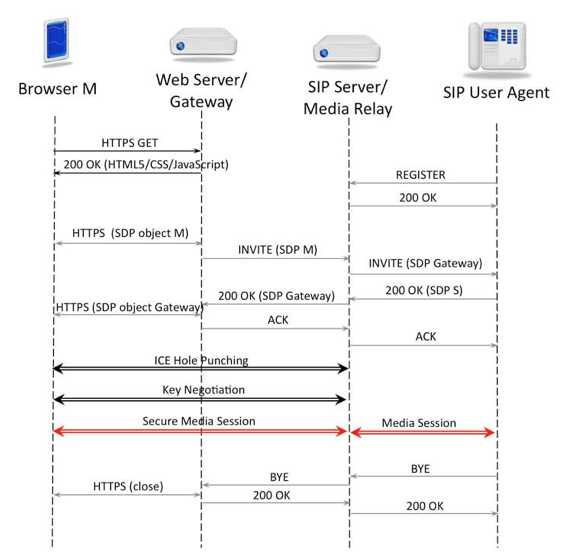
\includegraphics[width=0.60\textheight,natwidth=610,natheight=642]{figs/system_work_flow.png}
  	\caption{Prototype System Working Diagram \cite{inbook:sys_work_diagram}}
  	\label{fig:sys_work_diagram}
\end{figure}

\par The Figure \ref{fig:sys_work_diagram} shows the basic working flow of the prototype system. The Web Server is the application server in the system, it mainly bridges the \gls{webrtc} browser client with other \gls{webrtc} clients and the \gls{sip} network. The \gls{sip} server bridges the \gls{sip} network and \gls{pstn} network or traditional telephony network. And also the Media Relay server relay all the media stream from different end clients, in the prototype system, it is a media server provided by Dialogic, the Network Fuel company, which is called PowerMedia XMS v2.1\footnote{PowerMedia XMS is pre-integrated with a variety of application servers and signaling gateways with HTTP-to-SIP (H2S) functionality and rapidly integrates with others using its web API or standard interfaces.} PowerMedia XMS acts as a WebRTC Media Gateway to mediate WebRTC media-plane differences from those of typical existing VoIP networks including encryption interworking, transcoding, and client-based NAT traversal support. The reason to use this media server is to avoid hard-code transition between \gls{webrtc} \gls{sdp} and \gls{sip} \gls{sdp}. Then the end client no matter it is \gls{webrtc} client or \gls{sip} client, they will communicate with the same signaling client for their aspect.
\par Moreover, since the media server is used in this case, during the multiple end-point conversation, each end-point will only exchange their media stream to the single end-point on the media server (PowerMedia XMS server), it will make light client and centralized server control. The benefit of this system architecture will be discussed more in the Chapter \ref{chp:sys_dev}.

\par Therefore, in the Figure \ref{fig:sys_work_diagram}, all the end point keep using their own original signaling protocol to communicate with different server in order to reach different scope end point.
\chapter{Related Studies}
\label{chp:pre_study}

\noindent In order to bridge the \gls{ip} network and telephony network, a solution to create a real-time communication channel between \gls{ip} network and \gls{voip} network is the key factor since the \gls{voip} network is the bridge to make \gls{ip} network to talk with telephony network. In this Chapter, some introduction of \gls{webrtc} and \gls{sip} network will be covered. \gls{sip} is one of the \gls{voip} signaling protocols widely used in current internet telephony service which is also the target telephony network in this thesis. There will be some studies of \gls{webrtc} business cases and prototype working scenario based on these \gls{webrtc} usage cases in this chapter. The prototype working scenario is designed by considering these different \gls{webrtc} usage cases.

\section{WebRTC}

\noindent Before \gls{webrtc} announced, Gmail\footnote{Gmail is a free , advertising-supported email service provided by Google.} video chat became popular in 2008, and in 2011 Google introduced Hangouts\footnote{Google Hangouts is an instant messaging and video chat platform developed by Google, which launched on May 15, 2013 during the keynote of its I/O development conference. It replaces three messaging products that Google had implemented concurrently within its services, including Talk, Google+ Messenger, and Hangouts, a video chat system present within Google+.}, which uses the Google Talk service (as does Gmail). In May 2011, Google released an open source project for browser-based real-time communication known as \gls{webrtc}. This has been followed by ongoing work to standardize the relevant protocols in the \gls{ietf} and browser \gls{api}s in the \gls{w3c}.

\subsection{What is WebRTC ?}

\noindent \gls{webrtc} is an industry and standards effort to put real-time communications capabilities into all browsers and make these capabilities accessible to web developers via standard \gls{html5} tags and JavaScript \gls{api}s. For example, consider functionality similar to that offered by Skype\footnote{Skype is a freemium voice-over-IP service and instant messaging client, currently developed by the Microsoft Skype Division.\cite{wiki:skype}}. but without installing any software or plug-ins. For a website or web application to work regardless of which browser is used, standards are required. Also, standards are required so that browsers can communicate with non-browsers, including enterprise and service provider telephony and communications equipment\cite{inbook:rtc-intro}.

\par With the rapidly development of internet, more and more communication traffic is moving to web from the traditional telephony network. And in the recent decade, \gls{voip} network services are growing to the peek of the market capacity. Solution to integrate \gls{webrtc} and existing \gls{voip} network is the right approach the trend of the internet communication requirement.

\subsection{WebRTC Network Structure}

\noindent In the Figure\ref{fig:webrtc_network_finCandidate}\cite{html5rock:webrtc} shows how the \gls{ice} framework\footnote{ICE is a framework for connecting peers, such as two video chat clients.\cite{wiki:ice}} to find peer candidate through \gls{stun} server and its extension \gls{turn} server.

\begin{figure}
	\centering
    	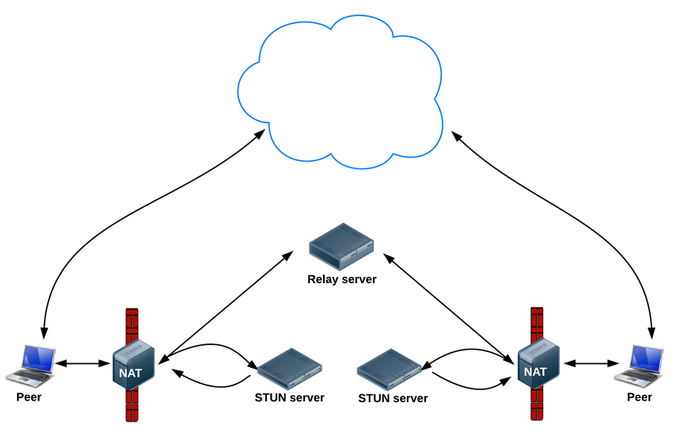
\includegraphics[height=0.30\textheight,natwidth=610,natheight=642]{figs/webrtc_network_finCandidate.png}
  	\caption{\gls{webrtc} Network: Finding connection candidates\cite{html5rock:webrtc}}
  	\label{fig:webrtc_network_finCandidate}
\end{figure} 

\begin{figure}
	\centering
    	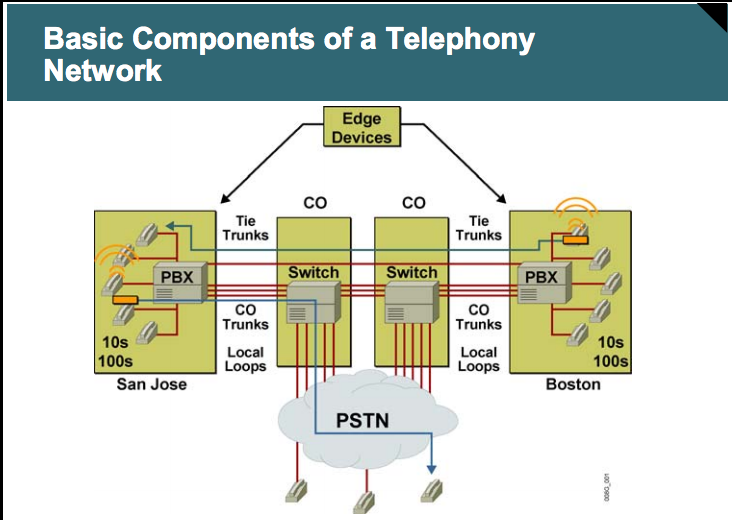
\includegraphics[height=0.40\textheight,natwidth=610,natheight=642]{figs/telephony_network.png}
  	\caption{Traditional Telephony Network}
  	\label{fig:telephony_network}
\end{figure}

\par Initially, \gls{ice} tries to connect peers directly, with the lowest possible latency, via \gls{udp}. In this process, \gls{stun} servers have a single task which is to enable a peer behind a \gls{nat} to find out its public address and port. If \gls{udp} fails, \gls{ice} tries \gls{tcp} (first \gls{http}, then \gls{https}). If direct connection fails in particular, because of enterprise \gls{nat} traversal and firewalls \gls{ice} uses an intermediary (relay) \gls{turn} server. In other words, \gls{ice} will first use \gls{stun} with \gls{udp} to directly connect peers and, if that fails, will fall back to a \gls{turn} relay server. The expression 'finding candidates' refers to the process of finding network interfaces and ports.\cite{html5rock:webrtc}

\par The difference and usage of \gls{stun} server and \gls{turn} server will be discussed more detail in Chapter \ref{chp:sys_deploy}.

\par \gls{webrtc} needs server to help users discover each other and exchange 'real world' details such as names. Then \gls{webrtc} client applications (peers) exchange network information. After that, peers exchange data information about media such as video format and resolution. Finally, \gls{webrtc} client applications can traverse \gls{nat} gateways and firewalls.

\par Compare to the traditional telephony network which is shown in Figure\ref{fig:telephony_network}\cite{web:teleVSvoip}, the main difference between these two communication network is that \gls{webrtc} is \gls{p2p} communication in \gls{stun} server scenario, after the signaling between end-peers, the media data are exchanged directly between two peers. However, in the traditional telephony, all the media data are transferred to \gls{pbx} and switches regarding to \gls{pstn}\footnote{The PSTN consists of telephone lines, fiber optic cables, microwave transmission links, cellular networks, communications satellites, and undersea telephone cables, all interconnected by switching centers, thus allowing any telephone in the world to communicate with any other. Originally a network of fixed-line analog telephone systems, the PSTN is now almost entirely digital in its core network and includes mobile and other networks, as well as fixed telephones.\cite{wiki:pstn}} then reach the other side of the peer. Even in \gls{turn} server scenario for \gls{webrtc}, the media stream is only relaying to the \gls{turn} then directly transfer to another peer, no switches involved.

\subsection{WebRTC Implementation Steps}

\begin{figure}
	\centering
    	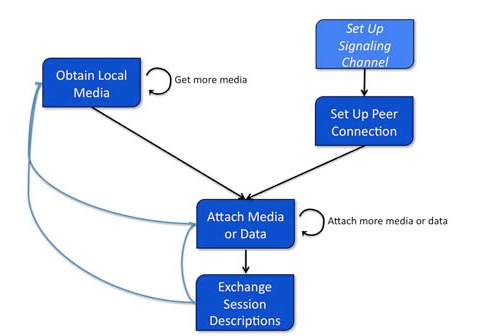
\includegraphics[width=0.80\textwidth,natwidth=610,natheight=642]{figs/webrtcApis.png}
  	\caption{WebRTC \gls{api} View with Signaling\cite{inbook:rtc-apis}}
  	\label{fig:webrtc_4steps}
\end{figure}

\noindent There are four main steps to implement a \gls{webrtc} session shown in Figure \ref{fig:webrtc_4steps}. The browser client need to obtain local media first, then set up a connection between the browser and the other peer through some signaling, after that attach the media and data channels to the connection, afterwards exchange the session description from each other. Then the media stream will automatically exchange through the real-time peer to peer media channel.

\par Each step shown in the Figure \ref{fig:webrtc_4steps} is implemented by some \gls{webrtc} \gls{api}s. More detail about how to use these \gls{webrtc} \gls{api}s to implement these steps will be covered in Chapter \ref{chp:sys_imp}. The \gls{webrtc} architecture is shown in Figure \ref{fig:webrtc_api_arch}, the main focus in this thesis will be Web \gls{api} part and transport part because Web \gls{api} is the tool to implement the \gls{webrtc} application and transport part is the key for \gls{webrtc} application to communicate with application server, media server and any other end peer in the system. 

\begin{figure}
	\centering
    	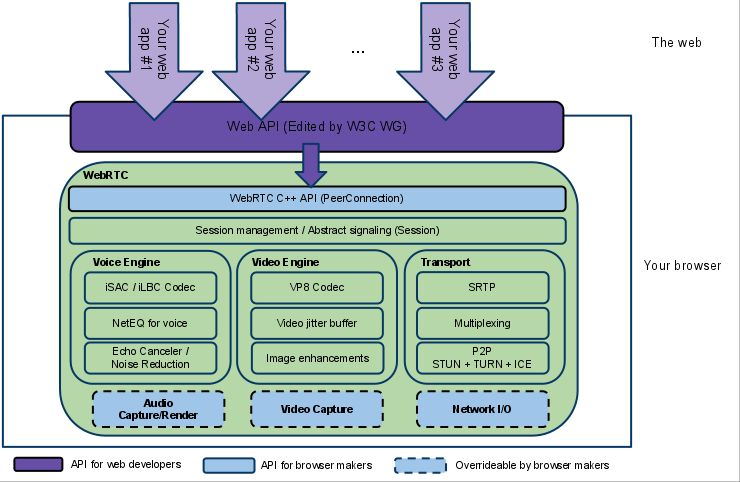
\includegraphics[width=0.80\textwidth,natwidth=610,natheight=642]{figs/WebRTCapiPic.png}
  	\caption{\gls{webrtc} architecture \cite{org:webrtc}}
  	\label{fig:webrtc_api_arch}
\end{figure}

\par Besides \gls{webrtc} \gls{api}s, signaling is the other important factor in the system. \gls{webrtc} uses \textit{RTCPeerConnection} (more about this \gls{api} will be discussed in Chapter \ref{chp:sys_imp}) to communicate streaming data between browsers, but also needs a mechanism to coordinate communication and to send control messages, a process known as signaling. Signaling methods and protocols are not specified by \gls{webrtc} by Google in purpose, then signaling is not part of the \textit{RTCPeerConnection} \gls{api} which can be decide how to implemented based on different project scenario.

\par Instead, \gls{webrtc} app developers can choose whatever messaging protocol they prefer, such as \gls{sip} or \gls{xmpp}, and any appropriate duplex (two-way) communication channel. The prototype application in this thesis will use WebSocket\footnote{WebSocket is a protocol providing full-duplex communications channels over a single TCP connection.\cite{wiki:websocket}} as signaling between \gls{webrtc} browser end point and keep use \gls{sip} as signaling for \gls{sip} end point (mobile/fixed phone based on \gls{pstn} in this case).

\noindent Signaling is used to exchange three types of information in \gls{webrtc}\cite{html5rock:webrtc}:

\begin{itemize}[topsep=-1em,parsep=0em,itemsep=0em]
 \item Session control messages: to initialize or close communication and report errors.
 \item Network configuration: to the outside world, the computer's IP address and port.
 \item Media capabilities: the codecs and resolutions can be handled by the browser and the browser it wants to communicate with.
\end{itemize}

\par The exchange of information via signaling must have completed successfully before peer-to-peer streaming can begin. For the prototype application in this thesis, the signaling has two mechanisms, one is for \gls{webrtc} browser clients and the other is for \gls{sip} clients, it will be explained in Chapter \ref{chp:sys_imp}.

\section{WebRTC Usage Cases}

\noindent After Google released the \gls{webrtc} as open source project. There are more and more web applications using it in different ways. \gls{webrtc} \gls{api}s includes three important \gls{api}s, shown below. There are mainly two types of the \gls{webrtc} applications used them in separately or cooperatively way.

\begin{itemize}[topsep=-1em,parsep=0em,itemsep=0em]
 \item \textbf{RTCPeerConnection:} audio or video calling, with facilities for encryption and bandwidth management.
  \item \textbf{MediaStream:} get access to data streams, such as from the user's camera and microphone.
 \item \textbf{RTCDataChannel:} peer-to-peer communication of generic data.
\end{itemize}

\par \textit{RTCPeerConnection} is the foundation of all \gls{webrtc} application to establish the peer to peer connection. For showing remote peer media source content and exchange the local peer media source content, the web application need to get the user's camera view and microphone sound, the \textit{MediaStream} \gls{api} is used always in real-time communication application. The following business usage cases, 'Tropo' and 'Uberconference', are in this category.

\subsection{Tropo}

\par Tropo is an application platform that enables web developers to write communication applications in the languages they already use, Groovy\footnote{Groovy is an object-oriented programming language for the Java platform. It is a dynamic language with features similar to those of Python, Ruby, Perl, and Smalltalk.\cite{wiki:groovy}}, Ruby\footnote{Ruby is a dynamic, reflective, object-oriented, general-purpose programming language. It was designed and developed in the mid-1990s by Yukihiro "Matz" Matsumoto in Japan.\cite{wiki:ruby}}, \gls{php}\footnote{PHP is a server-side scripting language designed for web development but also used as a general-purpose programming language.\cite{wiki:php}}, Python\footnote{Python is a widely used general-purpose, high-level programming language.\cite{wiki:python}} and JavaScript\footnote{JavaScript (JS) is a dynamic computer programming language.\cite{wiki:js}}, or use a Web \gls{api} which will talk with an application running on your own server through the use of \gls{http} and \gls{json}, feeding requests and processing responses back and forth as needed. Tropo is in the cloud, so it manages the headaches of dealing with infrastructure and keeping applications up and running at enterprise-grade. With Tropo, developers can build and deploy voice and telephony applications, or add voice to existing applications.\cite{web:tropo}

\par It has some advanced features, like 'Phone numbers around the world', 'Text messaging', 'Transcription', 'Call Recording', 'Conferencing', 'Text to Speech' and 'Speech Recognition'. The prototype system in this thesis will provide similar functions like 'Text messaging' and 'Conferencing'. Since Tropo is a cloud application platform, it generates its own scripts based on programming language to provide developer possibility to easily use \gls{webrtc} to communicate with other kinds of network rather than \gls{ip} network. The functions Tropo provided is implemented in application server in the prototype, the application server will handle both the \gls{sip} stack and \gls{webrtc} stack in the system. For the client, scripts will be host on the same application server for browser to access and use.

\subsection{Uberconference}

\par UberConference gives a visual interface to every conference call so callers can know who's on a call and who's speaking at any time, in addition to making many other features, such as Hangouts\footnote{Google Hangouts is an instant messaging and video chat platform developed by Google, which launched on May 15, 2013 during the keynote of its I/O development conference.\cite{wiki:hangouts}} integration and screen sharing, easy-to-use with the click of a button. It is built by the teams that brought Google Voice\footnote{Google Voice (formerly GrandCentral) is a telecommunications service by Google launched on March 11, 2009.\cite{wiki:googleVoice}} and Yahoo! Voice to tens of millions of users, UberConference launched in 2012 and is funded by Andreessen Horowitz and Google Ventures.\cite{web:uberconference}

\begin{wrapfigure}{r}{0.6\textwidth}
	\centering
    	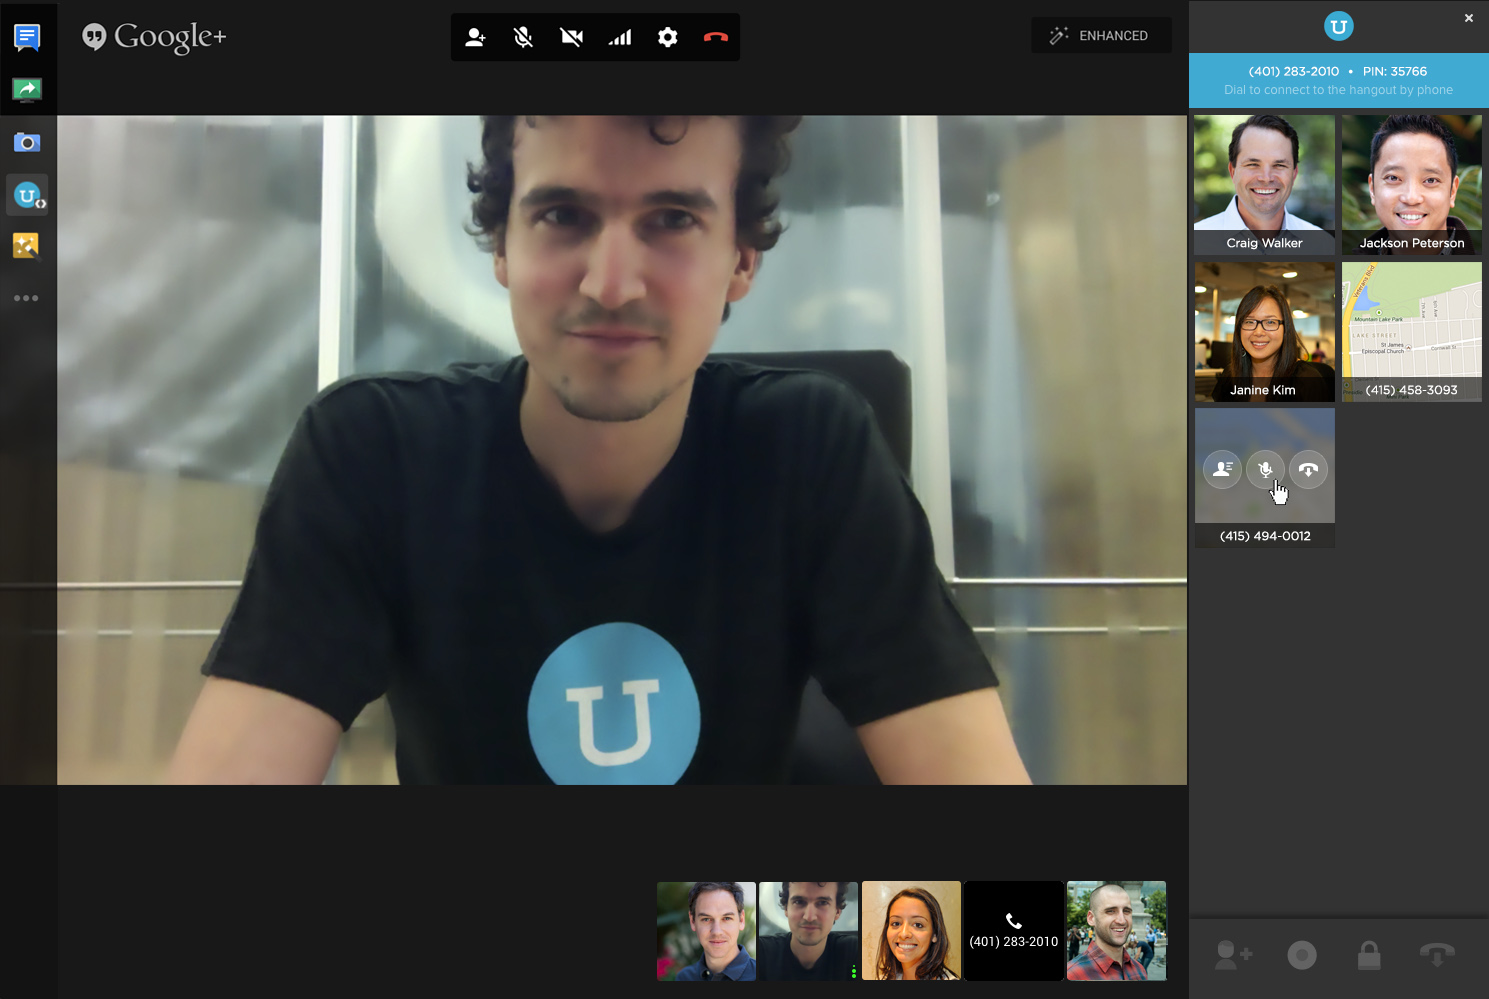
\includegraphics[width=0.58\textwidth,natwidth=610,natheight=642]{figs/uberconference_hangout.jpg}
  	\caption{UberConference integrate with Hangouts Screen shot\cite{tnw:uberconference}}
  	\label{fig:uberconference}
\end{wrapfigure}

\par The prototype system in this thesis ideally is to provide same rich media communication platform as the service provided by UberConference. In February of 2014, UberConference release the new feature which allow user to call into a Google Hangouts session with their mobile phone. The feature is shown in Figure \ref{fig:uberconference}, Once you have installed the UberConference app in Hangouts, people can join your call via phone with the help of a dedicated number. The prototype system will provide the same real-time communication service, but it allows the user to create a video conference based on \gls{webrtc} on browser by their mobile phone number and communicate with audio only mobile phone user as well. 

It will be more easier for user since they just need to remember their user credential related to their mobile phone number in order to use the prototype application rather than register another service user binding with private telephone number. And also it is more like usual telephone using because user call contacts based on their telephone number on the contact list. During the real-time conversation, the prototype application will provide user cooperation tools like instance message and file sharing in this development phase.

\subsection{Cube Slam}

\noindent Moreover, there is another important \gls{api}, \textit{RTCDataChannel} , can be used more creatively by developers to build web applications. The experiment usage cases, 'Cube Slam' and 'Webtorrent', are in this category which uses \textit{RTCDataChannel} to build \gls{p2p} data sharing without data going though the server to dispatch to other peers. It works more efficiently to handle the synchronization problem.

\par Cube Slam (shown in Figure \ref{fig:cube_slam}) is a Chrome Experiment built with \gls{webrtc} , play an old-school arcade game with your friends without downloading and installing any plug-ins. Cube Slam uses \textit{getUserMedia} to access user's webcam and microphone ,\textit{RTCPeerConnection} to stream user video to another user, and \textit{RTCDataChannel} to transfer the bits that keep the gameplay in sync. If two users are behind firewalls, \textit{RTCPeerConnection} uses a TURN  relay server (hosted on Google Compute Engine) to make the connection. However, when there are no firewalls in the way, the entire game happens directly peer-to-peer, reducing latency for players and server costs for developers.\cite{chrome:cube_slam}

\begin{figure}
	\centering
    	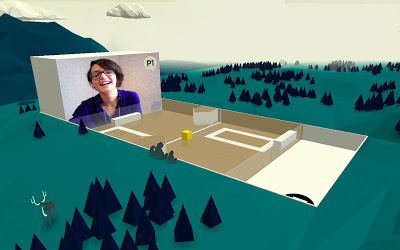
\includegraphics[width=0.8\textwidth,natwidth=610,natheight=642]{figs/cube_slam.jpg}
  	\caption{Cube Slam Game Over Screen}
  	\label{fig:cube_slam}
\end{figure}

\par The idea behind the Cube Slam is that using \textit{RTCDataChannel} to sync the player data in real-time to reduce the latency by peer to peer. \textit{RTCDataChannel} sends data securely, and supports an "unreliable" mode for cases where you want high performance but don't care about every single packet making it across the network. In the cases like games where low delay often matters more than perfect delivery, this ensures that a single stray packet doesn't slow down the whole app. The prototype application in this thesis will use WebSocket for data sharing instead of \textit{RTCDataChannel} because the media server using in this system is not support \textit{RTCDataChannel} yet, so it is not possible to create peer to peer session regarding to this issue. The \textit{RTCDataChannel} solution in prototype application will be discussed in Chapter \ref{chp:future_work}.

\subsection{Webtorrent}

\par The goal of project Webtorrent is to build a browser BitTorrent client that requires no install, no plugin, no extension, and fully-interoperates with the regular BitTorrent network. It uses \gls{webrtc} Data Channels for peer-to-peer transport. Since WebTorrent is web-first, it's simple for users who do not understand .torrent files, magnet links, NATs, etc. By making BitTorrent easier, it will be accessible to new swathes of users who were previously intimidated, confused, or unwilling to install a program on their machine to participate.\cite{github:webtorrent}

\par Since \gls{webrtc} is usually used for peer to peer communication, the \textit{RTCDataChannel} can be used in more creative way like Webtorrent. Although it need to keep the browser up and running on both ends and there will be no asynchronous nature into it, it does reduce the bandwidth required and it adds privacy as to who has access to the file being shared. Since the application can reach direct between browsers, it can use the data channel to create a low latency network, where data is shared directly without going through servers on the way. It is lower cost for the developer and more secure for the clients. For example, doing the same using a drastically larger number of web browser nodes as \gls{tor}\footnote{Tor (previously an acronym for The Onion Router) is free software for enabling online anonymity and censorship resistance. \gls{tor} directs Internet traffic through a free, worldwide, volunteer network consisting of more than five thousand relays to conceal a user's location or usage from anyone conducting network surveillance or traffic analysis.\cite{wiki:tor}}, increases the chance of privacy.This can reduce the need for “real” web servers to run services, and use those only as points of access into the dynamic network that is created ad-hoc.

\par This \textit{RTCDataChannel} usage is reasonable solution to the prototype system as well. However, the main focus of the prototype system is to integrate the \gls{webrtc} multimedia type with the \gls{voip} network against with traditional telephony network. It will not implement \textit{RTCDataChannel} function in the system, but this topic will be discussed in chapter \ref{chp:future_work}.

\section{SIP}
\noindent The prototype application in this thesis will be integrated with \gls{pstn} through \gls{sip} server. Therefore the application server implemented in this system will use \gls{sip} as signaling to communicate with \gls{sip} server to handle the signaling configuration with mobile/fixed phone end-point.

\subsection{What is SIP ?}
\noindent The \gls{sip} is a signaling communication protocol, widely used for controlling multimedia communication sessions such as voice and video calls over \gls{ip} networks.

\par The protocol defines the messages that are sent between endpoints which govern establishment, termination and other essential elements of a call. \gls{sip} can be used for creating, modifying and terminating sessions consisting of one or several media streams. \gls{sip} can be used for two-party (unicast) or multiparty (multicast) sessions. Other \gls{sip} applications include video conferencing, streaming multimedia distribution, instant messaging, presence information, file transfer, fax over \gls{ip} and online games.\cite{wiki:sip}

\par \gls{sip} works in conjunction with several other application layer protocols that identify and carry the session media. Media identification and negotiation is achieved with the \gls{sdp}. It is different key filed format than the \gls{webrtc} \gls{sdp}. For the transmission of media streams (voice, video) \gls{sdp} typically employs the \gls{rtp} or \gls{srtp}. For secure transmissions of \gls{sip} messages, the protocol can be encrypted with \gls{tls}.

\subsection{SIP Network Elements}
\noindent In normal \gls{sip} network, \gls{sip} defines user-agents as well as several types of server network elements. Two \gls{sip} endpoints can communicate without any intervening \gls{sip} infrastructure. However, this approach is often impractical for a public service, which needs directory services to locate available nodes on the network. In the system implemented of this thesis, the application server will play the roles as 'User Agent', 'Registrar' and 'Gateway' elements in the \gls{sip} network.

\noindent \textbf{User Agent}\cite{wiki:sip}:
\par A \gls{sip} \gls{ua} is a logical network end-point used to create or receive \gls{sip} messages and thereby manage a \gls{sip} session. A \gls{sip} \gls{ua} can perform the role of a \gls{uac}, which sends \gls{sip} requests, and the \gls{uas}, which receives the requests and returns a \gls{sip} response. These roles of \gls{uac} and \gls{uas} only last for the duration of a \gls{sip} transaction.

\noindent \textbf{Registrar}\cite{wiki:sip}:
\par A registrar is a \gls{sip} endpoint that accepts REGISTER requests and places the information it receives in those requests into a location service for the domain it handles. The location service links one or more \gls{ip} addresses to the \gls{sip} \gls{uri} of the registering agent. The \gls{uri} uses the sip: scheme, although other protocol schemes are possible, such as tel:. More than one user agent can register at the same \gls{uri}, with the result that all registered user agents receive the calls to the \gls{uri}.

\noindent \textbf{Gateway}\cite{wiki:sip}:
\par Gateways can be used to interface a \gls{sip} network to other networks, such as the \gls{pstn}, which use different protocols or technologies. In the prototype application, the application server is the gateway to interface a \gls{webrtc} WebSocket network. The working process will be covered in Chapter \ref{chp:sys_imp}.

\subsection{SIP messages}
\noindent Since the application server in this system will be used as \gls{sip} \gls{ua} and \gls{sip} Gateway, it will send \gls{sip} message requests to \gls{sip} server and receive \gls{sip} message requests from the \gls{sip} server.

\par One of the wonderful things about \gls{sip} is that it is a text-based protocol modeled on the request/response model used in \gls{http}. This makes it easy to debug because the messages are easy to construct and easy to see.  Contrasted with H.323\footnote{H.323 is a recommendation from the ITU Telecommunication Standardization Sector (ITU-T) that defines the protocols to provide audio-visual communication sessions on any packet network. The H.323 standard addresses call signaling and control, multimedia transport and control, and bandwidth control for point-to-point and multi-point conferences.\cite{wiki:h323}}, SIP is an exceedingly simple protocol.  Nevertheless, it has enough powerful features to model the behavior of a very complex traditional telephone \gls{pbx}.\cite{networkworld:sip}

\par There are two different types of \gls{sip} messages: requests and responses. The first line of a request has a method, defining the nature of the request, and a Request-\gls{uri}, indicating where the request should be sent.The first line of a response has a response code.

\noindent For sip requests, regarding to RFC 3261\cite{rfc:3261}, the application server in the system will use following \gls{sip} messages:

\begin{itemize}[topsep=-1em,parsep=0em,itemsep=0em]
 \item \textbf{REGISTER:} Used by a \gls{ua} to indicate its current \gls{ip} address and the \gls{url}s for which it would like to receive calls.
 \item \textbf{INVITE:} Used to establish a media session between user agents.
 \item \textbf{ACK:} Confirms reliable message exchanges.
 \item \textbf{CANCEL:} Terminates a pending request.
 \item \textbf{BYE:} Terminates a session between two users in a conference.
\end{itemize}

\noindent The \gls{sip} response types defined in RFC 3261 will be listened by application server in the following response codes\cite{wiki:sip_response_codes}:

\begin{itemize}[topsep=-1em,parsep=0em,itemsep=0em]
 \item \textbf{100 Trying:} Extended search being performed may take a significant time so a forking proxy must send a 100 Trying response.
 \item \textbf{180 Ringing:} Destination user agent received INVITE, and is alerting user of call.
 \item \textbf{200 OK:} Indicates the request was successful.
 \item \textbf{400 Bad Request:} The request could not be understood due to malformed syntax.
 \item \textbf{401 Unauthorized:} The request requires user authentication. This response is issued by \gls{uas}s and registrars.
 \item \textbf{408 Request Timeout:} Couldn't find the user in time. The server could not produce a response within a suitable amount of time, for example, if it could not determine the location of the user in time. The client MAY repeat the request without modifications at any later time.
 \item \textbf{480 Temporarily Unavailable:} Callee currently unavailable.
 \item \textbf{486 Busy Here:} Callee is busy.
\end{itemize}

\par By listening these \gls{sip} response, the application will send requests to either \gls{webrtc} browser client or \gls{sip} client to play as the gateway role in the system. This gateway mechanism will be introduced in Chapter \ref{chp:sys_design}.

\section{Prototype System Working Flow}

\noindent To connect with the traditional telephony network, the \gls{voip} system bridges the \gls{pstn} and the \gls{ip} network. \gls{voip} systems employ session control and signaling protocols to control the signaling, set-up, and tear-down of calls. They transport audio streams over \gls{ip} networks using special media delivery protocols that encode voice, audio, video with audio codecs, and video codecs as Digital audio by streaming media. In the prototype system, \gls{sip} signaling is used because of its widely usage and current target \gls{pstn} has \gls{sip} server support.

\begin{figure}
	\centering
    	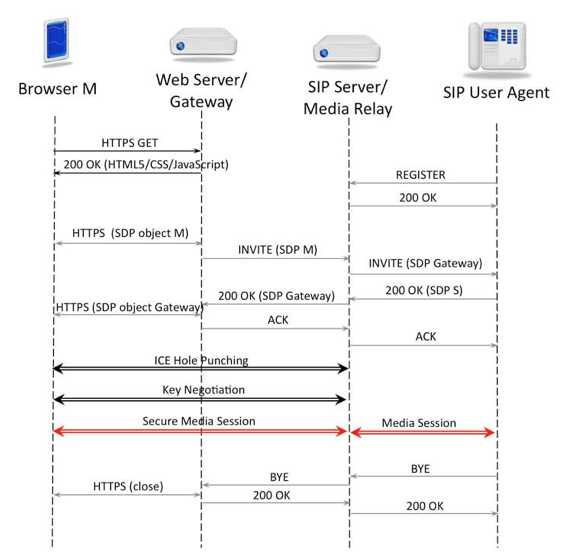
\includegraphics[width=0.60\textheight,natwidth=610,natheight=642]{figs/system_work_flow.png}
  	\caption{Prototype System Working Diagram \cite{inbook:sys_work_diagram}}
  	\label{fig:sys_work_diagram}
\end{figure}

\par The Figure \ref{fig:sys_work_diagram} shows the basic working flow of the prototype system. The Web Server/ Gateway is the application server in the prototyep system, it mainly bridges the \gls{webrtc} browser client with other \gls{webrtc} clients and the \gls{sip} network. The \gls{sip} server bridges the \gls{sip} network and \gls{pstn} network or traditional telephony network. And also the Media Relay server relay all the media stream from different end clients. In the prototype system, there is another media server besides the media relay function provided by \gls{sip} server because the media server needs to handle different media \gls{sdp} in signalings which are \gls{webrtc} \gls{sdp} and \gls{sip} \gls{sdp}. The media server used in the prototype system is provided by Dialogic, the Network Fuel company, which is called PowerMedia XMS v2.1\footnote{PowerMedia XMS is pre-integrated with a variety of application servers and signaling gateways with HTTP-to-SIP (H2S) functionality and rapidly integrates with others using its web API or standard interfaces.}. PowerMedia XMS acts as a WebRTC Media Gateway to mediate WebRTC media-plane differences from those of typical existing VoIP networks including encryption interworking, transcoding, and client-based NAT traversal support. The reason to use this media server is to avoid hard-code transition between \gls{webrtc} \gls{sdp} and \gls{sip} \gls{sdp}. Then the end client no matter is a \gls{webrtc} client or a \gls{sip} client, they will communicate with the same signaling client in their aspect.

\par Moreover, since the media server is used in this case, during the multiple end-point conversation, each end-point will only exchange their media stream to the single end-point on the media server (PowerMedia XMS server), it will make light client and centralized media server control. The benefit of this system architecture will be discussed more in the Chapter \ref{chp:sys_design}.

\par Therefore, in the Figure \ref{fig:sys_work_diagram}, all the end point keep using their own original signaling protocol to communicate with different servers of the prototype system in order to reach different scope end point.

\section{Prototype Working Scenario}

\noindent The prototype system in this thesis will pay more attention on the real-time communication usage of \gls{webrtc}. The main purpose of the system is to combine internet browser user and traditional telephony user without complicate instillation, plugin and extension. There are two typical working scenarios of the prototype system will be described below.

\subsection{Advanced 'one-number' communication platform}

\par Adam is a typical Facebook\footnote{Facebook is an online social networking service.} user and he does synchronize his contact list through Google Contacts\footnote{Google Contacts is Google's contact management tool that is available in its free email service Gmail, as a standalone service, and as a part of Google's business-oriented suite of web apps Google Apps.\cite{wiki:google_contacts}} by his smart phone. Now his operator provides user credential from his telephone number to him. Then Adam just login on his operator 'FellowPhone' web page, now he can import his contacts list through his Google contact list. After that, he can see if his contact person is online by using the same web application 'FellowPhone' or not. He can also import his Facebook friends list and fulfill the friends list with his contacts list information. Therefore, Adam can see if his facebook friends online or not. If his facebook friends/ Google contacts are online and use 'FellowPhone' web application from their operator, Adam can invite them have a video conference otherwise his friends are not online then he can still invite them into the video conference but through his friends mobile phone with only audio sound.

\par During the video conference, Adam can send his online friends files and instance messages (website links, video links and so on). Moreover, his offline friends in the same conference will get the same information as text \gls{sms}. Adam can reach his friends wherever they are and no matter if they are online or not as long as they have their mobile phone. 

\subsection{Multiple doctors consultation room}

\par Eve is a 70-year-old lady, she lives with her children in their house. But at the day time, her children go to work, she need take care of herself. She has appointment with her doctor about her backache. But she can not go to hospital or family doctor office by her own. Then she uses her mobile phone to call her family doctor. Her family doctor, Isak, uses the prototype service from his company and operator. When Eve call to her doctor for help, Isak answered her phone and tried to get her previous medical information from his working system. Then he found out that Eve had other doctor about her back treatment before. He can just login in the prototype system and find out if the other doctor is at work (online in the system). Eve's previous doctor, Stella, she has the treatment log about Eve. She got invitation to join the current conversion with Isak and Eve. She can send message to Isak and share the treatment log with Isak if it is necessary. She can also listen to the talk between Isak and Eve about the new update of the treatment to give suggestion. Isak can ask for more different doctors in the system for advice and consultation to help for Eve case.

\par In Eve aspect, she only calls doctor Isak, but she can got help from more than one doctor at the same time. If it is necessary, she can use the computer to login the same system to have video conference with different doctors for her case. The only thing required for her is a telephone number and a mobile phone.
\chapter{Prototype System Design}
\label{chp:sys_design}

\noindent In this chapter, it will cover system design progress of the prototype system along with explanation and analysis. The prototype system is designed based on preliminary studies from previous chapter. There will be different implementation solutions to the prototype working scenario  discussed and evaluated in this chapter. After evaluating these solutions, it will come up with the fit solution to the prototype working scenario. 

\section{Prototype System Network}

\noindent In the original \gls{webrtc} application implementation, it uses mesh network because \gls{webrtc} means to be the peer to peer communication method bypass the third party server. However, the prototype system will use centralized server network to control and route the communication channels between different types end points. In this section, it will describe the reason to use centralized server network rather than mesh network.

\subsection{Mesh Network}

\par A mesh network is a network topology in which each node (called a mesh node) relays data for the network, the illustration of the network is shown in Figure \ref{fig:mesh_network}. All nodes cooperate in the distribution of data in the network. When \gls{webrtc} designed, it considered as mesh network using and take the advantages of the mesh network. Mesh network provides point-to-point line configuration makes identification and isolation of faults easy. The messages travel through a dedicated line in the mesh network, directly to the intended recipient. More privacy and security are thus enhanced. If a fault occurs in a given link of the network, only those communications between that specific pair of devices sharing the link will be affected.\cite{wiki:mesh_network}

\par However, with the design of mesh network, the more extensive the network, in terms of scope or of physical area, the greater the investment necessary to build it will be, due, among other considerations, to the amount of cabling and the number of hardware ports it will require.
Every device must be connected to every other device, installation and re-connection are difficult. The huge bulk of the wiring can often be greater than the available space in the ceiling or under floors can accommodate.

\begin{figure}
	\centering
    	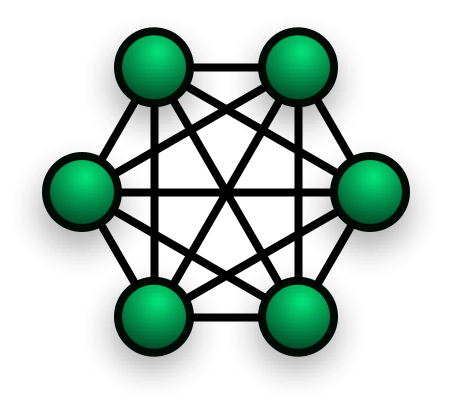
\includegraphics[width=0.40\textwidth,natwidth=610,natheight=642]{figs/mesh_network.png}
  	\caption{Illustration of a Mesh Network \cite{wiki:mesh_network}}
  	\label{fig:mesh_network}
\end{figure}

\par Considering the prototype system case, a real-time communication system, the scaling problem in the feature will eventually be the top priority issue. With the mesh network, it is difficult and impossible to scale the system with the control since the network scales by the unknown end points.There is a similar production application called \textit{appear.in}. It is a video conversations application with up to 8 people in the browser. \textit{appear.in} uses peer-to-peer communication, meaning that the video streams are sent directly between the browser clients. Nothing is stored on the server and all the communication is encrypted over SSL. But the limit of 8 clients in one conversation is mainly because the client browser it self can not handle too many peer connections. Because according to mesh network, every client in the conversation would set up one unique \gls{webrtc} \textit{RTCPeerConnection} object and one unique media stream exchange channel on the client, it consumes client computer resources a lot. Thus, the prototype system will not use mesh network as the system network architecture in order to avoid the future scaling problem. The advantages of the mesh network is well implemented in the \gls{webrtc} api, then the prototype system will keep these advantages to keep the point-to-point lines isolated with each other and keep the point-to-point communication more private and secure.

\subsection{Centralized Network}

\par Centralized network is a type of network where all users connect to a central server, which is the acting agent for all communications. This server would store both the communications and the user account information. Most public instant messaging platforms use a centralized network. It is also called as centralized server-structure.\cite{webopedia:centralized_network} It is similar network architecture shown in Figure \ref{fig:system_network}.

\begin{figure}
	\centering
    	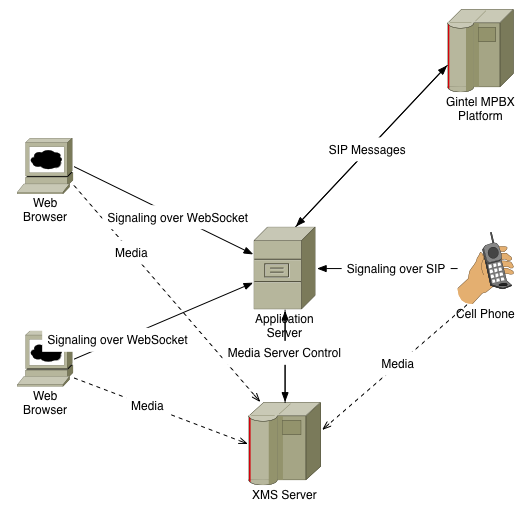
\includegraphics[width=0.70\textwidth,natwidth=610,natheight=642]{figs/system_network.png}
  	\caption{Prototype System Network}
  	\label{fig:system_network}
\end{figure}

\par The advantages of centralized server network are centralized control of the system, centralized observation of the system and light requirement for the client . In the prototype system, there are application server and media server to handle the application logic business and media stream exchange business(see in Figure \ref{fig:system_network}). Although every clients communicate with application to do the \gls{webrtc} signaling, the media stream is not go through the application server, it goes through the media server only. Furthermore, every client creates single \gls{webrtc} connection pair with the one resource on XMS media server, the advantage of point-to-point line configuration is still kept in the system. As client aspect, it still makes peer-to-peer media stream connection based on \gls{ssl}. The function of XMS media server is to combine more than two of the peer resources into one conference resource in order to set up the multimedia conference channel. More detail about XMS media server handling will be covered in Chapter \ref{chp:sys_imp}.

\par The other important advantage of centralized server network is that the application server and media server can observe the condition and quality of the real-time conversation to administrate the routing and quality improvement process. For this reason, the media stream quality on every end point will be more stable and better quality control. Since the prototype application is to integrate with traditional telephony network, it is important to provide similar quality control and fault tolerant mechanism in the prototype system.

\par Regarding to centralized server network, it is possible to use different signaling protocol on \gls{webrtc} browser clients to application server and \gls{sip} clients to application server. The benefits to have different signaling protocols in prototype system is to keep the \gls{webrtc} clients and the \gls{sip} clients in their own traditional working process, there will be no compatibility for both sides. The application server in the prototype system will play the role as a gateway to decide which signaling protocol needs to be used to communicate with different end clients. Moreover, it will be easier for different existing \gls{webrtc} commercial services and \gls{sip} commercial services to integrate with the prototype system in order to communicate with each other network.

\par The disadvantage of centralized server network would be the application server and media server itself as well. During the development of the prototype system, it is easy to figure out that the machine to host the application server and media server is not powerful enough to handle too much client connection and media stream connection. When it meets the scaling issue, the application server and media server need to be distributed in multiple server host and consume powerful server machines. The cost of the entire system is higher than the mesh network solution.

\par As a conclusion of these two types network architecture, for this prototype system, it will be centralized server network, Figure \ref{fig:system_network}, to be implemented because it is more suit to the goal of this thesis to be integrated with traditional telephony network usage.

\section{Prototype Implementation Framework}

\noindent Since \gls{webrtc} is a web \gls{api}, the prototype application will be a web application. There are many different web application framework nowadays to provide rich-client web application. In this section, some of the web application framework will be discussed to figure out which framework is best solution to the prototype scenario. Furthermore, application server will be discussed with different implementation solutions since it does signaling and bridge the \gls{sip} network and clients.

\subsection{Client Implementation Framework}

\noindent To choose web application framework to implement the client application in this thesis scenario, the main fact is that if the web  application framework is fit to the real time communication application and if the framework has the ability to integrate with \gls{webrtc} \gls{api}. After research about these kinds of web application framework, it narrows down to three main framework to discuss.

\textbf{AngularDart :}

\par AngularDart is a framework for building web-apps in Dart. Dart is an open-source Web programming language developed by Google. It is a class-based, single inheritance, object-oriented language with C-style syntax. It supports interfaces, abstract classes, reified generics, and optional typing. Static type annotations do not affect the runtime semantics of the code. Instead, the type annotations can provide documentation for tools like static checkers and dynamic run time checks.\cite{wiki:dart} Because most of the script language is not type strict, it is easy to mess up the code and value type in script language. Moreover, Dart has Dart-to-JavaScript compiler,dart2js, it makes Dart can be used in client and server both. Addition to AngularJs framework in Dart, it provide a professional web application structure to the developer to implement. More about AngularJs notable features will be covered in the later AngularJs solutions. 

\par The \gls{webrtc} implementation in Dart is in this repository: \url{https://github.com/br1anchen/AngularDart_webRTC}. The Code Snippet \ref{code:dart_webrtcctrl} shows the main controller in AngularDart. The line 5 is to import \gls{webrtc} client class \textit{speack\_client.dart}, the class has all the \gls{webrtc} \gls{api}s implemented in Dart. Line 23 is to initialize the \textit{SpeakerClient} object and set the arguments WebSocket url and room name. They are used for signaling in WebSocket Protocol.

\par However, after implementation of client application and server back-end in Dart. There is a critical bug in the current Dartium browser. The Dart SDK ships with a version of the Chromium web browser modified to include a Dart \gls{vm}. Dartium browser can run Dart code directly without compilation to JavaScript. It is intended as a development tool for Dart applications, rather than as a general purpose web browser. When embedding Dart code into web apps, the current recommended procedure is to load a bootstrap JavaScript file, "dart.js", which will detect the presence or absence of the Dart \gls{vm} and load the corresponding Dart or compiled JavaScript code, respectively, therefore guaranteeing browser compatibility with or without the custom Dart VM.\cite{wiki:dart} 
\par The issue noticed as \textbf{RtcPeerConnection.addIceCandidate results in a NotSupportedError: Internal Dartium Exception} in the Dart Google Project issues.\cite{bug:dartium} The sample code in the \gls{webrtc} Dart implementation shown in Code Snippet \ref{code:dart_add_ice}, line 1 is to create \textit{RTCPeerConnection} object. From line 5 to line 13 is to send message to server when \textit{RTCPeerConnection} object get \textit{onIceCandidate} event witch \gls{ice} candidate information. Line 17 is to bind the message listener event to Dart function \textit{onCandidate.listen}. From line 21 to line 30 is the Dart function to create \textit{RTCIceCandidate} object and add to \textit{RTCPeerConnection} object. The bug issue happens on line 27, when the \textit{RTCPeerConnection} call \textit{addIceCandidate} function, it is not allowed to have callback function in current version Dartium.

\begin{lstlisting}[caption={Add IceCandidate in Dart},label={code:dart_add_ice}]
var pc = new RtcPeerConnection(_iceServers, _dataConfig);

....

    pc.onIceCandidate.listen((e){
      if (e.candidate != null) {
        _send('candidate', {
          'label': e.candidate.sdpMLineIndex,
          'id': id,
          'candidate': e.candidate.candidate
        });
      }
    });
    
...

get onCandidate => _messages.where((m) => m['type'] == 'candidate');

...

onCandidate.listen((message) {
	var candidate = new RtcIceCandidate({
		'sdpMLineIndex': message['label'],
        'candidate': message['candidate']
    });

    _connections[message['id']].addIceCandidate(candidate,(){},(e){
    		print('add ice candidate error');
    });
});

...
\end{lstlisting}

\par There is a work around solution in one Stack Overflow\footnote{Stack Overflow is a privately held website, the flagship site of the Stack Exchange Network, created in 2008 by Jeff Atwood and Joel Spolsky, as a more open alternative to earlier Q\&A sites such as Experts Exchange.} answer: \url{http://stackoverflow.com/questions/20404312/how-to-call-addicecandidate-in-dart}. The fix method is to use \textit{js-interop} library to use pure JavaScript code in Dart to call the \gls{webrtc} Web \gls{api} instead of Dart \gls{webrtc} interface.
\par Mozilla's Brendan Eich, who developed the JavaScript language, stated that:

\textit{"I guarantee you that Apple and Microsoft (and Opera and Mozilla, but the first two are enough) will never embed the Dart VM. So 'Works best in Chrome' and even 'Works only in Chrome' are new norms promulgated intentionally by Google. We see more of this fragmentation every day. As a user of Chrome and Firefox (and Safari), I find it painful to experience, never mind the political bad taste."}\cite{wiki:dart}

\par Since Dart in not support to most modern web browser like FireFox, will not be used in this prototype.

\textbf{Sipml5 + webrtc2sip:}

\begin{figure}
	\centering
    	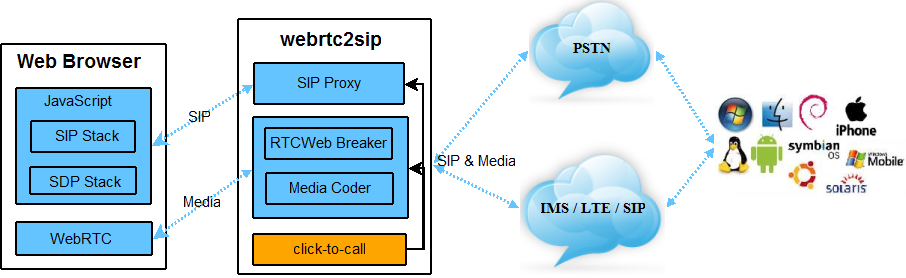
\includegraphics[width=0.80\textwidth,natwidth=610,natheight=642]{figs/sipml5_network.png}
  	\caption{Sipml5 and webrtc2sip Network}
  	\label{fig:sipml5_network}
\end{figure}

\par Sipml5 is the world's first open source \gls{html5} \gls{sip} client entirely written in JavaScript for integration in social networks (FaceBook, Twitter, Google+), online games, e-commerce websites, email signatures. The media stack rely on \gls{webrtc}. The client can be used to connect to any \gls{sip} or \gls{ims} network from your preferred browser to make and receive audio/video calls and instant messages.\cite{website:sipml5}

\par Sipml5 provides whole client solution to communicate with other kind of signaling real-time communication network. The \gls{sip} and \gls{sdp} stacks are entirely written in JavaScript and the network transport uses WebSockets as per draft-ibc-sipcore-sip-websocket. However the community of sipml5 is not so active, the issues and source code on sipml5 source code project website \url{https://code.google.com/p/sipml5/} are not updated regularly. Like the Figure \ref{fig:sipml5_network} showing, it works with media gateway webrtc2sip.

\par webrtc2sip is a smart and powerful gateway using \gls{webrtc} and \gls{sip} to turn your browser into a phone with audio, video and \gls{sms} capabilities. The gateway allows your web browser to make and receive calls from/to any \gls{sip}-legacy network or \gls{pstn}.
The gateway contains four modules: \gls{sip} Proxy, RTCWeb Breaker, Media Coder, Click-to-Call.\cite{website:webrtc2sip}

\par In the prototype working scenario, it is necessary to have media gateway to communicate with \gls{sip}-legacy network. Since the current \gls{pstn} using in this prototype go through Gintel \gls{mpbx} Platform, it is necessary to use RTCWeb Breaker to be able to connect the browser to a SIP-legacy endpoint.

\par Therefore, the test for Sipml5 and webrtc2sip solution is based on the live demo \url{http://sipml5.org/call.htm}. But even with the RTCWeb Breaker, the test is still failed to call any number through the target \gls{pstn}. Since most of the source code of these two framework are hidden from the encapsulation, it is impossible to debug which part of the testing system is the problem. In the test, the registration for \gls{sip} client is successful, but there are 'too long message' in the \gls{sip} error message got from the \gls{sip} server. It means that the sipml5 and webrtc2sip network architecture is not compatible with the target \gls{pstn} through the Gintel \gls{mpbx} Platform. This solution can not be used in the prototype system.

\textbf{AngularJs + Socket.IO:}

\par AngularJS is built around the belief that declarative programming should be used for building user interfaces and wiring software components, while imperative programming is excellent for expressing business logic. The framework adapts and extends traditional \gls{html} to better serve dynamic content through two-way data-binding that allows for the automatic synchronization of models and views. As a result, AngularJS de-emphasizes \gls{dom} manipulation and improves testability. Angular follows the \gls{mvc} pattern of software engineering and encourages loose coupling between presentation, data, and logic components. Using dependency injection, Angular brings traditional server-side services, such as view-dependent controllers, to client-side web applications. Consequently, much of the burden on the backend is reduced, leading to much lighter web applications.\cite{wiki:angularjs}

\par AngularJs is perfect for single-page web application, the framework features provide developer a professional way to structure the web application in JavaScript. Moreover, the developer community of AngularJs is quite active, there are a lot of different Angular module services to provide the different interfaces against different web \gls{api}s.In the prototype, there will be several third party Angular module library to be used in order to integrate with some advanced JavaScript library or web \gls{api}s in Angular style.

\par Socket.IO is a JavaScript library for realtime web applications. It has two parts: a client-side library that runs in the browser, and a server-side library for node.js. Both components have a nearly identical \gls{api}. Socket.IO primarily uses the WebSocket protocol, but if needed can fallback on multiple other methods, such as Adobe Flash sockets, \gls{jsonp} polling, and \gls{ajax} long polling, while providing the same interface. Although it can be used as simply a wrapper for WebSocket, it provides many more features, including broadcasting to multiple sockets, storing data associated with each client, and asynchronous I/O.\cite{wiki:socketio} In the prototype application, Socket.IO is used in WebSocket protocol because the WebSocket protocol provides full-duplex communications channels over a single \gls{tcp} connection. Then the communication channel will be active and real time between the clients and server during the whole connecting procedure. It fits the real time communication application requirement.

\par After test demo client application implemented in AngularJs and Socket.IO frameworks, it works fine with the basic \gls{webrtc} functions and simple \gls{sip} registration against \gls{sip} server to target \gls{pstn}. The final decision of the client implementation framework of prototype system will be AngularJs and Socket.IO.

\subsection{Server Implementation Framework}

\noindent Since the client side will use Socket.IO as communication protocol library, the server back-end in the prototype system will use Node.js as server implementation framework. In thist section, more detail about comparison and differences of Node.js against traditional web service back-end (in Java, ASP .NET\footnote{ASP.NET is a server-side Web application framework designed for Web development to produce dynamic Web pages. It was developed by Microsoft to allow programmers to build dynamic web sites, web applications and web services.\cite{wiki:asp}} or \gls{php}) will be covered.

\textbf{Node.js:}

\par Node.js is a software platform for scalable server-side and networking applications. Node.js applications are written in JavaScript, and can be run within the Node.js runtime on Mac OS X, Windows and Linux with no changes. Node.js applications are designed to maximize throughput and efficiency, using non-blocking I/O(Input/Output) and asynchronous events. Node.js applications run single-threaded, although Node.js uses multiple threads for file and network events. Node.js is commonly used for real time applications due to its asynchronous nature.\cite{wiki:nodejs}

\par At high levels of concurrency server needs to go to asynchronous non-blocking, otherwise there will be blocking \gls{io} on the server to delay other \gls{io} process. The issue is that if any part of the server code blocks, on the traditional server framework,  it is going to need a thread. And at these levels of concurrency, it can’t keep creating threads for every connection. Then the whole codepath needs to be non-blocking and synchronized, not just the \gls{io} layer. This is where Node excels, shown in Figure \ref{fig:nodejs}. The main difference between Figure \ref{fig:nodejs} and Figure \ref{fig:threading_java} is the way of server to handle the requests. On Node.js server, it handles all the requests in asynchronous threads after the requests are delegated from event loop. But on multiple threaded server, programming language used on these server mostly does not support for the async pattern. Then it would not matter whether raw \gls{nio} performance is better than Node or any other benchmark result.

\begin{figure}
	\centering
    	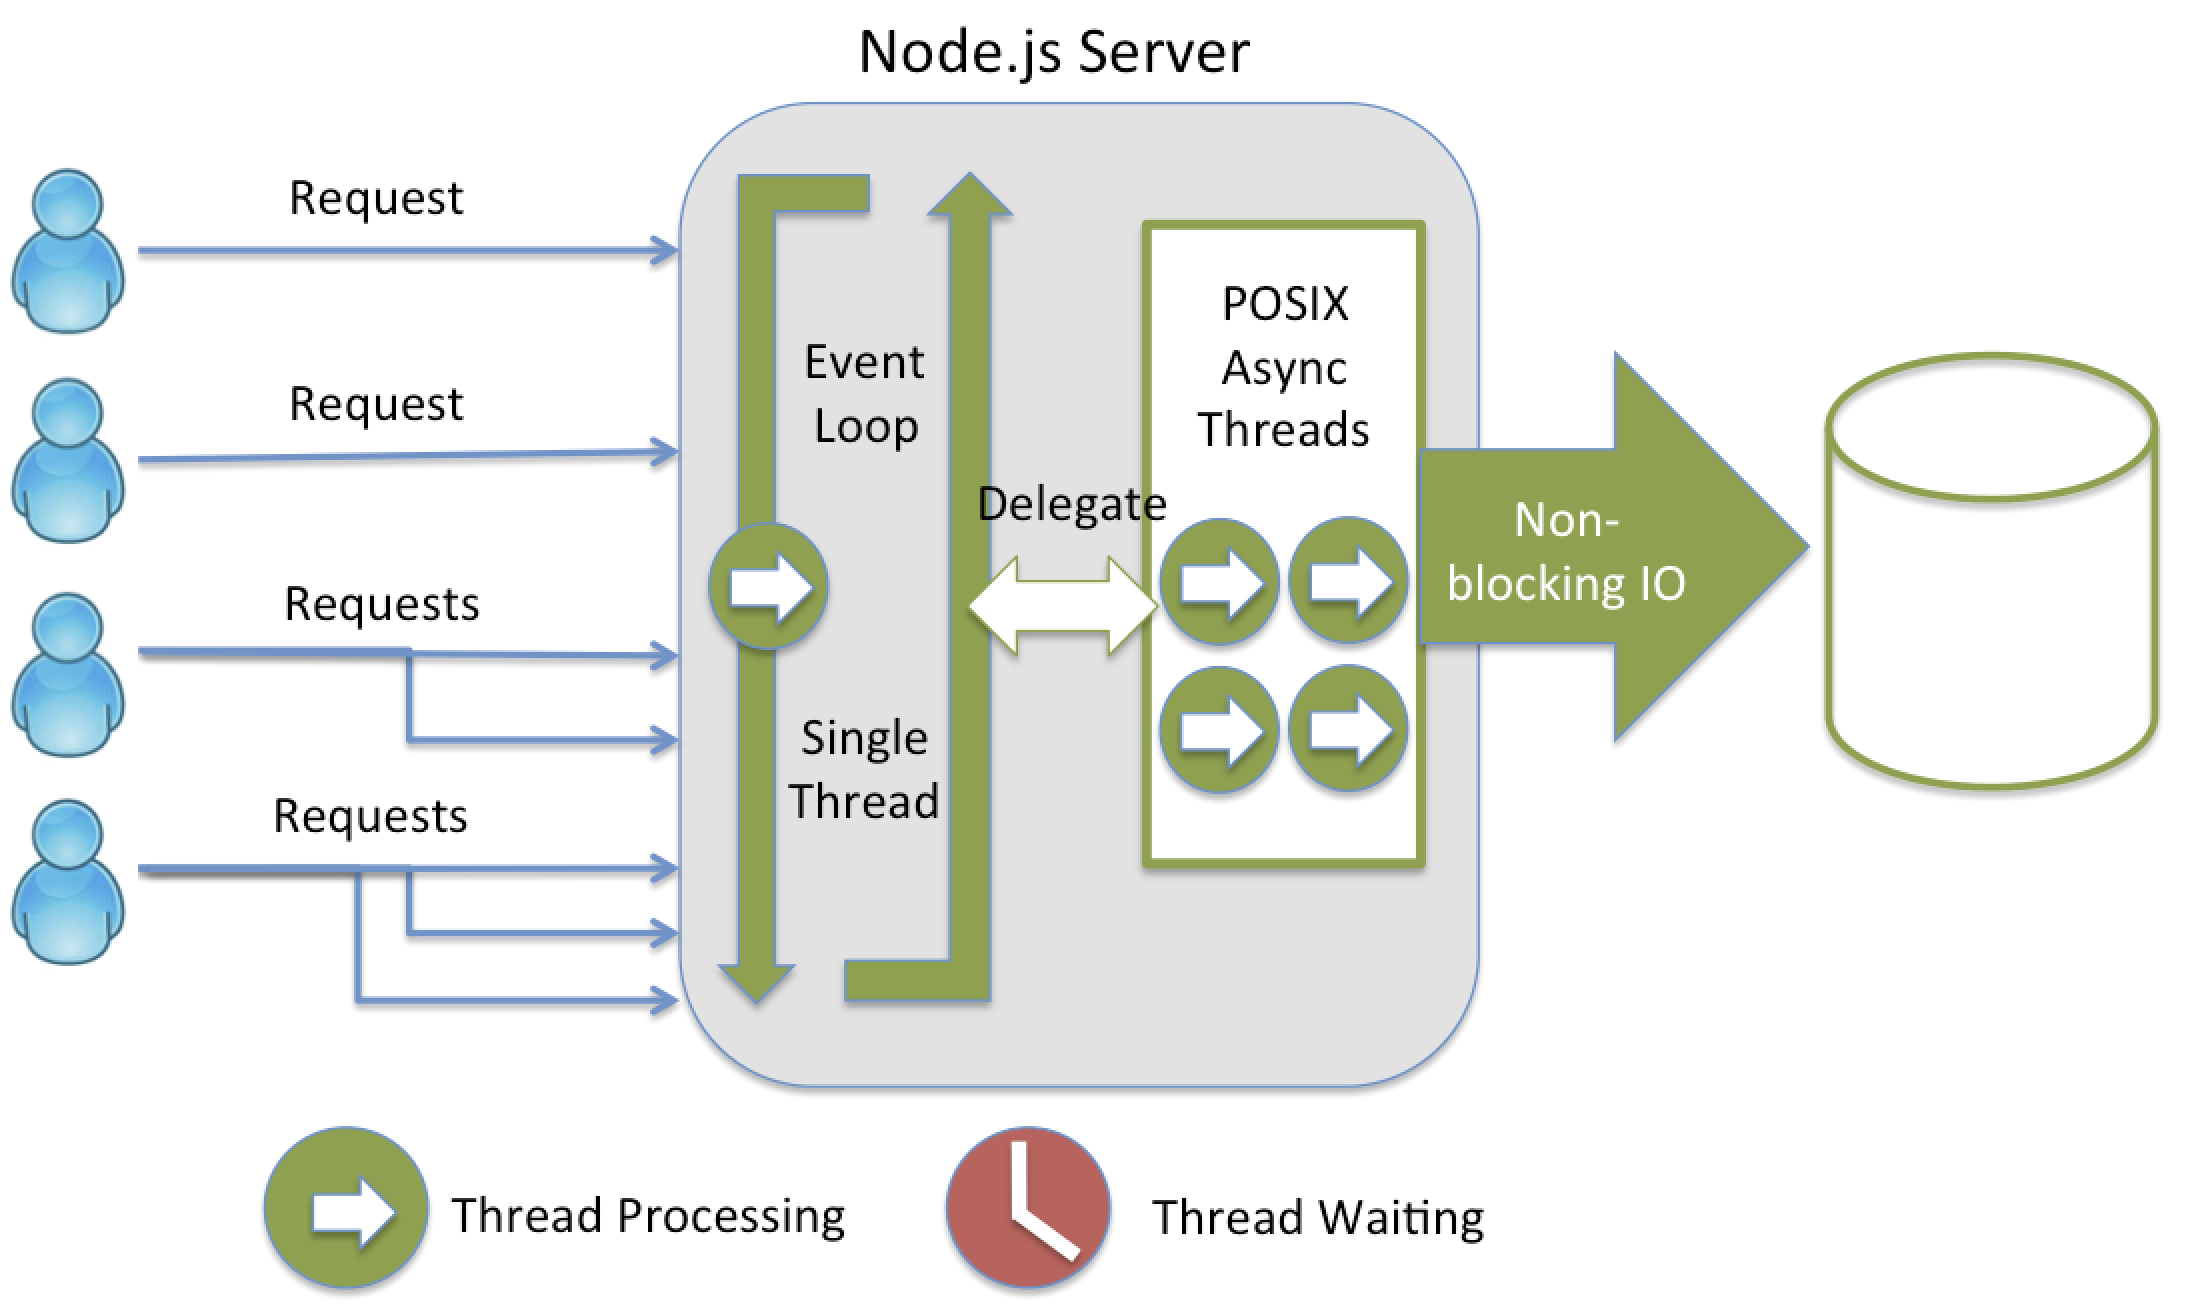
\includegraphics[width=0.60\textwidth,natwidth=610,natheight=642]{figs/nodejs.png}
  	\caption{Node.js Non-blocking I/O\cite{strongloop:nodejs}}
  	\label{fig:nodejs}
\end{figure}

\begin{figure}
	\centering
    	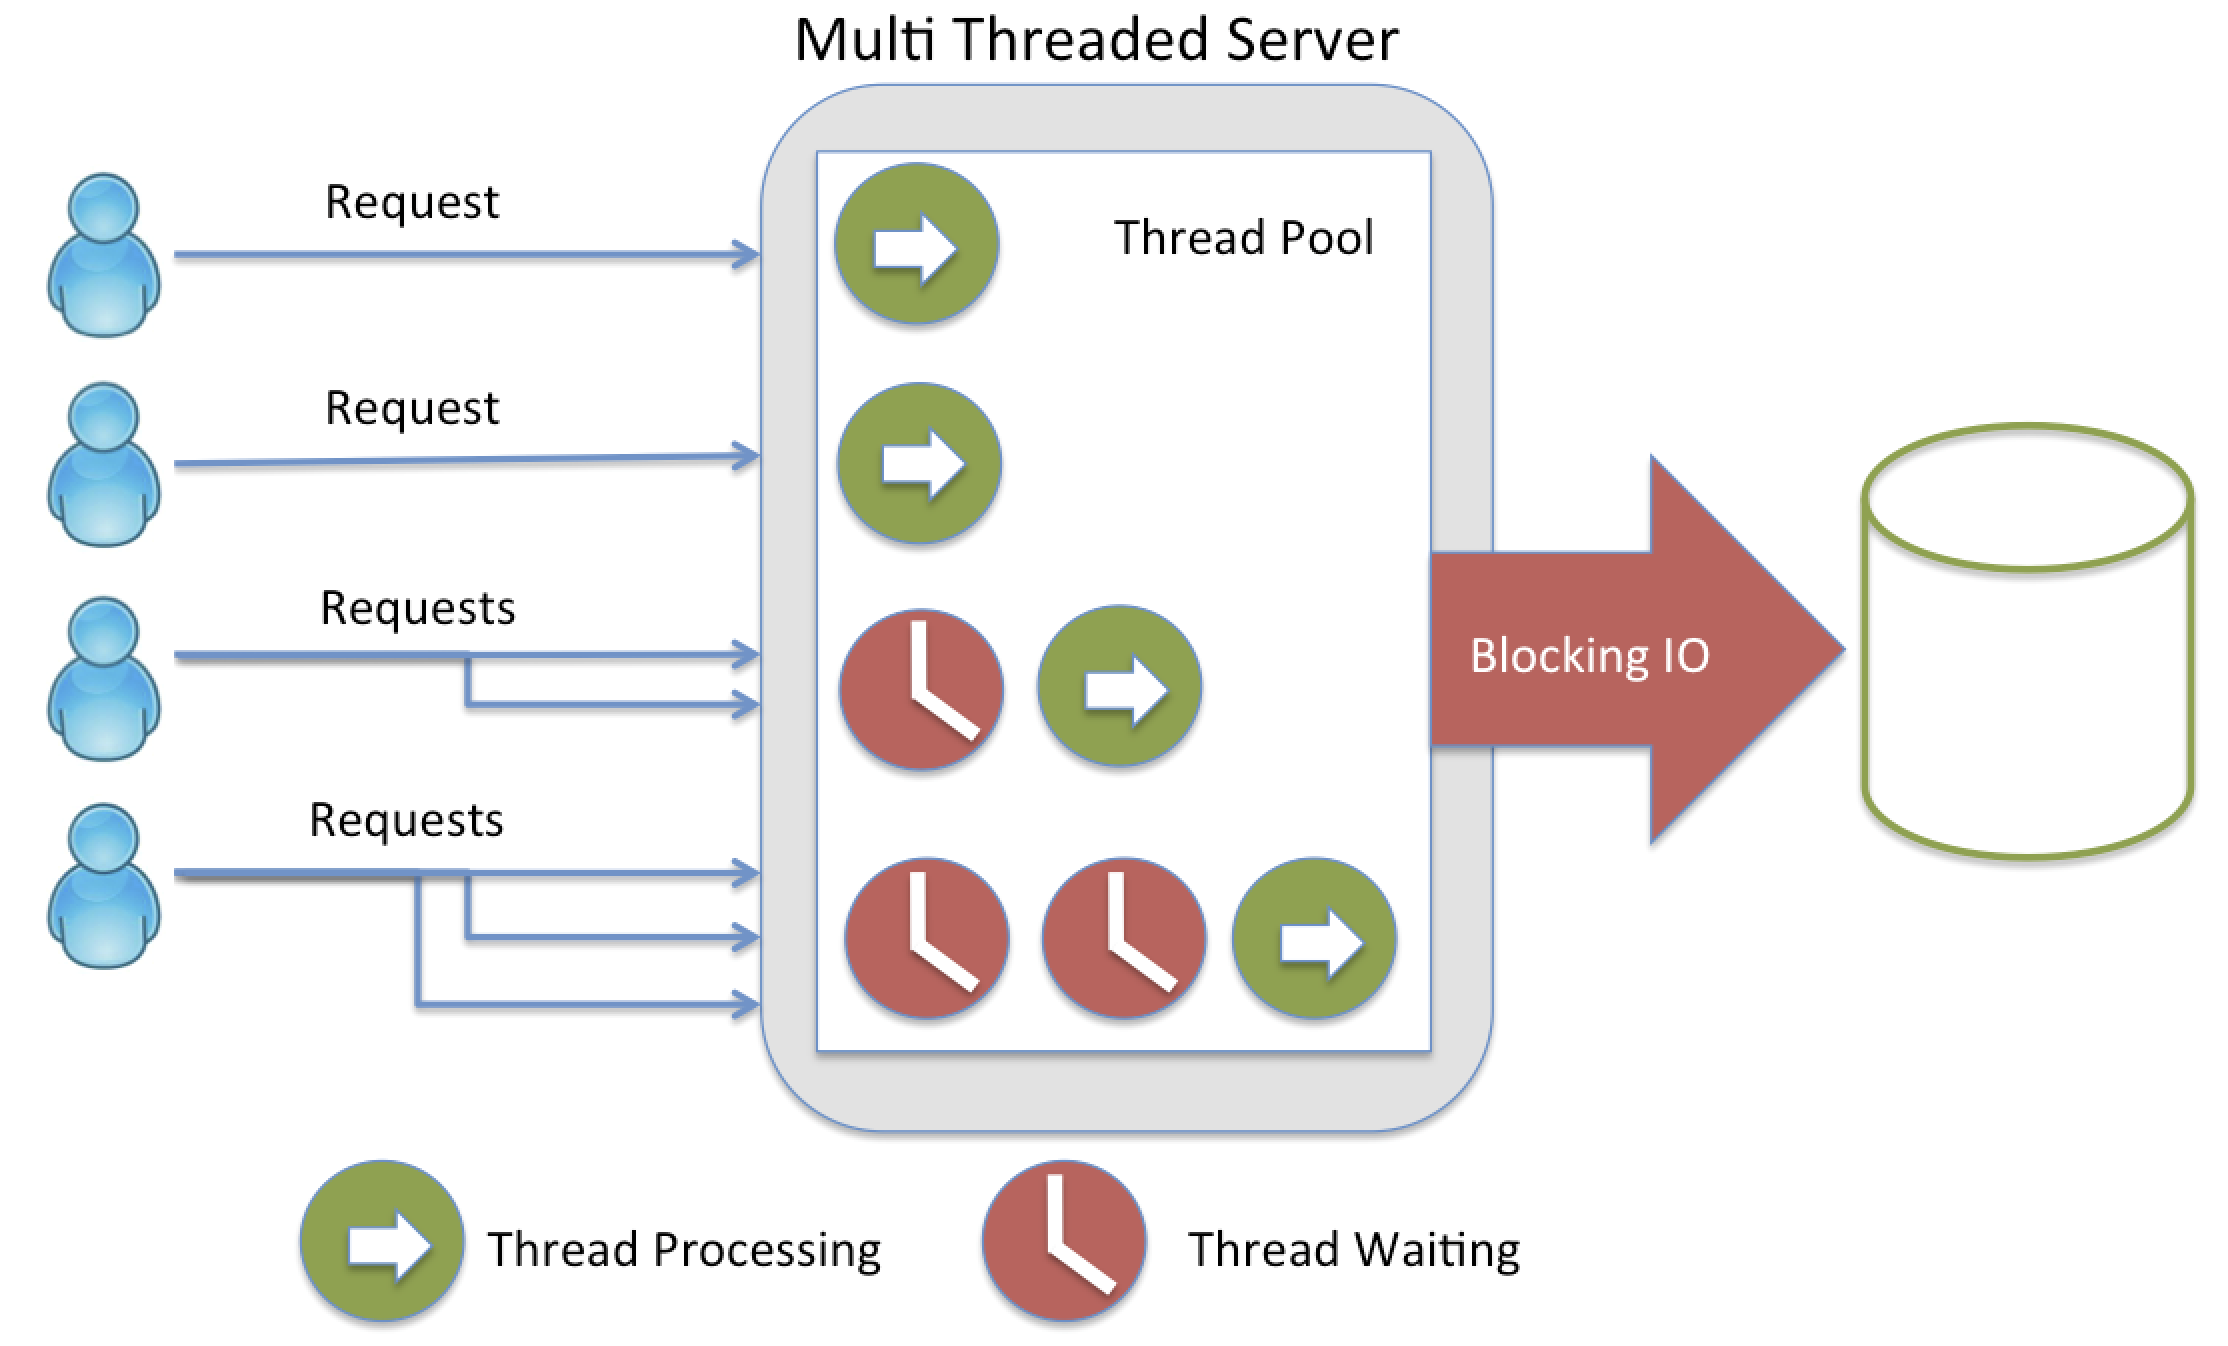
\includegraphics[width=0.60\textwidth,natwidth=610,natheight=642]{figs/threading_java.png}
  	\caption{Multiple Threaded Server\cite{strongloop:nodejs}}
  	\label{fig:threading_java}
\end{figure}

\par Since the prototype is a real-time communication application, it is better to use Node.js as back-end server rather than multiple threaded server. Moreover, the WebSocket protocol framework used on client side has good server side solution based on Node.js, it makes the development of the prototype system much easier to implement. The prototype system is a centralized server network, the communication between application server to XMS server will be hold on normal \gls{http}/\gls{https} protocol, Node.js provides these protocol communication as well, no need to host any additional web server software such as Apache\footnote{The Apache HTTP Server, commonly referred to as Apache, is a web server application notable for playing a key role in the initial growth of the World Wide Web.\cite{wiki:apache}}.

\par For the other part of the prototype, \gls{sip} network, there is a existing Node.js module can be used as \gls{sip} stack on Node.js server. sip.js is a \gls{sip} stack for node.js. It implements tranaction and transport layers as described in RFC3261\footnote{SIP: Session Initiation Protocol}.\cite{github:sipjs} Although sip.js is not production framework yet, it is one of the few \gls{sip} stack library in Node.js. It provides \gls{sip} message parser, \gls{udp}/\gls{tcp}/ \gls{tls} based transport
transactions and digest authentication. These features are quite fit to the prototype requirement and quite handy to implement.

\par There will be more detail about \gls{sip} implementation on sip.js library on Node.js in the later chapter. Since it is not mature library, there are quite few stuff need to be fixed through the development.

\textbf{Mobicents Sip Servlets}

\begin{figure}
	\centering
    	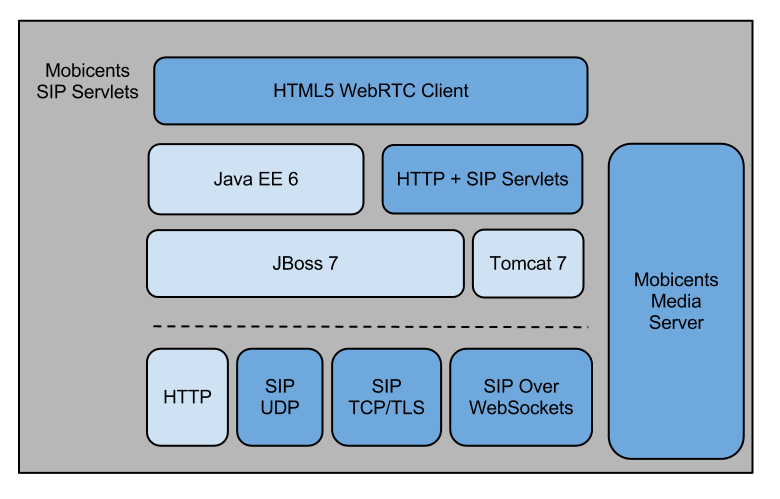
\includegraphics[width=0.60\textwidth,natwidth=610,natheight=642]{figs/mobicents.png}
  	\caption{Mobicents SIP Servlets\cite{code:mobicents}}
  	\label{fig:mobicents}
\end{figure}

\par Mobicents \gls{sip} Servlets delivers a consistent, open platform on which to develop and deploy portable and distributable \gls{sip} and Converged \gls{jee} services.  It is the first open source certified implementation of the \gls{sip} Servlet v1.1 (\gls{jsr} 289 Spec) on top of Tomcat\footnote{Apache Tomcat (or simply Tomcat, formerly also Jakarta Tomcat) is an open source web server and servlet container developed by the Apache Software Foundation (ASF).\cite{wiki:tomcat}} and JBoss\footnote{WildFly, formerly known as JBoss AS, or simply JBoss, is an application server authored by JBoss, now developed by Red Hat. WildFly is written in Java, and implements the Java Platform, Enterprise Edition (Java EE) specification. It runs on multiple platforms.\cite{wiki:jboss}} containers and strive to feature best performances, security, foster innovation and develop interoperability standards between \gls{sip} Servlets and \gls{jslee} so that applications may exploit the strengths of both. The \gls{jain}\footnote{Java APIs for Integrated Networks (JAIN) is an activity within the Java Community Process, developing APIs for the creation of telephony (voice and data) services.\cite{wiki:jain}}-\gls{sip} Reference implementation is leveraged as the \gls{sip} stack and Mobicents \gls{jain} \gls{slee}\footnote{An accelerated development and deployment environment of new IP Multimedia Subsystem (IMS) services for convergent fixed- mobile network environments.\cite{website:slee}} is used as the \gls{slee} implementation.

\par The architecture of the Mobicents \gls{sip} Servlets is shown in Figure \ref{fig:mobicents}. As it described, Mobicents \gls{sip} Servlets provide multiple transport protocol include \gls{http}, \gls{udp}, \gls{tcp} and WebSocket. These transport protocols are fit the prototype requirements, but on the application layer, it has two application server need to be host, one is JBoss and the other is Tomcat 7, JBoss is support for all the \gls{sip} stack transport and Tomcat 7 is support for \gls{http} requests. JBoss is the gateway to communicate with \gls{sip} network and Tomcat host the application server to communicate with media server to handle the real-time multimedia stream.

\par It is quite nice system architecture to work with, but it need powerful server machine to host two web application server on it. Considering Node.js solution, it is not easy to maintain the system since developer need to configure on two different web application server to handle different protocol transportation and client and server are implemented in different programming languages.

\par After implemented one test application by Mobicents \gls{sip} Servlets framework, it is hard for developer to program the lower level source codes, for example \gls{sip} message headers field modification and WebSocket transport template. The test application successes to set up conversation session between \gls{webrtc} browser client and \gls{sip} client. But when the media stream exchange on XMS server(media server), there is only one way audio(from browser to phone) in the conversation. Because the \gls{sip} transport layer is encapsulated in the Mobicents \gls{sip} Servlets framework, it is hard to modify it to do more test if the bug is in the transport layer of the framework. The source code of this test application is owned by Gintel AS.

\par As a conclusion, the prototype system will use Node.js as server side back-end to communicate with AngularJs client application on Socket.IO protocol.
\chapter{Prototype System Implementation}
\label{chp:sys_imp}

\noindent In this chapter, it will cover implementation progress of the prototype system along with explanation and analysis. The prototype system is implemented based on solution research from chapter \ref{chp:sys_design}.

\section{Prototype Functions}

\noindent Based on the study from previous chapter, there are some real time features are implemented in the prototype system, they are shown in the Table \ref{tab:functions}. The final version of prototype application is shown in Figure \ref{fig:webgui_call_outgoing}, it is the main page of the web application client. The green notification message on the left shows that there is an outgoing call from the client to the 'Brian Chen' contact.

\begin{figure}
	\centering
    	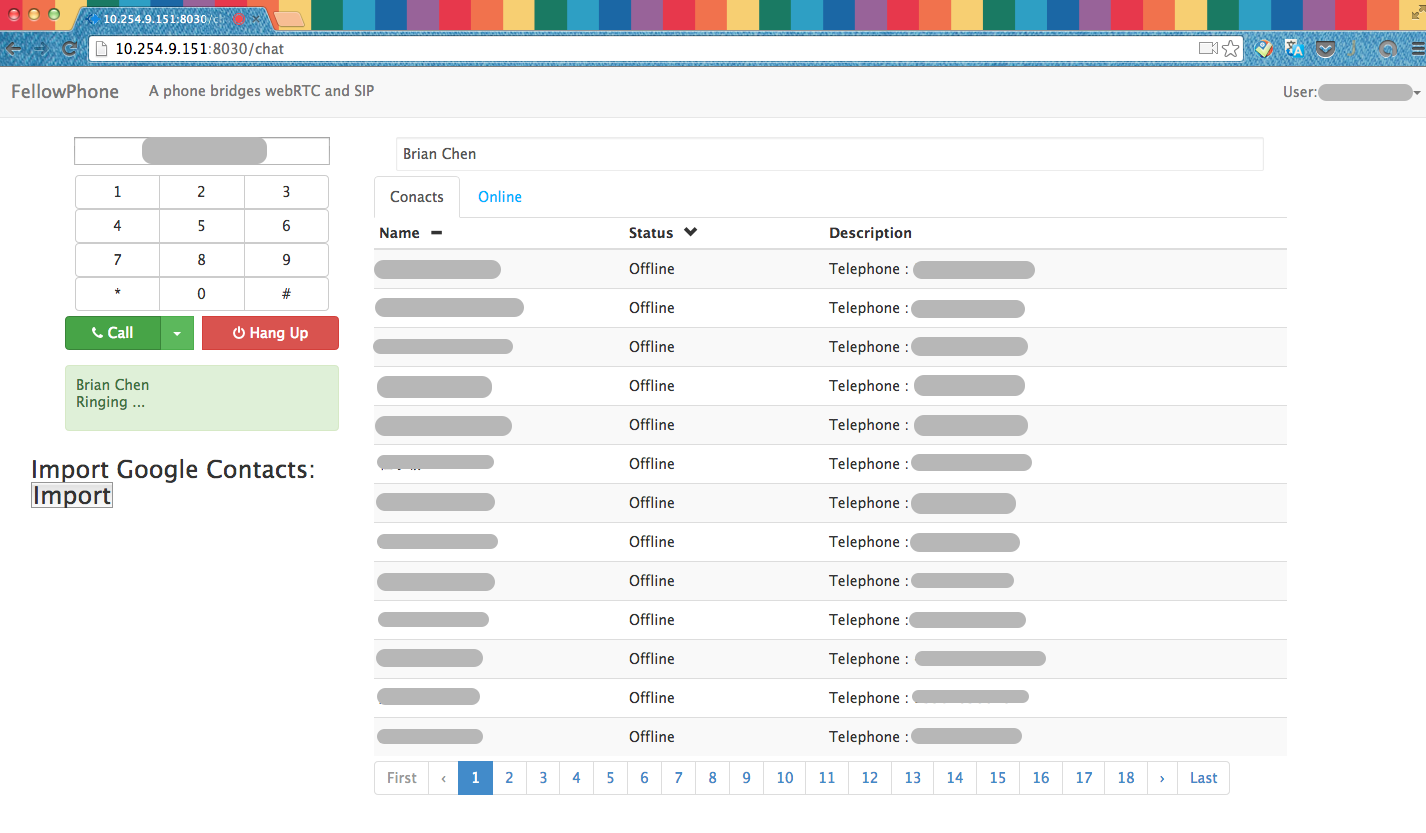
\includegraphics[width=0.90\textwidth,natwidth=610,natheight=642]{figs/webgui_call_outgoing.png}
  	\caption{Prototype Application Calling Outbound Mobile Number}
  	\label{fig:webgui_call_outgoing}
\end{figure}

\begin{table}
\caption{\label{tab:functions}: Prototype System Functions}
\centering
\begin{tabular}{| c | p{3cm} | p{5.5cm} |}
\hline
No & Function & Detail \\ \hline
\#1 & Single Call & Web browser client application can call outbound \gls{sip} client and receive outbound \gls{sip} client calling \\ \hline
\#2 & Multiple Users Video Conference & Multiple Web browser clients can have video conference \\ \hline
\#3 & Multiple Clients Conference & Multiple web browser client and single \gls{sip} client conference session \\ \hline
\#4 & Forward Call & When one of two web browser clients leaves the current three end points(2 \gls{webrtc} clients and 1 \gls{sip} client) conference, this \gls{sip} phone call will be forwarded to the only \gls{webrtc} client in the current conference session \\ \hline
\#5 & Instance Message & Instance Message chatting board in the current conference session \\ \hline
\#6 & Instance Message to \gls{sms} & \gls{sms} messages will be sent to \gls{sip} client phone which is in the current video conference session \\ \hline
\#7 & Files Sharing & Files can be shared in the current video conference session with the \gls{webrtc} client in the conference \\ \hline
\#8 & Google Contacts Import & User can import their Google Contacts to the application clients for synchronize contacts list \\ \hline
\#9 & Web Notification & All the necessary application notification will be display through the browser web notification message \\
\hline
\end{tabular} 
\end{table}

\par In the prototype system function Table \ref{tab:functions}, functions \#1 to \#4 is the basic telephony functions, they are implemented by \gls{webrtc} \gls{api}, application server and XMS media server. The detail about them will be covered in \gls{webrtc} \gls{api}s Implementation section, \gls{sip} Implementation section and XMS Media Server section since they are the real time communication function for \gls{webrtc} and \gls{sip} clients.

\par Function \#5 is implemented by Socket.IO framework which is discussed in previous chapter. The implementation detail will be covered in Socket.IO Implementation section.
Function \#6 is the advanced function along with the function \#5, it is implemented in \gls{msg} which will be discussed in \gls{sms} Messaging section in the later chapter.

\par Function \#7 is implemented by Delivery.js framework not the original \gls{webrtc} \textit{RTCDataChannel}, more detail will be discussed in Files Sharing section.

\par Function \#8 is another advanced feature provided by prototype application, it is implemented by Google Contacts \gls{api} which will be covered in AngularJs Framework Implementation section as the sample code section for AngularJs framework.

\par Function \#9 is to make the web application more user friendly and more like traditional telephone usage scenario. It will not be covered in this thesis since the user experience is not the top priority object for this thesis.

\section{WebRTC APIs Implementation}

\noindent \gls{webrtc} components are accessed with JavaScript \gls{api}s. Currently in development are the Network Stream \gls{api}, which represents an audio or video data stream, and the PeerConnection \gls{api}, which allows two or more users to communicate browser-to-browser. Also under development is a DataChannel \gls{api} which enables communication of other types of data for real-time gaming, text chat, file transfer, and so forth. Because the media server used in prototype system is not support for DataChannel yet, the DataChannel \gls{api} will not be covered in this section. \textit{RTCDataChannel} \gls{api} will be discussed in chapter \ref{chp:future_work}.

\begin{figure}
	\centering
    	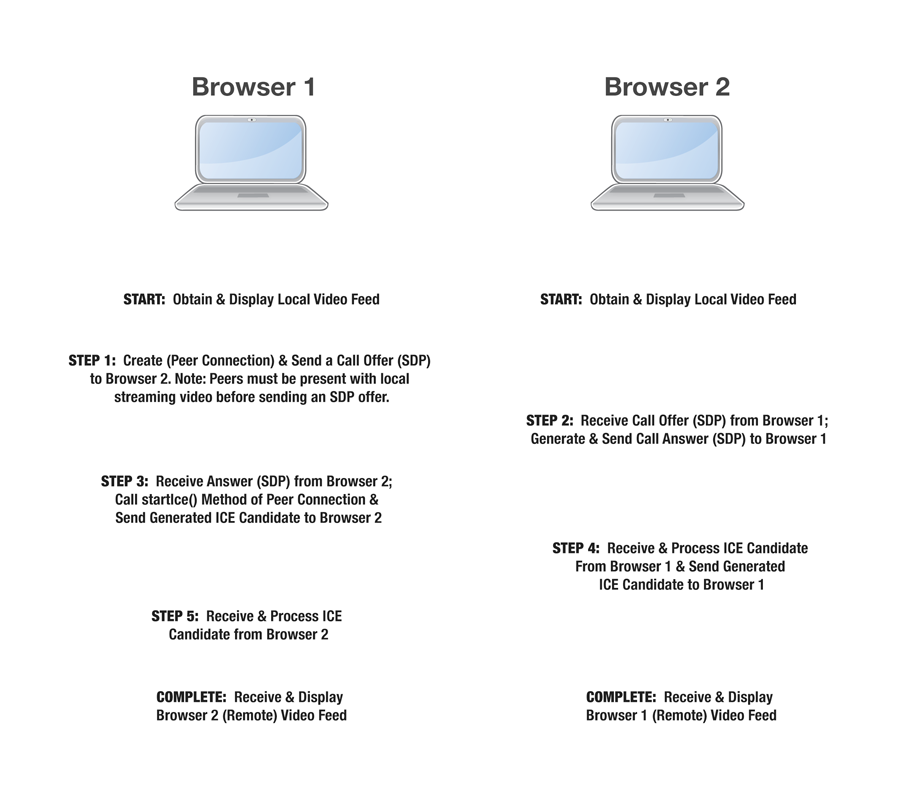
\includegraphics[height=0.50\textheight,natwidth=610,natheight=642]{figs/webrtc_diagram.png}
  	\caption{WebRTC two peer communication process\cite{mdn:p2pwebrtc}}
  	\label{fig:webrtc_diagram}
\end{figure}

\subsection{MediaStream API}

\par The MediaStream \gls{api} represents synchronized streams of media. For example, a stream taken from camera and microphone input has synchronized video and audio tracks. In order to obtain local media, the start step for both peers in Figure \ref{fig:webrtc_diagram}, the \gls{webrtc} \gls{api} provides \textit{navigator.getUserMedia()} function to get the video and audio stream from user. For privacy reasons, a web application’s request for access to a user’s microphone or camera will only be granted after the browser has obtained permission from the user. Each MediaStream has an input, which might be a MediaStream generated by \textit{navigator.getUserMedia()}, and an output, which might be passed to a video element or an \textit{RTCPeerConnection}.
\par The \textit{getUserMedia()} method takes three parameters:

\begin{itemize}[topsep=-1em,parsep=0em,itemsep=0em]
 \item A constraints object.
 \item A success callback which, if called, is passed a MediaStream.
 \item A failure callback which, if called, is passed an error object.
\end{itemize}

\par The Code Snippet \ref{code:get_user_media} shows that how the prototype application implements \textit{getUserMedia()} function, it is encapsulated in \textit{WebRTCService} (service is a reusable business logic independent of views in prototype application regarding to AngularJs framework\footnote{AngularJS is an open-source web application framework, maintained by Google and community, that assists with creating single-page applications, one-page web applications that only require HTML, CSS, and JavaScript on the client side.\cite{wiki:angularjs}}).For the constraints object in parameters, the prototype application set 'audio' and 'video' value to true because it is necessary for the real-time communication application to have video and audio stream both.

\begin{lstlisting}[caption={Get User Media Stream function},label={code:get_user_media}]
var media_constraints = {audio: true,video: true};

function _setMediaStream(){
	WebRTCService.getUserMedia(media_constraints,
  								_handleUserMedia,
  								_handleUserMediaError);
  	console.log('Getting user media with constraints', 
  				media_constraints);
}
\end{lstlisting}

\par \textit{getUserMedia()} function is currently available in Chrome, Opera and Firefox. Almost all of the \gls{webrtc} \gls{api}s are slightly different based on different browsers implementation. In the Code Snippet \ref{code:webrtc_service}, there are two blocks to make all the set up process for FireFox and to make the same set up process for Google Chrome. Because \gls{webrtc} is not standard Web \gls{api} yet, so the implementation on different browsers are different as well. For example, the \textit{RTCPeerConnection} \gls{api} in Firefox is \textit{mozRTCPeerConnection} but in Google Chrome it is \textit{webkitRTCPeerConnection}. In order to make the \gls{webrtc} application works on more browsers, the client side need to figure out which kind of browser is using on the machine then call the corresponding \gls{webrtc} \gls{api}s. Google provides a JavaScript shim called \textit{adapter.js}. It is maintained by Google, it abstracts away browser differences and spec changes. For Angularjs framework used by prototype application, then the \textit{WebRTCService} is implemented to be integrated with \textit{adapter.js} function to achieve the goal of compatibility.

\par However, the prototype application in this thesis will only focus on Google Chrome browser\footnote{Google Chrome is a freeware web browser developed by Google. It used the WebKit layout engine until version 27 and, with the exception of its iOS releases, from version 28 and beyond uses the WebKit fork Blink.\cite{wiki:google_chrome}} to simplify the development process because \gls{webrtc} lower level implementation on different browsers are different and hard to track the issues. Then most of the results in this thesis is based on the application performance of Google Chrome browser. The reason to choose Google Chrome browser rather than other browser because \gls{webrtc} is the technology rapidly pushed by Google and Google Chrome browser has the most market share in the world. As of March 2014, StatCounter estimates that Google Chrome has a 43\% worldwide usage share of web browsers, making it the most widely used web browser in the world.\cite{wiki:google_chrome} However, Google changes a lot to improve the performance of \gls{webrtc} on Google Chrome browser, then it makes the \gls{webrtc} \gls{api}s work differently on different version of Google Chrome browser. In the Code Snippet \ref{code:webrtc_service}, from line 19 to line line 29 is the sample case to distinguish the difference among different version of Google Chrome to handle the \textit{RTCPeerConnection} \gls{ice} server constraint implementation.

\begin{lstlisting}[caption={WebRTCService.js in application client},label={code:webrtc_service}]
angular.module('webrtcDemo.services').
	factory('WebRTCService',function () {
		
		...

		function _setRTCElement() {

			if(navigator.mozGetUserMedia){
				...
			}else if(navigator.webkitGetUserMedia){
				...

			  // Creates iceServer from the url for Chrome.
			  _createIceServer = function(url, username, password) {
			    ...
			    if (url_parts[0].indexOf('stun') === 0) {
			      ...
			    } else if (url_parts[0].indexOf('turn') === 0) {
			      if (_webrtcDetectedVersion < 28) {
			        // For pre-M28 chrome versions use old TURN format.
			        var url_turn_parts = url.split("turn:");
			        iceServer = { 'url': 'turn:' + username + '@' + url_turn_parts[1],
			                      'credential': password };
			      } else {
			        // For Chrome M28 & above use new TURN format.
			        iceServer = { 'url': url,
			                      'credential': password,
			                      'username': username };
			      }
			    }
			    return iceServer;
			  };

			  ...
			}else{
				console.log("Browser does not appear to be WebRTC-capable");
			}

		}

		return {
			...
		}
	});	
	
\end{lstlisting}

\par Since \gls{webrtc} \gls{api}s is not standard \gls{api} yet, the prototype application in this thesis will not pay too much work-load on compatibility for different browsers platform. More detail about this issue will be discussed in the Chapter \ref{chp:future_work}.

\subsection{RTCPeerConnection API}

\noindent The step 1 of Figure \ref{fig:webrtc_diagram} is that the caller peer set up a communication process, it simply creates \textit{RTCPeerConnection} then send a \gls{webrtc} offer(by calling \textit{createOffer()} function and sending WebSocket message with \gls{sdp}) with local \gls{sdp} to the other peer. In the prototype system, it will send \gls{webrtc} offer to the application server, then the application server will check if the receiver is a \gls{webrtc} client or \gls{sip} to send different type of offer message(It will be covered in later of this chapter).

\par To set up peer connection, the \textit{RTCPeerConnection} \gls{api} sets up a connection between two peers. In this context, “peers” means two communication endpoints on the World Wide Web. Instead of requiring communication through a server, the communication is direct between the two entities. In the specific case of \gls{webrtc}, a peer connection is a direct media connection between two web browsers. This is particularly relevant when a multi-way communication such as a conference call is set up among three or more browsers. Each pair of browsers will require a single peer connection to join them, allowing for audio and video media to flow directly between the two peers. 

\par To establish peer connection, it requires a new \textit{RTCPeerConnection} object. The only input to the \textit{RTCPeerConnection} constructor method is a configuration object containing the information that \gls{ice}, will use to “punch holes” through intervening \gls{nat} devices and firewalls. The Code Snippet \ref{code:create_peer_connection} shows the create \textit{RTCPeerConnection} object and set three listener (\textit{onicecandidate},\textit{onaddstream},\textit{onremovestream}) to trigger the handlers to deal with the \gls{ice} candidate event and remote stream add/remove events.

\par The \textit{RTCPeerConnection} \gls{api} has two arguments to set, one is configuration object for peer connection and the other is constraint object (set transparent protocol and encryption) for peer connection, these value are shown in Code Snippet \ref{code:create_peer_connection} line 1 to line 10. In the showing case, the prototype is using \gls{stun} servers for different browser aspect, and set the \gls{rtc} channel encryption protocol to \gls{dtls}\footnote{In information technology, the Datagram Transport Layer Security (DTLS) protocol provides communications privacy for datagram protocols. DTLS allows datagram-based applications to communicate in a way that is designed to prevent eavesdropping, tampering, or message forgery.\cite{wiki:dtls}} and enable the \gls{rtc} DataChannel.

\par Because in Firefox, \gls{webrtc} media transparent channel is only based on \gls{dtls} protocol, and in latest version Google Chrome, \gls{dtls} is supported, then in the prototype application, it will use \gls{dtls} protocol to exchange the media stream.

\par There are two \gls{api}s to handle the \textit{RTCIceCandidate} object which contains \gls{ice} information data. One is \textit{onicecandidate} listener to trigger the function to handle the new \textit{RTCIceCandidate} data object. The other one is \textit{addIceCandidate} function, which is shown in the Code Snippet \ref{code:add_remote_ice}, to add the new \textit{RTCIceCandidate} data object to the remote/local peer connection session description field. As Code Snippet \ref{code:add_remote_ice} shown, the \textit{RTCIceCandidate} object has three attributes, \textit{sdpMLineIndex} is the media line index in the \gls{sdp}, \textit{sdpMid} is the media id which differ it is video or audio in the \gls{sdp} and \textit{candidate} is the \gls{ip} address and other detail of this media source.

\begin{lstlisting}[caption={Create Peer Connection function},label={code:create_peer_connection}]
pc_config = WebRTCService.webrtcDetectedBrowser() === 'firefox' ?
  			{'iceServers':[{'urls':'stun:stun.services.mozilla.com'}]} :
  			{'iceServers':[{'urls': 'stun:stun.l.google.com:19302'}]};

pc_constraints = {
			  'optional': [
			    {'DtlsSrtpKeyAgreement': true},
			    {'RtpDataChannels': true}
			  ]
			};
			
function _createPeerConnection(){

	try {
		pc = WebRTCService.peerConnection(pc_config, pc_constraints);
		pc.onicecandidate = _handleIceCandidate;
		console.log('Created RTCPeerConnnection with:\n' +
		      '  config: \'' + JSON.stringify(pc_config) + '\';\n' +
		      '  constraints: \'' + JSON.stringify(pc_constraints) + '\'.');
	} catch (e) {
		console.log('Failed to create PeerConnection, exception: ' + e.message);
		alert('Cannot create RTCPeerConnection object.');
		return;
	}
	pc.onaddstream = _handleRemoteStreamAdded;
	pc.onremovestream = _handleRemoteStreamRemoved;

}
\end{lstlisting}

\begin{lstlisting}[caption={Add Remote IceCandidate function},label={code:add_remote_ice}]
var candidate = WebRTCService.RTCIceCandidate({
					    	sdpMLineIndex:data.content.label,
					    	sdpMid:data.content.id,
					    candidate:data.content.candidate
				});
pc.addIceCandidate(candidate);

\end{lstlisting}

\par There are difference between Firefox and Google Chrome to handle the \textit{RTCIceCandidate} content in the \gls{sdp} while sending the offer to the other peer. In Firefox, it waits for all the \textit{RTCIceCandidate} data is fetched from \gls{stun}/\gls{turn} server then send it with \gls{webrtc} offer message. However, in Google Chrome, it sends the \gls{webrtc} offer message first, then update the local \gls{sdp} with new coming \textit{RTCIceCandidate} data one by one. Then in the prototype system, it needs to handle these differences by listening the \textit{endIceCandidate} event on application. After client fetches all the \textit{RTCIceCandidate} data, it sends an \textit{endIceCandidate} message to the application server to send the complete \gls{webrtc} offer message to the other peer.

\par In the step 2 of Figure \ref{fig:webrtc_diagram}, after the caller \textit{RTCPeerConnection} run \textit{createOffer()} function to send offer to callee through signaling channel, the callee need run \textit{createAnswer()} function to ask the \gls{stun}/\gls{turn} server to find the path for each other peer and create the answer with \gls{sdp} content. \gls{sdp} is intended for describing multimedia communication sessions for the purposes of session announcement, session invitation, and parameter negotiation. \gls{sdp} does not deliver media itself but is used for negotiation between end points of media type, format, and all associated properties.\cite{wiki:sdp} Before \textit{RTCPeerConnection} use \textit{createOffer()} function to send a \gls{webrtc} offer to the callee, it is required to be present with local streaming video, like Figure \ref{fig:webrtc_diagram} mentioned.

\par \gls{webrtc} clients need to ascertain and exchange local and remote audio and video media information, such as resolution and codec capabilities. Signaling to exchange media configuration information proceeds by exchanging an offer and an answer using the \gls{sdp}. The \textit{createOffer()} function and \textit{createAnswer()} function both have callback function to handle the \gls{sdp} either to call \textit{setLocalDescription()} by caller or call \textit{setRemoteDescription()} by callee when callee gets the caller's \gls{sdp} from \gls{webrtc} offer. The Code Snippet\ref{log:webrtc_answer_sdp} shown is the \gls{webrtc} answer \gls{sdp} from the callee when the callee end-point decide to accept this conversion session.

\par The sample \gls{sdp} from the prototype application is shown in Code Snippet \ref{log:webrtc_answer_sdp}. Line 2 in Code Snippet \ref{log:webrtc_answer_sdp} is the field 'o', it describes originator, session identifier, username, id, version number and network address. It usually means that where this package comes from. Line 7 and line 17 are field 'm', it describes media name and transport address. And line 11,12 and line 27,28 are the relevant lines for audio and video media field, they describes media filed 'candidate' attributes, in the sample case of Code Snippet \ref{log:webrtc_answer_sdp}, they are the \gls{ice} candidate from the \gls{stun}/\gls{turn} server. These are important fields regarding to the prototype system because they are used in XMS server and application server of the prototype system to exchange the media stream.

\begin{lstlisting}[caption={Sample \gls{webrtc} Answer \gls{sdp}},label={log:webrtc_answer_sdp}]
sdp: v=0
o=xmserver 1399363527 1399363528 IN IP4 10.254.9.135
s=xmserver
c=IN IP4 10.254.9.135
t=0 0
a=ice-lite
m=audio 49152 RTP/SAVPF 0 126
a=rtpmap:0 PCMU/8000
a=sendrecv
a=rtcp:49153
a=candidate:1 1 UDP 2130706431 10.254.9.135 49152 typ host
a=candidate:1 2 UDP 2130706430 10.254.9.135 49153 typ host
...
a=acfg:1 t=1
a=rtpmap:126 telephone-event/8000
a=fmtp:126 0-15
m=video 57344 RTP/SAVPF 100
b=AS:1000
a=rtpmap:100 VP8/90000
a=fmtp:100 max-fr=30; max-fs=1200
a=sendrecv
a=rtcp:57345
a=rtcp-fb:100 ccm fir
a=rtcp-fb:100 nack
a=rtcp-fb:100 nack pli
a=rtcp-fb:100 goog-remb
a=candidate:2 1 UDP 2130706431 10.254.9.135 57344 typ host
a=candidate:2 2 UDP 2130706430 10.254.9.135 57345 typ host
...
\end{lstlisting}

\par In the step 3 of Figure \ref{fig:webrtc_diagram}, the caller will receive the answer from callee and process it by adding the remote \gls{sdp} to \textit{RTCPeerConnection}, like the Code Snippet \ref{code:add_remote_ice}. By the meantime, the step 4 of Figure \ref{fig:webrtc_diagram}, the callee will receive the \gls{sdp} from caller with the \gls{ice} candidate information data, and process it the same way as caller does, add some to \textit{RTCPeerConnection} object by \textit{addIceCandidate()} function. In the prototype system, these exchange \textit{RTCIceCandidate} process is relayed by application server to the different end points.

\par Once the \textit{RTCPeerConnection} is established, the client need configure where the media or data to store and display if it is necessary. In the prototype application of this thesis, media stream will be displayed in a \gls{html5} tag called \textit{<video>}. It will only be shown when there is media stream in \textit{<video>} tag source.

\section{AngularJs Framework Implementation}

\noindent As it described about AngularJs in Chapter \ref{chp:pre_study}, there are three layer components in the framework, view, controller and service. The files structure is shown in Appendix \ref{code:angularjs_structure}. Application has two main web pages, \textit{login} page and \textit{phone} page. There are \textit{chatboard},\textit{contacts list}, \textit{contacts table}, \textit{dialpanel} and \textit{notification} user interface component blocks in \textit{phone} page. For each part of the application blocks, it has controller script and service script. Controller and service scripts are working with the \gls{html} view scripts. In this section, there will be one sample component block of the prototype application client explained in order to understand how the AngularJs is used in prototype application.

\par The \textit{app.js} script shown in Code Snippet \ref{code:app_js} is the bootstrap script for AngularJs framework. It initializes the application module of AngularJs framework and declare the dependencies which will be used in the application.

\par The contact table component in \textit{phone} page of the application is structured in four scripts, \textit{contactTable.jade} script in Code Snippet \ref{code:contact_table}, \textit{ContactTableDirective.js} script in Code Snippet \ref{code:contact_table_dir}, \textit{ContactsCtrl.js} script in Code Snippet \ref{code:contact_ctrl} and \textit{GoogleAPIService.js} script in Code Snippet \ref{code:google_api}. It provides the application contacts information in advanced functioning table and search function in text input filed.

\subsection{app.js Script (AngularJs Bootstrap)}

\par The \textit{app.js} script shown in Code Snippet \ref{code:app_js}, it declares the application level module which depends on different filters, modules and services. The modules \textit{webrtcDemo.services}, \textit{webrtcDemo.controllers}, \textit{webrtcDemo.directives} and \textit{webrtcDemo.filters} are the customized modules implemented for prototype application. The rest of the modules included as dependencies are third party AngularJs modules used in the prototype application. AngularJs developer community is quite active community, there are many useful open sourced projects or modules can be just included for using in the prototype application.

\par In Code Snippet \ref{code:app_js}, from line 8 to line 20 is implemented to set the application routing map. There are two main pages, one is \textit{login} page with "/login" \gls{url} and the other one is \textit{phone} page with "/chat" \gls{url}. The Angular controllers which are bind with these page view are also declared in \textit{\$routeProvider} service. And the default \gls{url} is set to "/login" to make sure if user has not logged in the system, he need to input the user credential to enter the service. 

\label{app:app_js}
\begin{lstlisting}[caption={app.js in application client},label={code:app_js}]
angular.module('webrtcDemo', [
    ...
  'webrtcDemo.services',
  'webrtcDemo.controllers',
  'webrtcDemo.directives',
  'webrtcDemo.filters'
]).
config(function ($routeProvider, $locationProvider, $httpProvider) {
  $routeProvider.
    when('/chat', {
      templateUrl: 'partials/phoneView',
      controller: 'PhoneViewCtrl'
    }).
    when('/login',{
      templateUrl: 'partials/login',
      controller: 'LoginViewCtrl'
    }).
    otherwise({
      redirectTo: '/login'
    });

  ...
  });

\end{lstlisting}

\subsection{contactTable.jade Script (View)}

\par The \textit{contactTable.jade} script is the view component of the AngularJs. It is a Jade\footnote{Jade is a high performance template engine heavily influenced by Haml and implemented with JavaScript for node.\cite{github:jade}} script file. The template engine used on Node.js in prototype application is Jade which provides more clear way to program \gls{html} node template scripts than normal \gls{ejs} template engine. In Code Snippet \ref{code:contact_table}, Jade has the same node name as \gls{ejs}. And there are some Angular directives in the template from Code Snippet \ref{code:contact_table}. For example, at line 2 in Code Snippet \ref{code:contact_table}, the \textit{angucomplete-alt} directive is a third party Angular directive to provide auto-completion features in \gls{html} \textit{<input>} text tag. The different attributes in the \textit{angucomplete-alt} node is to set some configuration to this directive, like the attribute field \textit{local-data} is the array data to search for content as auto-complete reference.

\par Moreover, AngularJs itself provides native Angular directive as well. For instance, at line 11 in Code Snippet \ref{code:contact_table}, the attribute \textit{ng-class} is a native Angular directive attribute, it provides the \gls{css}\footnote{Cascading Style Sheets (CSS) is a style sheet language used for describing the look and formatting of a document written in a markup language.\cite{wiki:css}} changes to some specific \gls{css} class name according to some certain value matches in AngularJs expression. At line 11, the \textit{<tr>} tag's \gls{css} attributes will be success \gls{css} class only if the boolean value of \textit{item.online} is \textit{true}.

\par AngularJs provides two-way data module binding in the template and controller. Line 17 in the Code Snippet \ref{code:contact_table}, \textit{\{\{item.number\}\}} is the Angular template to display the \textit{number} property value of \textit{item} object in the \gls{html} template. And line 14 is the example of Angular template integrated with Angular filter, the third-party filter \textit{iif} here is the filter to check the \textit{\{\{item.online\}\}} value if it is \textit{true} or \textit{false}. If it is \textit{true} then it will show \textit{Online} string text in the \gls{html} template otherwise it will show \textit{Offline} string text. The syntax here is quite similar to any other programming language.

\begin{lstlisting}[caption={contactTable.jade in application client},label={code:contact_table}]
div(id = "contactTable")
	angucomplete-alt(id="contactSearch",
		...
		local-data="contactsHolder.contacts",
		...)
	tabset
		tab(heading = "Conacts")
			table(id = "contacts", at-table, at-paginated, at-list="contactsHolder.contacts | orderBy:online", at-config="config",class="table table-hover table-striped table-condensed" )
				thead
				tbody
					tr(ng-class = "{success: item.online}", ng-init = "item.hvor = false", ng-mouseenter = "contactHvor(item)", ng-mouseleave = "contactHvor(item)")
						...
							p(ng-hide = "item.hvor").
								{{item.online | iif : "Online" : "Offline" }}
                        ...
							p
								| Telephone : {{item.number}}
			...
\end{lstlisting}

\subsection{ContactTableDirective.js Script (Customized Directive)}

\par After creating the view of contact table component, it is necessary to bind controller to the view and declare the component a tag name used in the \gls{html} template. It is called \textit{Directive} in AngularJs, and the \textit{ContactTableDirective.js} script is shown in Code Snippet \ref{code:contact_table_dir}. From line 1 to line 12 is the directive declaration, it sets the \textit{templateUrl} to 'partials/contactTable' which is the view component file path and binds the controller which named as \textit{ContactsCtrl} to the view component. The \textit{restrict} filed in the directive is to set the template type for \textit{ContactTableDirective}, in the Code Snippet \ref{code:contact_table_dir} line 5, it means this directive is a \gls{html} element template, it can be used as normal \gls{html} element by using name 'contact-table'. By using AngularJs directive, it makes the \gls{html} view template more modularized and makes the same view component could be reused in different place in the web application.

\par From line 14 to line 19 is the Angular filter declaration, it is a filter named as  \textit{iif}, the only function it does is to check the \textit{input} value and return \textit{trueValue} if \textit{input} is \textit{true} otherwise return \textit{falseValue}. The usage is described in previous section at line 14 of the Code Snippet \ref{code:contact_table}.

\begin{lstlisting}[caption={ContactTableDirective.js in application client},label={code:contact_table_dir}]
angular.module('webrtcDemo.directives').
	directive('contactTable',function () {

		return{
			restrict: 'E',
			replace: true,
			scope: true,
			templateUrl: 'partials/contactTable',
			controller: 'ContactsCtrl'
		};

	});

angular.module('webrtcDemo.filters').
	filter('iif', function () {
   return function(input, trueValue, falseValue) {
        return input ? trueValue : falseValue;
  };
});
\end{lstlisting}

\subsection{ContactsCtrl.js Script (Controller)}

\par The controller in AngularJs is to control the user interface logic and bridge the data business logic from the services with the user interface views. The example controller in Code Snippet \ref{code:contact_ctrl} controls the contactTable view directive and get data functions from GoogleAPIService. At the line 2 of Code Snippet \ref{code:contact_ctrl}, in the controller construction function, there are several services arguments. They are the services this controller will use in the application, one of them is \textit{GoogleAPIService} which is related to the contacts information data. The contactTable view directive need contacts information data to show in the \gls{html} template. And \textit{storage} is another service provides \textit{localstorage} function in \gls{html5} application. This service is used to store the contacts information data locally to make user no need to import his Google contacts information all the time. This function is implemented at line 22 of the Code Snippet \ref{code:contact_ctrl} by calling \textit{storage.set()} function to store the contacts data in the \gls{w3c} web storage.

\par At line 5 of the Code Snippet \ref{code:contact_ctrl}, it is the function \textit{\$scope.importContacts}, the reason this function is under \textit{\$scope} object is because this function is directly triggered by one \gls{ui} button. In this function, there are two Javascript promise functions from the \textit{GoogleAPIService} used. One is \textit{GoogleAPIService.oAuth()} function which is to ask user to get Google \gls{api} permission to query the Google Contacts \gls{api}. The other one is  to query the contacts information data by Google Contacts \gls{api} after get the Google \gls{api} permission.

\par \textit{Promise} object is the new concept in the AngularJs, and it will be standardized in new ECMAScript\footnote{ECMAScript is the scripting language standardized by Ecma International in the ECMA-262 specification and ISO/IEC 16262. The language is widely used for client-side scripting on the web, in the form of several well-known implementations such as JavaScript, JScript and ActionScript.\cite{wiki:ecmascript}} 6. The core idea behind promises is that a promise represents the result of an asynchronous operation. A promise object is in one of three different states:\cite{website:promise}
\begin{itemize}[topsep=-1em,parsep=0em,itemsep=0em]
 \item \textbf{Pending} - The initial state of a promise.
 \item \textbf{Fulfilled} - The state of a promise representing a successful operation.
 \item \textbf{Rejected} - The state of a promise representing a failed operation.
\end{itemize}

\par It is a great concept and important feature in the AngularJs. Since everything in Javascript is asynchronous operation, then promise function is used to deal with the function calling after previous asynchronous operation success. The implementation of these two promise functions will be covered in the next section of AngularJS service.

\par From line 9 to line 15 is the process to strip the useful information from the response data to get the correct contact information into \textit{contact} object, then push them one by one into a \textit{contact} object array in order to use the contacts list in contact table view component.

\begin{lstlisting}[caption={ContactsCtrl.js in application client},label={code:contact_ctrl}]
angular.module('webrtcDemo.controllers').
	controller('ContactsCtrl',function ($scope,$location,WebSocketService,GoogleAPIService,storage,$filter) {
		...
		
		$scope.importContacts = function(){
			$scope.contactsHolder.contacts = [];
			GoogleAPIService.oAuth().then(function(token){
				GoogleAPIService.queryContacts(token).then(function(data){
					angular.forEach(data.feed.entry,function(person, key){
						if(person['gd$phoneNumber']){
							var contact = {
								name: person.title['$t'],
								number: person['gd$phoneNumber'][0]['$t'],
								online: false
							}

							...

						}
					});

					storage.set('contactList-' + username,$scope.contactsHolder.contacts);

				});
			});
		}

	});
\end{lstlisting}


\subsection{GoogleAPIService.js Script (Service)}

\par AngularJs service provides most of the business logic of the application. Like the sample code shown in Code Snippet \ref{code:google_api}, it provides interfaces of Google \gls{api} to the controller. There are two interfaces in the \textit{GoogleAPIService.js} script. One is Google authorization login to get the user permission, the other one is fetching Google contacts information from the Google Contacts \gls{api}.

\par From line 4 to line 20 in Code Snippet \ref{code:google_api}, it is the promise function, \textit{\_authLogin()}, to get Google authorization token in order to call any Google \gls{api}s later. It uses \textit{\$q} service from AngularJs to provide \textit{deferred} \gls{api} and \textit{prmoise} \gls{api}. The purpose of the deferred object is to expose the associated \textit{prmoise} instance as well as \gls{api}s that can be used for signaling the successful or unsuccessful completion, as well as the status of the task.The purpose of the \textit{prmoise} object is to allow for interested parties to get access to the result of the deferred task when it completes.\cite{angular:q} At line 5 and line 23 is the code to create a new instance of \textit{deferred} and a new \textit{prmoise} instance. From line 7 to 10, it is the configuration object for Google \gls{api} authorization. The \textit{gapi} object is loaded from the Google \gls{api} Javascript client script included in \textit{index.jade} shown in Code Snippet \ref{code:include_googleapi}.

\begin{lstlisting}[caption={Include Google API Javascript file in Index.iade},label={code:include_googleapi}]
script(src='https://apis.google.com/js/client.js' type='text/javascript')
\end{lstlisting}

\par Since application only needs to get permission form user Google Contacts, then the scope is set to \url{https://www.google.com/m8/feeds} and the client\_id is got from the Google App Engine (\url{https://console.developers.google.com}). Developer needs to create his own Google App project then set the \gls{api}s which the project will ask user permission for and the credentials used for client or web service. In the prototype system, it is the web application client to use the Google Contacts \gls{api} then there is a client \gls{oauth} 2.0\footnote{OAuth is an open standard for authorization. OAuth provides client applications a 'secure delegated access' to server resources on behalf of a resource owner.OAuth 2.0 is the next evolution of the OAuth protocol and is not backwards compatible with OAuth 1.0. OAuth 2.0 focuses on client developer simplicity while providing specific authorization flows for web applications, desktop applications, mobile phones, and living room devices.\cite{wiki:oauth}} credential created on Google App project.

\par Then the \textit{gapi} object call \textit{auth.authorize()} function with the configuration object to get authorization token. At line 15, when the asynchronous process is finished, \textit{deferred} object will call \textit{resolve} function to send the token object back to the \textit{promise.then} function at line 7 in Code Snippet \ref{code:contact_ctrl} which is mentioned at previous section.

\par From line 22 to line 34 in Code Snippet \ref{code:google_api} is another promise function, \textit{\_fetchContacts()} , to fetch the Google contacts information data after getting user permission to use their Google service data. This function makes a \gls{http} request in \gls{jsonp} to fetch all the contacts information from Google Contacts \gls{api}. \gls{jsonp} is a communication technique used in JavaScript programs running in web browsers to request data from a server in a different domain, something prohibited by typical web browsers because of the same-origin policy. \gls{jsonp} takes advantage of the fact that browsers do not enforce the same-origin policy on \textit{<script>} tags\cite{wiki:jsonp}. The reason application uses \gls{jsonp} in \gls{http} request is that web application is host in one origin domain and Google \gls{api} server is in another origin domain, it is cross domain request when prototype application requests for data from Google \gls{api} server. And Google \gls{api} server does not support cross domain request for security, but with \gls{jsonp} it is allowed to have cross origin domain resources sharing.

\par The \textit{\_fetchContacts()} function uses the same mechanism as \textit{\_authLogin()} function described above to make promise function, it returns contacts information data from Google Contacts \gls{api} as the promise function resolving data, shown at line27 in Code Snippet \ref{code:google_api}.

\begin{lstlisting}[caption={GoogleAPIService.js in application client},label={code:google_api}]
angular.module('webrtcDemo.services').
	factory('GoogleAPIService', function ($q,$http,storage) {

		function _authLogin(){
			var deferred = $q.defer();

			var config = {
		      'client_id': 'xxxxxxxxxxxxxxx.apps.googleusercontent.com',
		      'scope': 'https://www.google.com/m8/feeds'
		    };
	    gapi.auth.authorize(config, function() {

	      console.log('login complete');
	      console.log(gapi.auth.getToken());
	      deferred.resolve(gapi.auth.getToken());

	    });

	    return deferred.promise;
		}

		function _fetchContacts(authToken){
			...
			
			$http.jsonp(url).
	    success(function(data, status, headers, config) {
	      deferred.resolve(data);
	    }).
	    error(function(data, status, headers, config) {
	      deferred.reject('GoogleAPIService:queryContacts:Failed');
	    });

			return deferred.promise;
		}

		...
	});
\end{lstlisting}

\section{Socket.IO Implementation}

\noindent In the prototype system, web application client and application server communicate with each other over WebSocket shown in Figure \ref{fig:system_network}. There are two main intentions to have the signaling channel over WebSocket. One is for signaling of \gls{webrtc} \gls{ice} candidate exchange and the other one is to exchange the communication data (text message, files). Unlike \gls{http}, WebSocket provides full-duplex communication. Additionally, Websocket enables streams of messages on top of \gls{tcp}. \gls{tcp} alone deals with streams of bytes with no inherent concept of a message. Before WebSocket, port 80 full-duplex communication was attainable using Comet\footnote{Comet is a web application model in which a long-held HTTP request allows a web server to push data to a browser, without the browser explicitly requesting it.Comet is an umbrella term, encompassing multiple techniques for achieving this interaction. All these methods rely on features included by default in browsers, such as JavaScript, rather than on non-default plugins. The Comet approach differs from the original model of the web, in which a browser requests a complete web page at a time.\cite{wiki:comet}} channels; however, Comet implementation is nontrivial, and due to the \gls{tcp} handshake and \gls{http} header overhead, it is inefficient for small messages. WebSocket protocol aims to solve these problems without compromising security assumptions of the web.\cite{wiki:websocket}

\begin{table}
\caption{\label{tab:websocket}: Socket.IO Listening Channels in Code Snippet \ref{code:server_socket}}
\centering
\begin{tabular}{| c | p{3cm} | p{5.5cm} |}
\hline
 WebSocket Channel & Message Data Type & System Function \\ \hline
 \multicolumn{1}{ |c }{\multirow{3}{*}{\gls{sip}} } & \multicolumn{1}{ | p{3cm} | }{register} &  Web application login page \gls{sip} registeration message to \gls{sip} server\\ \cline{2-3}
 \multicolumn{1}{ |c  }{} & \multicolumn{1}{ | p{3cm} | }{invite} & Web application client invites \gls{sip} client message \\ \cline{2-3}
 \multicolumn{1}{ |c  }{} & \multicolumn{1}{ | p{3cm} | }{answerInvite} & Web application client gets INVITE \gls{sip} message from \gls{sip} client and answers it \\ \cline{1-3}
 \multicolumn{1}{ |c }{\multirow{5}{*}{\gls{webrtc}} } & \multicolumn{1}{ | p{3cm} | }{register} &  Web application client finishes login with \gls{sip} credential and gets user permission to use \textit{getUserMedia()} function and registers client itself on application server for WebSocket usage \\ \cline{2-3}
 \multicolumn{1}{ |c  }{} & \multicolumn{1}{ | p{3cm} | }{offer} & Web application client sends offer message to appliction server to create call resource on XMS media server \\ \cline{2-3}
 \multicolumn{1}{ |c  }{} & \multicolumn{1}{ | p{3cm} | }{answerInvite} & Web application client gets INVITE message from \gls{webrtc} client and answers it \\ \cline{2-3}
 \multicolumn{1}{ |c  }{} & \multicolumn{1}{ | p{3cm} | }{endCandidate} & Web application client finishes getting \gls{ice} candidate from \gls{stun}/\gls{turn} server then application sends \gls{http} request to XMS media server with final \gls{sdp} \\ \cline{2-3}
 \multicolumn{1}{ |c  }{} & \multicolumn{1}{ | p{3cm} | }{hangup} & Web application client sends hangup messge to hangup itself from the current conference \\ \cline{1-3}
 \multicolumn{1}{ |c }{\multirow{2}{*}{message} } & \multicolumn{1}{ | p{3cm} | }{\gls{im}} &  Web application sends instance message to application server in order to broadcast to all the rest clients in current conference\\ \cline{2-3}
 \multicolumn{1}{ |c  }{} & \multicolumn{1}{ | p{3cm} | }{\gls{sms}} & Web application client sends \gls{sms} to \gls{sip} client \\ \cline{1-3}
 disconnect & * &  Web application client disconnects from the application server\\ \hline
\end{tabular} 
\end{table}

\subsection{Server Side Implementation}

\par The Code Snippet \ref{code:server_socket}, it is implementation of Socket.IO on the application server. From line 1 to line 6, it is the initialization process of the Socket.IO on Node.js. At line 4, it means that when the client binds with the application server through WebSocket, the listener start in handler function \textit{\_handlerSocket()}. The WebSocket channels and usages are shown in Table \ref{tab:websocket}.

\par At line 11 in Code Snippet \ref{code:server_socket}, \textit{socket} object is created by the Socket.IO framework whenever one client connects with the server through WebSocket. The \textit{listener} function is implemented in the same pattern in \textit{socket.on()}. There are two arguments taken by this function. The first one is the channel name, at line 11, it is \textit{sip}, and second argument is callback function when this channel got any socket message. This callback function also takes one argument which is the message data sent by the client.

\par At line 16 in Code Snippet \ref{code:server_socket}, it is the implementation for server to send socket message back to the client through WebSocket in Socket.IO framework. \textit{socket.emit()}, this function takes two arguments, the first one is the WebSocket channel name and second one is the socket message data object. All the socket message data is formatted in \gls{json} because it is easier for both client and server side to resolve these message data.

\subsection{Client Side Implementation}

\par Since Socket.IO library is a library to make the communication channel between server and client, besides server side implementation, there is client side implementation which is correspond to the server side implementation.

\par The client side Socket.IO implementation is quite similar as the server side implementation mentioned above. The socket message event listener is implemented as the same pattern, like line 3 in Code Snippet \ref{code:client_socket}. Moreover, at line 15, \textit{socket.emit()} function is used for client to send socket message through WebSocket to server in Socket.IO framework. In this way, the client has same WebSocket channels listed in Table \ref{tab:websocket} and sends the related data type to the server to request server to run some corresponding process.

\begin{lstlisting}[caption={\_setSocketListener() Function in PhoneViewCtrl.js on Application Client},label={code:client_socket}]
function _setSocketListener(socket){

			socket.on('log', function (array){
			  console.log.apply(console, array);
			});

			socket.on('webrtc', function (data){
			  
			  switch(data.type){
			  	...
			  	case 'answer':
			  		if(isStarted){
			  			...
			  			if(!data.self){
			  				socket.emit('sip',{
						    	type: 'invite',
						    	username: $scope.user.name,
						    	content: {
						    		to: $scope.outPhone.number
						    	}
						    });
			  			}else{
			  				...
			  			}
			  		}
			  		break;
			  	...
			  }
			});

			...
		}

\end{lstlisting}


\section{SIP Implementation on Application Server}

\noindent There are not many \gls{sip} stack module made on \gls{npm}\footnote{npm is the official package manager for Node.js. As of Node.js version 0.6.3, npm is bundled and installed automatically with the environment. npm runs through the command line and manages dependencies for an application. It also allows users to install Node.js applications that are available on the npm registry.\cite{wiki:npm}}. After a lot of research, this prototype system will use a simple \gls{sip} module(sip.js ,\url{https://www.npmjs.org/package/sip}) on Node.js. It implements tranaction and transport layers as described in RFC3261(SIP: Session Initiation Protocol, \url{http://www.ietf.org/rfc/rfc3261.txt}). This library is still maintained by its author although the developer of this library is not so active during this thesis research period. But this library is the most appropriate library for Node.js.

\par The examples of sip.js library usage mostly are to be implemented as a \gls{sip} registration server or proxy server. Then the most of the interfaces provided by sip.js library are design to redirect all the \gls{sip} message and \gls{sip} register request. Although sip.js library provides \gls{sip} stack for Node.js and lower layer transportation on \gls{sip} protocol interface, it is not designed for manually generating different \gls{sip} message request to \gls{sip} server. Most of the \gls{sip} implementation of prototype application server have to be implemented to handle with all different types of \gls{sip} message generation cases by its own which is shown in Code Snippet \ref{code:sipjs}. These implementation is made based on the reference of RFC3261 and Wireshark\footnote{Wireshark is a free and open-source packet analyzer. It is used for network troubleshooting, analysis, software and communications protocol development, and education. Originally named Ethereal, in May 2006 the project was renamed Wireshark due to trademark issues.\cite{wiki:wireshark}} trace log of the \gls{sip} soft-phone application\footnote{A softphone is a software program for making telephone calls over the Internet using a general purpose computer, rather than using dedicated hardware.\cite{wiki:softphone}} (like Zoiper).

\subsection{SIP Request Message Implementation}

\par As mentioned in Chapter \ref{chp:intro}, there will be \textit{REGISTER},\textit{INVITE},\textit{ACK},\textit{CANCEL} and \textit{BYE} \gls{sip} message request implemented in application server to provide normal \gls{webrtc} browser client the \gls{sip} communication ability. Fortunately, the sip.js library provides mostly used \gls{sip} response, it is no need to modified these response when application server relaies the \gls{sip} response back to client.

\par From line 3 to line 20 of Code Snippet \ref{code:sipjs} , it is the code block for generating \textit{REGISTER} \gls{sip} message request. It is implemented regarding to RFC3261. The important part of this block implementation is the header of \textit{REGISTER} \gls{sip} message. There are \textit{call-id},\textit{cseq},\textit{from},\textit{to},\textit{contact} fields need to be set in the header. Field \textit{call-id} contains a globally unique identifier for this call, generated by the combination of a random string and the client's host name or \gls{ip} address. The combination of the \textit{to} tag, \textit{from} tag, and \textit{call-id} completely defines a peer-to-peer \gls{sip} relationship between two end points and is referred to as a dialog. Field \textit{cseq} or Command Sequence contains an integer and a method name. The \textit{cseq} number is incremented for each new request within a dialog and is a traditional sequence number. For the prototype application server, the \textit{cseq} number is increased (shown at line 69 of Code Snippet \ref{code:sipjs} ) when the \gls{sip} \textit{REGISTER} request is unauthorized then application server need to send another \gls{sip} \textit{REGISTER} request with authorization information. And the method of \textit{cseq} is \textit{REGISTER} in this registration implementation. This process is implemented from line 63 to line 99 in Code Snippet \ref{code:sipjs}. Moreover, since the return 200 \textit{OK} \gls{sip} response with the limited expired time for this \textit{REGISTER} session by \gls{sbc}\footnote{A session border controller (SBC) is a device regularly deployed in Voice over Internet Protocol (VoIP) networks to exert control over the signaling and usually also the media streams involved in setting up, conducting, and tearing down telephone calls or other interactive media communications.\cite{wiki:sbc}}, at line 76, the application server sets up a timer to re-register the client in the interval of expire time. Field \textit{to} contains a display name and a \gls{sip} or \gls{sip}s \gls{uri} towards which the request was originally directed. Field \textit{from} also contains a display name and a \gls{sip} or \gls{sip}s \gls{uri} that indicate the originator of the request. This header field also has a tag parameter containing a random string that was added to the \gls{uri} by the application server. It is used for identification purposes. Field \textit{contact} contains a \gls{sip} or \gls{sip}s \gls{uri} that represents a direct route to contact client, usually composed of a username at a \gls{fqdn}. It is important to use application server public \gls{ip} address and port number since all the client \gls{sip} request messages and \gls{sip} responses need to be sent to application server in order to trigger other process in the prototype system.

\begin{lstlisting}[caption={ACK Alice -> Bob Sample \cite{rfc:3665}},label={code:ack_sample}]
   ACK sip:bob@client.biloxi.example.com SIP/2.0
   Via: SIP/2.0/TCP client.atlanta.example.com:5060;branch=z9hG4bK74bd5
   Max-Forwards: 70
   From: Alice <sip:alice@atlanta.example.com>;tag=9fxced76sl
   To: Bob <sip:bob@biloxi.example.com>;tag=8321234356
   Call-ID: 3848276298220188511@atlanta.example.com
   CSeq: 1 ACK
   Content-Length: 0
\end{lstlisting}

\par During the development, there is a bug issue found in the sip.js library when it regards to implement the \textit{ACK} \gls{sip} message if an \textit{INVITE} \gls{sip} message got accepted (200 \textit{OK} message). The example \gls{sip} \textit{ACK} message is from RFC3665(\gls{sip} Basic Call Flow Examples, \url{http://tools.ietf.org/html/rfc3665}) shown in Code Snippet \ref{code:ack_sample}. When implementing this \gls{sip} message in sip.js, the \gls{uri} field of \gls{sip} \textit{ACK} message need to set the port number with it to force this \gls{sip} message sending to the correct \gls{sip} protocol port on the \gls{sip} server regarding to line 2 of Code Snippet \ref{code:ack_sample}. It is normally set \textit{client.atlanta.example.com;transport=udp} for the \gls{uri} headers filed in most \gls{sip} soft-phone client. It means that the \gls{sip} request will be sent to the \gls{url} address server on \gls{udp}/\gls{tcp} protocol port. Usually \gls{sip} server will set port number 5060 as \gls{udp} protocol port as default setting. However, this \gls{uri} format feature is not supported by sip.js library. Then the implementation of this process, shown from line 22 to line 25 is to check if the contact \gls{uri} of the \gls{sip} response header has port number or not. If there is no port number in it, it need to set the \gls{uri} with the \textit{5060} port number which is the target \gls{sip} server \gls{udp} port with \gls{sip} protocol implementation (it is implemented in same way as most \gls{sip} server).

\subsection{SIP Message Listener and Handler Implementation}

\par The application server in the prototype system does not only create \gls{sip} request message and send them to \gls{sip} server, but also listens to the \gls{sip} request/response messages from the \gls{sip} server.

In Code Snippet \ref{code:sipjs}, from line 29 to line 62, it is the initialization function for \gls{sip} gateway on application server. There are two parts in this code block. The first part is from line 31 to line 39 in Code Snippet \ref{code:sipjs}, it is the initialization of the \gls{sip} stack on application server on port \textit{5060}. It configures the \gls{sip} stack on host \gls{ip} address and host port number, also initializes the registration array for sip client credentials. Then at line 206, the function \textit{sip.start()} is to start the \gls{sip} stack listener on these \gls{sip} gateway configuration. 

\par The second part of the code in in Code Snippet \ref{code:sipjs}, it is the \gls{sip} listener to handle different \gls{sip} requests and \gls{sip} responses. Since the communication protocol between \gls{webrtc} browser clients and application server is WebSocket not \gls{sip}. Then the \gls{sip} messages to the application server are only from the \gls{sip} server on the traditional telephony network. The \textit{rq} object in Code Snippet \ref{code:sipjs} is the request/response \gls{sip} stack object on application server. It is the same message object when the application send to \gls{sip} server in sip.js library. In the code block of this part, it is necessary to check the \textit{method} parameter of \textit{rq} object to find out which type message it is.

\par For example, from line 45 to line 61 in Code Snippet \ref{code:sipjs}, it is the code block when application server get \gls{sip} \textit{INVITE} request from the \gls{sip} server. It means that there is one \gls{sip} client wants to call the other \gls{webrtc} browser client in the prototype system. The application firstly send back a \textit{Trying} \gls{sip} response back to the \gls{sip} server (at line 47 and 48 in Code Snippet \ref{code:sipjs}) by using the \textit{sip.makeResponse} function to notify \gls{sip} client that the application server is trying to find out if this contact number is online in the prototype system. If the contact number is online in the prototype sytem, the application stores some necessary information data from the \textit{INVITE} request and broadcast an internal event (\textit{SIPREMOTE}) by \textit{EventEmmitter} (init at line 1 in Code Snippet \ref{code:sipjs}) from \textit{events} module in Node.js framework. This event is used to let \textit{socket} service of application server get notified by remote \gls{sip} events to send necessary WebSocket message to the client in order to notify the end point user about the \gls{sip} messages(in \textit{INVITE} example, the socket handler function is shown in Code Snippet \ref{code:socket_remote_invite} ).

\begin{lstlisting}[caption={SIPREMOTE event handler for INVITE message},label={code:socket_remote_invite}]
function _handlerSip(){
  gw.on('SIPREMOTE', function (data) {
      switch(data.type){
          ...
          case 'INVITE':
            var client = clients[data.content.toNumber];
            if(client.inConference){
                ...
            }else{
              ...
              xmsManager.createXMSCall({
                callType: 'sip',
                sdp: data.content.inviteRequest.content
              },function(remote_xmsSDP,remote_id){
                sip.remote_xmsSDP = remote_xmsSDP;
                sip.remote_identifier = remote_id;

                client.socket.emit('sip',{
                  type: "createRTCoffer",
                  inComingNumber: data.content.fromNumber,
                  callDirection: 'outbound'
                });
                ...
              });
            }
        ...
      }
  }
\end{lstlisting}

\par In Code Snippet \ref{code:socket_remote_invite}, at line 7, it checks if the receiver of this \gls{sip} \textit{INVITE} message is during the conversation. If not, it will send \textit{createXMSCall} request to XMS media server to create a new call resource for the \gls{sip} client(at line 11 in Code Snippet \ref{code:socket_remote_invite}) and send WebSocket message (from line 18 to line 22 in Code Snippet \ref{code:socket_remote_invite}) about this invite message to the \gls{webrtc} target client. At line 21 in Code Snippet \ref{code:socket_remote_invite}, the \textit{callDirection} parameter of WebSocket message object is set to \textit{outbound}, it means that this invite message request is from a \gls{sip} client(outside of the prototype system network) to a \gls{webrtc} client(inside the prototype system network). The reason for this flag is for application server to create correct call resources on the XMS media server and does correct switch routing work for either \gls{webrtc} client or \gls{sip} client. The integration with XMS media server of application server will be discussed more in the next section.

\section{XMS Media Server Integration on Application Server}

\noindent XMS media server is used as media gateway in the prototype system, the main functions of it are to create call/conference session resources for multiple clients and to convert between \gls{webrtc} \gls{sdp} and \gls{sip} \gls{sdp} in order to bridge the \gls{webrtc} clients with \gls{sip} clients on \gls{rtp} channel.

\par Since the integration is only between application server and XMS media server, using \gls{rest}ful\footnote{Representational state transfer (REST) is a software architectural style consisting of a coordinated set of architectural constraints applied to components, connectors, and data elements, within a distributed hypermedia system. REST ignores the details of component implementation and protocol syntax in order to focus on the roles of components, the constraints upon their interaction with other components, and their interpretation of significant data elements.\cite{wiki:restful}} communication based on \gls{http} is a appropriate solution to the prototype scenario and it is supported by XMS media server and Node.js framework on application server as well. The detail working flow of the prototype system integrated with XMS media server is shown in Figure \ref{fig:chrome2xms}.

\par During the process of single call from \gls{webrtc} client to \gls{sip} client, the application server needs to send \textit{INVITE} message with \gls{webrtc} \gls{sdp} of browser client to XMS media server(create call resrouce request) in order to request XMS media server to create \gls{webrtc} call resource and get the \gls{sdp} of this newly created call resource from XMS media server. After \gls{webrtc} and newly created call resource connected in the \gls{rtp} channel, application server sends \textit{INVITE} message without \gls{sdp}(create call request) to XMS media server in order to create \gls{sip} call resource. Then it sends the \gls{sip} \textit{INVITE} message with the return \gls{sdp} to \gls{sip} server to crate \gls{rtp} session with \gls{sip} client. At the end, application server sends \textit{join} request to XMS media server in order to joint these two created \gls{webrtc} call and \gls{sip} call resources, then these two different \gls{rtp} session channel get connected. The process of multiple clients join a existing conference resource on XMS media server is a similar process as the single call example in Figure \ref{fig:chrome2xms}.

\begin{figure}
	\centering
    	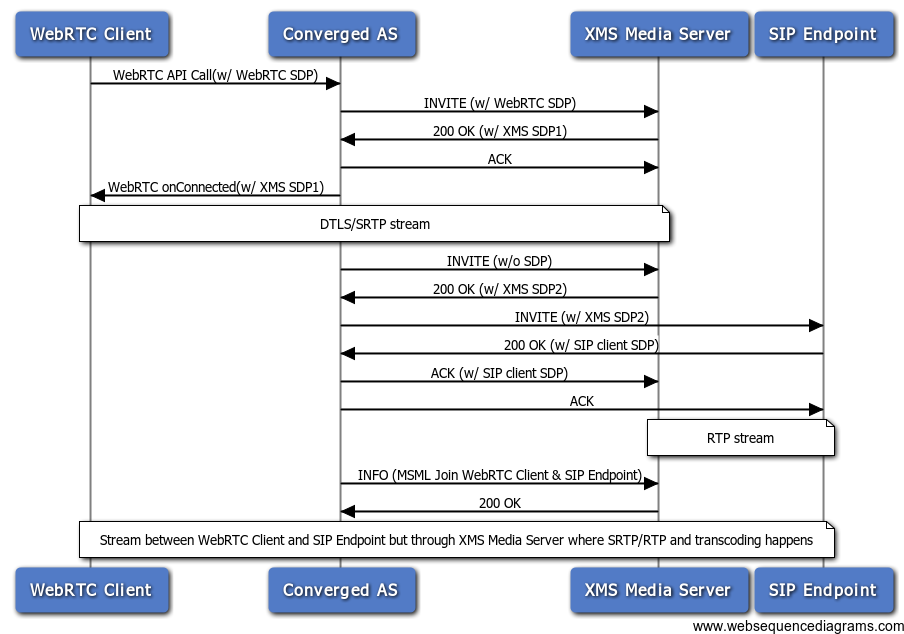
\includegraphics[width=0.95\textwidth,natwidth=610,natheight=642]{figs/chrome2xms.png}
  	\caption{Single Call from Browser to SIP Client}
  	\label{fig:chrome2xms}
\end{figure}

\par According to the documentation provided by Dialogic on XMS 2.1 \gls{rest}ful \gls{api}\cite{doc:xms_webapi}, it is only necessary to set \textit{encryption} field as \textit{dtls} and \textit{ice} as field \textit{yes} in the \gls{sdp} for \gls{webrtc} \gls{sdp} otherwise not set both fields for \gls{sip} \gls{sdp} when creating a call resource on XMS media server(shown at line 4 and 5 in Code Snippet \ref{code:xms}). It makes the interfaces on application server not necessarily be implemented differently for \gls{webrtc} and \gls{sip} clients.

\par In this sense, there are \textit{createXMSCall()}, \textit{joinXMSCall()}, \textit{updateLocalSDP()}, \textit{createConference()}, \textit{joinConference()}, \textit{deleteXMSCall()} and \textit{deleteXMSConference()} interfaces(shown in Code Snippet \ref{code:xms} ) implemented on application server by the reference of XMS 2.1 RESTful API User's Guide \cite{doc:xms_webapi}.

\par Using \textit{createXMSCall()} function as example of XMS integration implementation (from line 1 to line 37 in Code Snippet \ref{code:xms}), application server uses \textit{http} Node.js module and \textit{xml2js} Node.js module to implement this interface. Regards to XMS 2.1 \gls{rest}ful \gls{api}, creating call resource on XMS media server is a \textit{POST} \gls{http} request with configuration \gls{xml} as request content. From line 2 to line 7 n Code Snippet \ref{code:xms} is to generate the \gls{xml} content. And at line 8, application server calls \textit{http.request()} function with the \textit{option} object and callback function as arguments. The request \textit{option} object has \textit{host},\textit{port},\textit{method},\textit{path},\textit{headers} fields need to be set. The important point is that the \textit{Content-length} is necessary in the headers field, it is the length of the \gls{xml} content. These configuration is implemented from line 9 to line 17 in Code Snippet \ref{code:xms}. At line 35, application server calls \textit{req.write()} function to write \gls{xml} content data in \gls{http} request and sends it to XMS media server. There is a callback function along with the asynchronous function (\textit{http.request()}). In the callback function, application server needs to check the response data from the \gls{http} \textit{POST} request for useful \gls{sdp} data. By using \textit{xml2js} module object \textit{xmlparser} to parse the \gls{xml} data into \gls{json}, at line 26 and line 27, it is the process to strip the useful data \gls{sdp} from the response data. It is easier to keep using \gls{json} format for all the data object in Node.js as well as the application client. After the other process at line 28 and line 30, replacing some unsupported character in the \gls{sdp} for XMS media server by \textit{string.replace()} function, the \textit{createXMSCall()} function will return usful \gls{sdp} as result.

\begin{figure}
	\centering
    	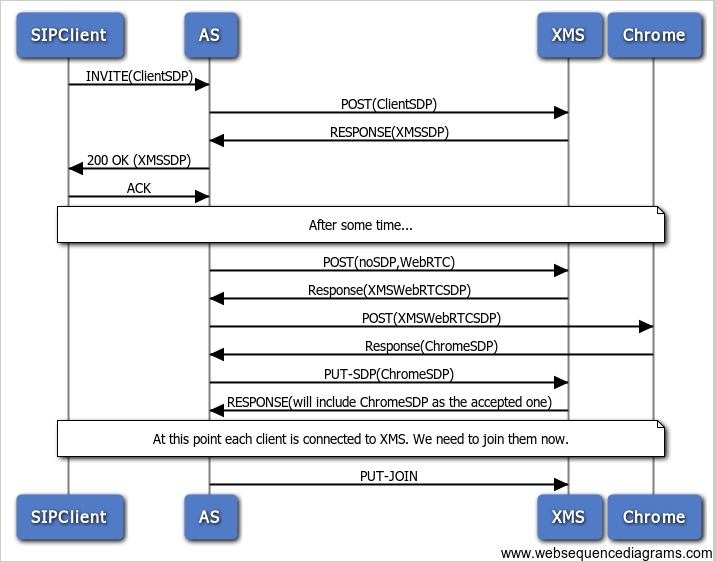
\includegraphics[width=0.95\textwidth,natwidth=610,natheight=642]{figs/sip2xms.png}
  	\caption{Single Call from SIP Client to Browser Client}
  	\label{fig:sip2xms}
\end{figure}

\par The rest of the interfaces for XMS media server on application server are similar with \textit{createXMSCall()} interface. \textit{joinXMSCall()} interface is made for single call resource join with another single call resource, it is used when a \gls{webrtc} call resource join a \gls{sip} call resource for single pair conversation in the prototype system. \textit{updateLocalSDP()} is made to update the \gls{sdp} of specific call resource on the XMS media server, but it does not work well against the current XMS media server when the \gls{webrtc} call resource is made without \gls{sdp} during the test and development. For this reason, the prototype application server can not use the normal process shown in Figure \ref{fig:sip2xms} when application server got a \gls{sip} \textit{INVITE} message. During the test, after creating the \gls{webrtc} call resource on XMS media server without \gls{sdp} and updating it later with the browser client answer \gls{sdp}, browser client fails to connect with the call resource on XMS media server in the \gls{rtp} session. To fix that, the application does the same process for the \gls{webrtc} part as the process shown in Figure \ref{fig:chrome2xms}. It means that no matter the \gls{webrtc} client is a receiver or a sender of the call request during the establishment, for \gls{webrtc} client itself will treat itself as a sender all the time, then the application server can always get the correct \gls{sdp} from the client to create the \gls{webrtc} call resource on XMS media server. This implementation of fixing solution is based on the WebSocket channels \textit{answer} and \textit{answerInvite} for both client side and server side Soket.IO code blocks with the \textit{self} flag value to see if the client is sender or receiver of the \textit{INVITE} message. This issue is reported to Dialogic team, hope it will be resolved in the future version of XMS media server.

\par \textit{createConference()} and \textit{joinConference()} are the corresponding interfaces against \textit{createXMSCall()} and \textit{joinXMSCall()}, they are made for conference resources usage on XMS media server. \textit{deleteXMSCall()} and \textit{deleteXMSConference()} are the delete functions for call resources and conference resources on XMS media server.

\section{Advanced Communication Function Implementation}

\noindent The most exciting reason for combining \gls{webrtc} technology with \gls{sip} \gls{voip} network is that there will be more advanced communication functions can be implemented under the power of web technology. There are two main advanced communication functions implemented in the prototype system.

\subsection{SMS Messaging}

\par \gls{sms} messaging is required for normal telephone usage. In the prototype system, it is necessary to have \gls{sms} messaging function during the conference if one of the participants is on his mobile phone only. The working prototype is shown in Figure \ref{fig:webgui_join_conference}. There are two peers in one conference, two of them are \gls{webrtc} clients(Gintel tester1, Gintel tester2) and one mobile phone client(Brian Chen). The implementation service is based on \gls{msg} provided by Gintel AS. It is a message service gateway for \gls{sip} clients to send \gls{sms} to other \gls{sip} clients or physical mobile phone. The implementation is shown in Code Snippet \ref{code:msg}. It uses the same \gls{http} Node.js module to implement the \gls{http} request communication with \gls{msg} server.

\begin{figure}
	\centering
    	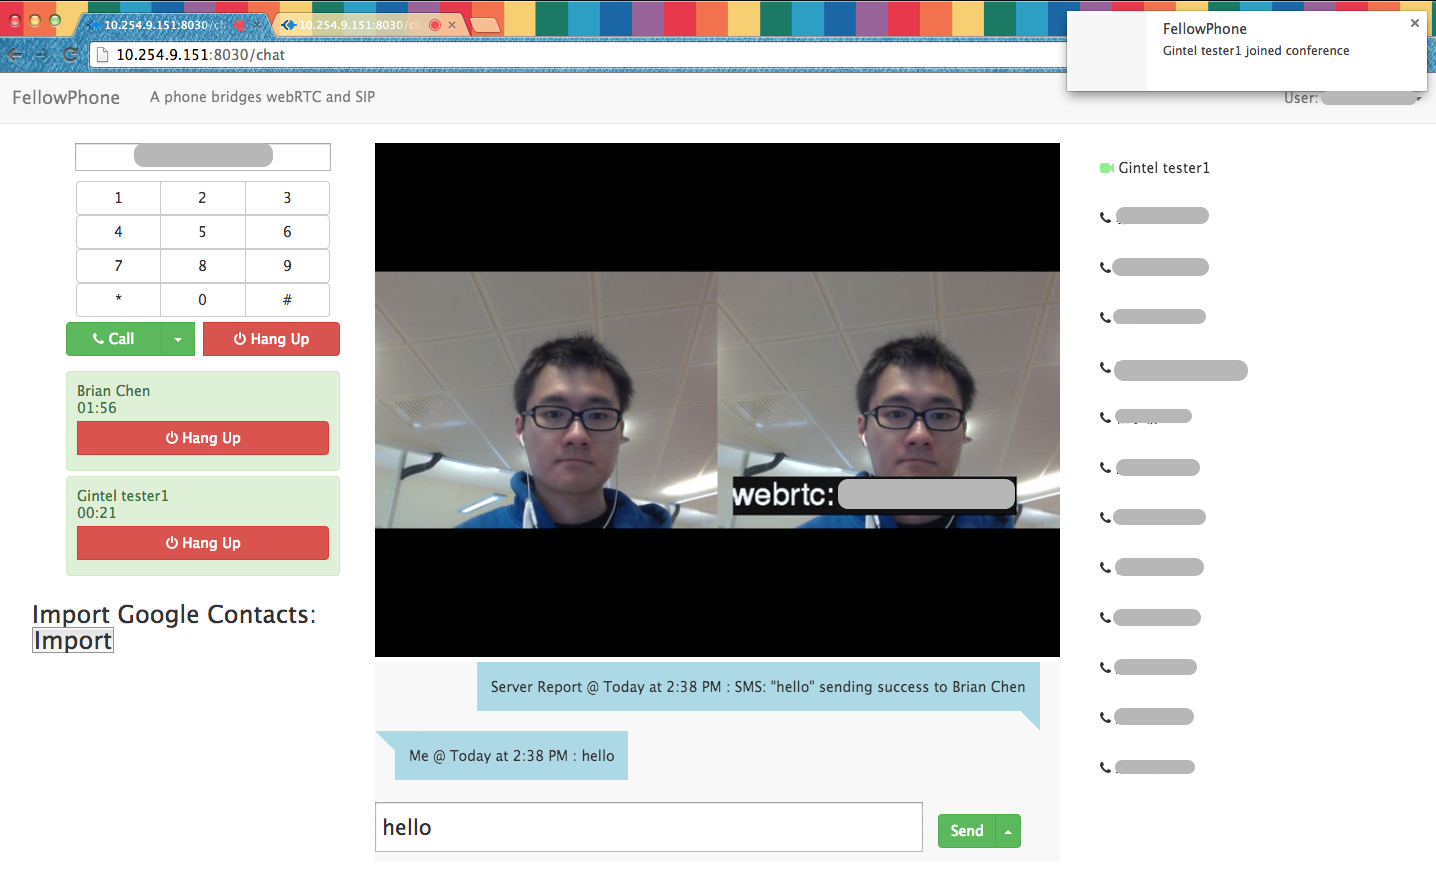
\includegraphics[width=0.95\textwidth,natwidth=610,natheight=642]{figs/webgui_join_conference.png}
  	\caption{Prototype Application in Conference Sending SMS}
  	\label{fig:webgui_join_conference}
\end{figure}

\par There are two steps to send \gls{sms} message. The first one is to get correct \gls{msg} user credential by providing the correct \textit{loginDto} object. \textit{loginDto} is a \gls{json} object generated with the user name and password. From line 2 to line 23 in Code Snippet \ref{code:msg} is the implementation of this process. It uses another Node.js framework library \textit{https.request()} function because of \gls{https} protocol is used on target \gls{msg}. This library can be used in the same pattern as \textit{http.request()} described before. However, \textit{https.request} takes only string text in the header fields, then at line 2 in Code Snippet \ref{code:msg}, it converts \gls{json} object into string. At line 13 in Code Snippet \ref{code:msg}, it is shown that if the credential sent to \gls{msg} server is correct, it will return a validate cookie in response data. This cookie will be used for second step to send \gls{sms} message. From line 25 to line 61 is the implementation of second step, the login credential and cookie need to be set in the header fields \textit{login} and \textit{Cookie}(shown at line 23 and 36). Moreover the message string is set in the \gls{http} request body at line 59, the \textit{Content-Type} and \textit{Content-Length} in the headers should be set as "application/json" and the length of message string content(it shows at line 33 and line 37).

\subsection{Files Sharing}

\par Because the \gls{rtp} media channel is connected with XMS media server for media  stream exchange, \gls{webrtc} \textit{RTCDataChannel} can not be used in this case. However, considering the prototype system is a real-time communication platform for collaboration working scenario, it is necessary for end points to have some collaboration tools such as files sharing. The screen shoot of file sharing in prototype application is shown in Figure \ref{fig:webgui_file_share_sender} and Figure \ref{fig:webgui_file_share_receiver}.

\begin{figure}
	\centering
    	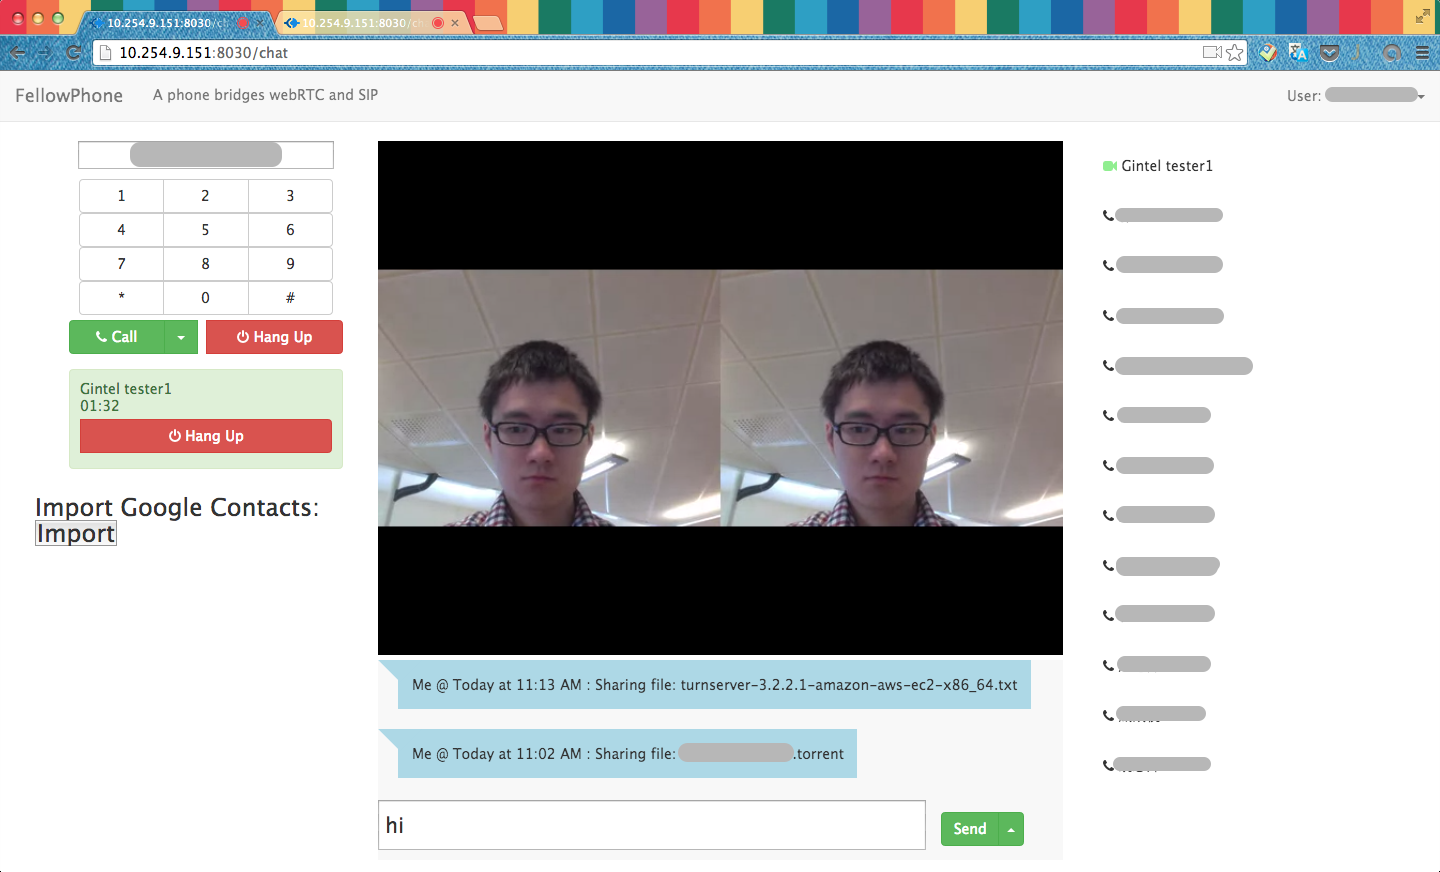
\includegraphics[width=0.85\textwidth,natwidth=610,natheight=642]{figs/webgui_file_share_sender.png}
  	\caption{File Sharing Sender Client}
  	\label{fig:webgui_file_share_sender}
  	    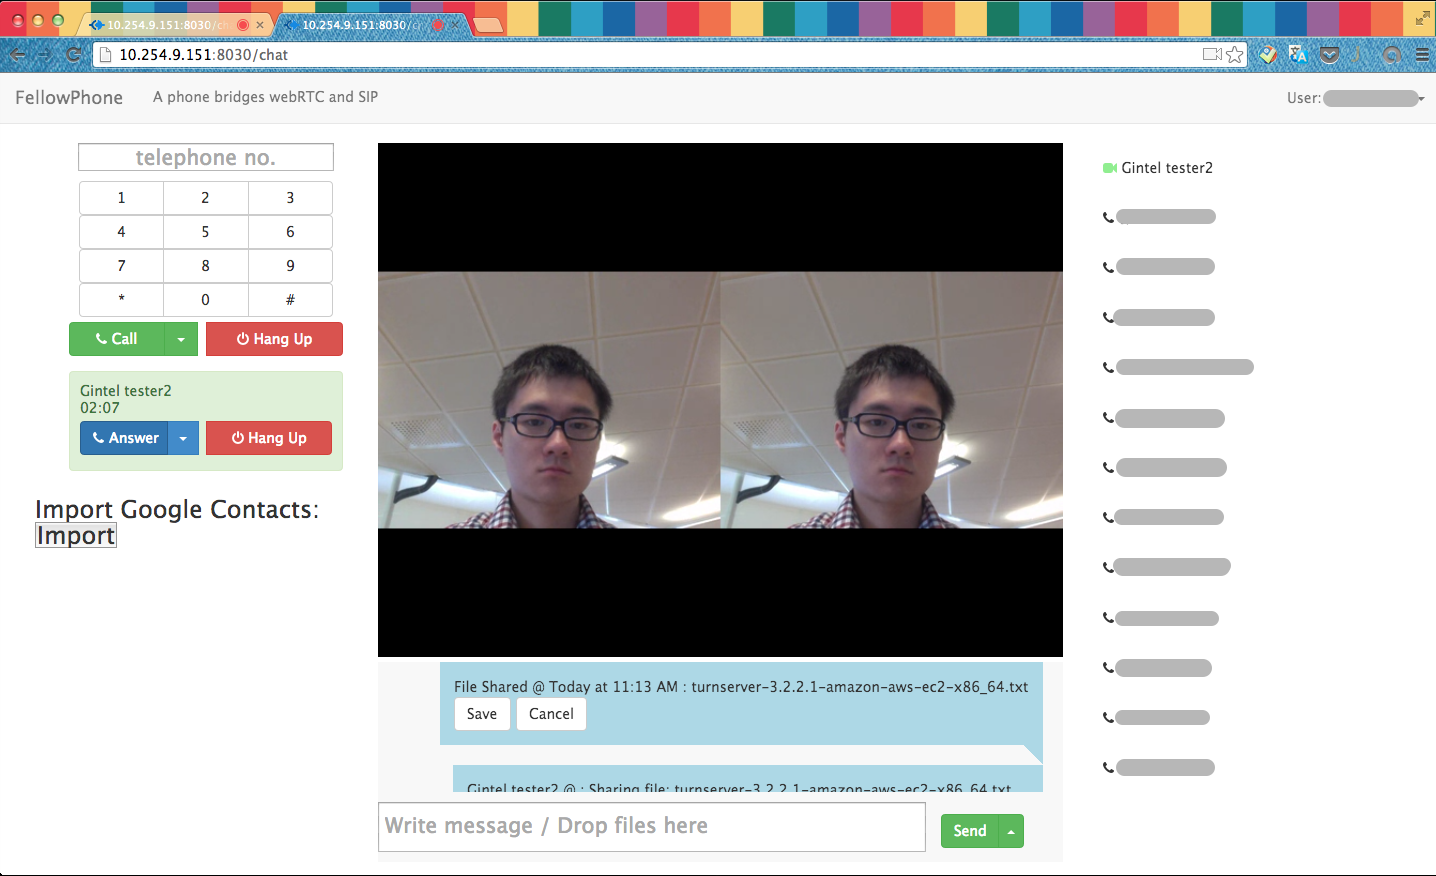
\includegraphics[width=0.85\textwidth,natwidth=610,natheight=642]{figs/webgui_file_share_receiver.png}
  	\caption{File Sharing Receiver Client}
  	\label{fig:webgui_file_share_receiver}
\end{figure}

\par As the screen shoot showing, when sender client uploads files to the application server, application server will directly share these files with the other clients in current conference session. The receiver client can decide whether these files need to be saved or not.

\par Prototype application uses Delivery.js library to do bidirectional File Transfers For Node.js via Socket.IO. Delivery.js uses Node.js and Socket.IO to make it easy to push files to the client, or send them to the server. Files can be pushed to the client as text (utf-8) or base64 (for images and binary files).\cite{github:deliveryjs} Since it is based on Socket.IO, it has the similar client and server implementation mechanism as Socket.IO. Once a WebSocket connection is established messages (frames) sent between the client and server contain only 2 additional bytes of overhead. In contrast, a traditional \textit{POST} request, and response, may have headers totaling 871 bytes. This could be a significant addition if many files are being sent, and would be even more significant if files are being divided into batches before being sent to the server. When pushing files to the client, the overhead of traditional polling methods provides an even starker contrast to WebSockets.

\par At line 9 in Code Snippet \ref{code:server_socket}, it declares the \textit{delivery} object using Delivery.js \gls{api} \textit{dl.listen()} with the Socket.IO \textit{socket} object as the argument. From line 36 to line 64 in Code Snippet \ref{code:server_socket} is the server side Delivery.js implementation code. It listens to the 'receive.success' WebSocket channel, when the upload files from client are received successfully the application server will make temporary files for the upload files and push these files to every connected clients in sender's current conference session. At line 38, application server uses \textit{fs.writeFile()} function from the Node.js framework \textit{fs} library to write the file byte data got from the client to the application server file system, then at line 46, it uses Delivery.js \textit{delivery.send()} function to push the file to the connected WebScoket client. For security reasons, the temporary files will be removed from the server when all the pushing process finished, it is implemented at line 54 by using \textit{fs.unlink()} function from Node.js framework \textit{fs} library.

\par After the files are pushed to the client, at line 42 in Code Snippet \ref{code:chatboard_ctrl}, the client side implementation will listen to the same WebSocket channel 'receive.success'. When there is file message from the application server to the client, the client listener will save the files in the runtime memory (it is not best solution for files sharing case, the improvement will be discussed in Chapter \ref{chp:future_work}), then let the user decide if these files need to be downloaded or removed. At line 32 in Code Snippet \ref{code:chatboard_ctrl}, it is the client side sending files function (\textit{delivery.send()}) to the server through WebSocket.

\begin{lstlisting}[caption={Files Sharing in ChatBoardCtrl.js},label={code:chatboard_ctrl}]
angular.module('webrtcDemo.controllers').
	controller('ChatBoardCtrl',function ($scope,$location,$upload,WebSocketService,storage,appId) {
		...
		function b64toBlob(b64Data, contentType, sliceSize) {
	    contentType = contentType || '';
	    sliceSize = sliceSize || 512;

	    var byteCharacters = atob(b64Data);
	    var byteArrays = [];

	    for (var offset = 0; offset < byteCharacters.length; offset += sliceSize) {
	        var slice = byteCharacters.slice(offset, offset + sliceSize);

	        var byteNumbers = new Array(slice.length);
	        for (var i = 0; i < slice.length; i++) {
	            byteNumbers[i] = slice.charCodeAt(i);
	        }

	        var byteArray = new Uint8Array(byteNumbers);

	        byteArrays.push(byteArray);
	    }

	    var blob = new Blob(byteArrays, {type: contentType});
	    return blob;
		}
        ...
		function _upload(files){
  		if(channelReday){
  			_.each(files,function(file){
  				...
					delivery.send(file);
  			});
  		}
  	}
  	...
		function _initChatBoardView(){
			socket = WebSocketService.getCurrentSocket();
			...
			delivery = new Delivery(socket);
			...
			delivery.on('receive.success',function(file){
	          $scope.recievedFiles.push(file);
	          ...	    
	      });
			...
		}
		...
  	$scope.saveFile = function(msg,filename){
  		var tempFile = _.find($scope.recievedFiles,function(file){
				return file.name == filename;
			});

  		var fileBlob = b64toBlob(tempFile.data,tempFile.mimeType);
  		saveAs(fileBlob, tempFile.name);
  		...
  	}
  	...
  });
\end{lstlisting}


\par Because Delivery.js sends files in base64\footnote{Base64 is a group of similar binary-to-text encoding schemes that represent binary data in an ASCII string format by translating it into a radix-64 representation. The term Base64 originates from a specific MIME content transfer encoding.\cite{wiki:base64}} encoding format, on the client application, it is necessary to convert base64 encoding string to Web \textit{Blob}\footnote{A Blob object represents a file-like object of immutable, raw data. Blobs represent data that isn't necessarily in a JavaScript-native format. The File interface is based on Blob, inheriting blob functionality and expanding it to support files on the user's system.\cite{mdn:blob}} data for using the \gls{html5} \gls{w3c} \textit{saveAs()} function to download file at line 55 in Code Snippet \ref{code:chatboard_ctrl}. The \textit{saveAs()} function takes Web \textit{Blob} object and file name as the two function parameters. The converting function is implemented at line 4 to line 26 as \textit{b64toBlob()} function in Code Snippet \ref{code:chatboard_ctrl}, it takes base64 string, content type of the file and slice size (in the prototype case it uses default 512 bit) to convert base64 string data to Web \textit{Blob} data. The important function in this code block is \textit{atob()}, it decodes a string of data which has been encoded using base-64 encoding, then slice the byte character data into byte array since \textit{Blob()} function only takes array of data objects, shown at line 24.

\par Based on these implementation for file sharing, it is even possible to send an E-mail with the sharing files as attachments to the current mobile phone(\gls{sip} client) participant in the conference on the application server. Although the mobile phone (\gls{sip} client) can not get the sharing files directly in real time, the user can still browser these shared files during the conference to discuss the topic with other participants.


\chapter{Prototype System Deployment}
\label{chp:sys_deploy}

\noindent In this Chapter, there will be three main topics discussed because of deploying the prototype system to production usage.

\section{TURN Server Deployment}

\par During the development of the prototype system, the test based on XMS media server is not stable at the beginning. There is one way audio issue happens in the prototype system when \gls{webrtc} client init a outbound call to a \gls{sip} client(mobile phone). Since it is working fine when the outbound \gls{sip} client call into the \gls{webrtc} client, after tracing the network log from the XMS media server, the problem is the \gls{ice} candidate information got from the original \gls{stun} server can not punch the whole on the firewall of the XMS media server. It is normal to replace the \gls{stun} server as \gls{turn} server to solve this problem because if the \gls{stun} server way is blocked during the media stream exchange from two end point, it will switch to \gls{turn} server way to exchange the media stream through the \gls{turn} server to rely all the media traffic.

\par Moreover, the \gls{turn} server solution will work well in the different corporation networks scenario since there will be highly restrict corporation firewall in front of the corporation network. Then \gls{turn} server can rely all the media stream to establish the peer to peer connection. After testing prototype system against \gls{turn} server instead of \gls{stun} server provided by Google (shown at line 3 in Code Snippet \ref{code:create_peer_connection}), the one way audio issue is solved and two end client in different corporation network scenario works fine as well.

\par To set up \gls{turn} server in the production of prototype system, the prototype system uses \gls{aws} \gls{ec2}\footnote{Amazon Elastic Compute Cloud (EC2) is a central part of Amazon.com's cloud computing platform, Amazon Web Services (AWS). EC2 allows users to rent virtual computers on which to run their own computer applications. EC2 allows scalable deployment of applications by providing a Web service through which a user can boot an Amazon Machine Image to create a virtual machine, which Amazon calls an "instance", containing any software desired. A user can create, launch, and terminate server instances as needed, paying by the hour for active servers, hence the term "elastic". EC2 provides users with control over the geographical location of instances that allows for latency optimization and high levels of redundancy.\cite{wiki:ec2}}, \gls{ip} address: 54.187.157.224. There is a free open source implementation of \gls{turn} and \gls{stun} server maintained by Google. It provides the \gls{aws} \gls{ec2} hosting image, then it is only necessary to configure the \gls{aws} \gls{ec2} virtual instance to open the necessary ports for the \gls{turn} server usage. It is shown in the following list:
\begin{itemize}[topsep=-1em,parsep=0em,itemsep=0em]
 \item TCP 443
 \item TCP 3478-3479
 \item TCP 32355-65535
 \item UDP 3478-3479
 \item UDP 32355-65535
\end{itemize}

\par Moreover, the \gls{turn} server can either use a flat file or a \gls{sql} database for configuration and user information. In the prototype system, the \gls{turn} server on \gls{aws} \gls{ec2} will use a flat file for configuration and user information. It is edited in "/usr/local/etc/turnuserdb.conf" by adding an entry on its own line: "my\_username:my\_password".\cite{dialogic:turn} Other configurations need to be completed by following the README file under the hosting instance image directory on \gls{aws} \gls{ec2}. There are several paramters need to be set in "/etc/turnserver.conf" on \gls{turn} server.

\par Besides establishment for \gls{turn} server, there are some changes need to be done on the client application as well in order to use this \gls{turn} server to fetch the useful \gls{ice} candidate information during the peer to peer connection. Compare to the Code Snippet \ref{code:create_peer_connection} with original Google \gls{stun} server address, in Code Snippet \ref{code:client_turn_server}, prototype \gls{turn} server is set as \textit{iceServer}. The \textit{iceTransports} field is the parameter to force client to use \gls{turn} server but it is only purposed by Google Chrome, it is not standard and it is not implemented in Google Chrome yet.

\begin{lstlisting}[caption={Using TURN Server on WebRTC Client},label={code:client_turn_server}]
if (location.hostname != "localhost") {
  			
				pc_config = 
				{
					'iceServers': [{
						'urls': 'turn:54.187.157.224',
						'username': 'my_username',
						'credential': 'my_password'
					}],
					'iceTransports': 'relay'
				};
			}
\end{lstlisting}


\section{Application Server Deployment}

\par Because the prototype application server is implemented in Node.js, there is no restrict requirements for the operation system platform to deploy the application server if the operation system can install Node.js library and can run V8 JavaScript Engine\footnote{The V8 JavaScript Engine is an open source JavaScript engine developed by Google for the Google Chrome web browser.V8 compiles JavaScript to native machine code (IA-32, x86-64, ARM, or MIPS ISAs) before executing it, instead of more traditional techniques such as interpreting bytecode or compiling whole program to machine code and executing it from a filesystem. \cite{wiki:v8}}.

\par It also needs to open the \textit{5060} port to support \gls{udp} for \gls{sip} stack usage. Then it just need to use \textit{node server.js} command to host the application server for production.

\section{XMS Server Deployment}

\par The XMS media server is host on a stand alone machine during the development. For deployment reason, it is necessary to map the internal \gls{ip} address of XMS media server to a public \gls{ip} address. And it is important to open the necessary port for the XMS media usage. According to the documentation of Dialogic PowerMedia XMS 
Installation and Configuration Guide\cite{dialogic:xms_install},the default PowerMedia XMS configuration uses the following ports:
\begin{itemize}[topsep=-1em,parsep=0em,itemsep=0em]
 \item \gls{tcp}: 22, 80, 81, 443, 5060, 1080, 15001 
 \item \gls{udp}: 5060, 49152-53152, 57344-57840 
\end{itemize}

\par Because the application server and XMS media server in the prototype system are host in the corporation network, it only opens necessary port to the public network. During the exchange \gls{ice} candidate information for client, the XMS \gls{ip} address will be the internal \gls{ip} address by the rule of the corporation network. It is necessary to change the internal \gls{ip} address into public \gls{ip} address before pushing the \gls{ice} candidate information back to the end point client. This process is implemented at line 29 in Code Snippet \ref{code:xms}, it simply just replaces the internal \gls{ip} address as public \gls{ip} address of XMS media server in the \gls{sdp} content string.


\chapter{Discussion and Conclusion}
\label{chp:future_work}

\noindent In this Chapter, there are some future improvements discussion for the prototype system will be discussed. And some future research directions of \gls{webrtc} integrated with traditional telephony network will be include as well.

\section{Future Work}

\subsection{RTCDataChannel usage}

\par The \textit{RTCDataChannel} \gls{api} enables peer-to-peer exchange of arbitrary data, with low latency and high throughput.The API has several features to make the most of \textit{RTCPeerConnection} and enable powerful and flexible peer-to-peer communication\cite{html5rock:webrtc}:

\begin{itemize}[topsep=-1em,parsep=0em,itemsep=0em]
    \item Leveraging of RTCPeerConnection session setup.
    \item Multiple simultaneous channels, with prioritization.
    \item Reliable and unreliable delivery semantics.
    \item Built-in security (\gls{dtls}) and congestion control.
    \item Ability to use with or without audio or video.
\end{itemize}

\par Communication occurs directly between browsers, so RTCDataChannel can be much faster than WebSocket even if a relay (\gls{turn}) server is required when 'hole punching' to cope with firewalls and \gls{nat}s fails.

\par Because the XMS media server handles all the media stream exchange between the end point clients and it is not support \textit{RTCDataChannel}, the prototype application does not implement \textit{RTCDataChannel} feature in the system. Current using Delivery.js library is good at bidirectional file sharing between clients and server through WebSocket. But it has some disadvantages still. The most apparent disadvantage would be the fact that it bypasses traditional caching methods. Instead of caching based on a file’s URL, caching would be based on the content of the Web Socket’s message. One possibility would be to cache a base64, or text, version of the file within Redis\footnote{Redis is an open-source, networked, in-memory, key-value data store with optional durability. It is written in ANSI C.\cite{wiki:redis}} for fast, in memory, access. And also the sharing files are uploaded to the server then pushing back to the other clients, it takes longer time to finish this process than peer-to-peer sharing files. Moreover, in current prototype system, the shared files will be temporary pre-stored for the client, it will cause some problem when the sharing file is in a very big size and it will take over all the memory resource which the client has.

\par One obvious solution will be implementing the \textit{RTCDataChannel} \gls{api} on each connected client and create new \textit{RTCPeerConnection} for each pair user in mesh network for only sharing files purpose. Since these new \textit{RTCPeerConnection}
is not necessary active during the whole time of application using, they are possible to be removed after they are used for sharing files to release more memory recourse for browser clients.

\par The other solution will be using third party peer to peer sharing services, such as Sharefest\footnote{One-To-Many sharing application. Serverless. Eliminates the need to fully upload your file to services such as Dropbox or Google Drive. Put your file and start sharing immediately with anyone that enters the page. Pure javascript-based. No plugins needed thanks to HTML5 WebRTC Data Channel API}. It operates on a mesh network similar to Bit-torrent network. The main difference is that currently the peers are coordinated using an intelligent server. This coordinator controls which parts are sent from A to B and who shall talk with whom. Peer5(\url{http://peer5.com/}) Coordinator (or any other solution) is used to accomplish this. Each peer will connect to few other peers in order to maximize the distribution of the file.\cite{github:sharefest} In this case the client will still keep having single \textit{RTCPeerConnection} with the \textit{RTCDataChannel} on the client, it will fit the work scenario of the prototype system.

\subsection{Browser Compatibility}

\par The prototype system is developed on a single browser (Google Chrome), it is not tested on other browser. The main reason is that the bug fixing for cross browser platform on \gls{webrtc} is too complicated and changed a lot during the development. Since \gls{webrtc} is not standard Web \gls{api} yet, all the browsers have their own implementation. Although most of the \gls{webrtc} \gls{api}s used in the application layer are more or less the same, the issues happen in different ways and they are hard to debug.

\par Fortunately, Google provides the \textit{adapter.js} script for developers to solve the cross platform issue on Google Chrome and Firefox. It is implemented in WebRTCService in prototype application client. During the test, it still happens some compatibility issues between Google Chrome and Firefox. Current version of prototype system is working fine on both Google Chrome and Firefox browser. However, there are some problem when call is made from Firefox to Google Chrome, from Google Chrome to Firefox works. The main reason for that, it is the \gls{sdp} content generated on both platform is not compatible in this work scenario. This issue need to be fixed in the future work.

\subsection{Media Server Performance}

\par During the test of the prototype system, the XMS media server performance is quite concerned in the work scenario. The main reason is that the current XMS media server host on a normal laptop machine, it is not powerful enough for high traffic load of the media stream exchange.

\par The solution for that, it would be easy to host the media server on another powerful server machine. Considering the purpose of the prototype system is to build a system integrated with \gls{webrtc} and \gls{voip} network, it is not good solution to keep updating the XMS media server machine. There will be two way to solve this issue in real time communication work scenario. One is to host XMS media server on the third party cloud service, like \gls{aws} \gls{ec2} instance. Because the third party service will handle the machine performance, it will rarely have the problem on machine performance issue. However, this solution is quite expensive when huge number of users make large amount of media stream traffic to the XMS media server. The other solution will be distribute multiple XMS media server to share the traffic load in the prototype system. Then it will be easy to control the performance of the media server but it will cost more physical machine expense.

\par As a result, the performance of the media server need to be considered as the cost of media server deployment and distribution together.

\subsection{Object RTC (ORTC) API for WebRTC}

\par \gls{ortc} is a free, open project that enables mobile endpoints to talk to servers and web browsers with \gls{rtc} capabilities via native and simple Javascript APIs. The Object RTC components are being optimized to best serve this purpose.\cite{website:ortc} The mission of \gls{ortc} is to enable rich, high quality, RTC applications to be developed in mobile endpoints and servers via native toolkits, simple Javascript APIs and HTML5. It is also a mandate that Object RTC be compatible with WebRTC.

\par Current WebRTC client is made for browser only, only the smart phone with supported mobile web browser can use these application. According to \gls{ortc}, it is possible to make all the smart phone as a \gls{webrtc} client. Then there will be no more different signaling implementation because both end point use \gls{webrtc} \gls{sdp} content and \gls{webrtc} mechanism. Only one signaling mechanism need to be implemented in this way, it will make less compatibility problem for different types end points.

\par There is a related open source project, ortc-lib (\url{https://github.com/openpeer/ortc-lib}), it is \gls{ortc} C++ library wrapper for \gls{webrtc}.This \gls{sdk} library implementation of the \gls{ortc} specification that will enable mobile end points to talk to a \gls{webrtc} enabled browser.

\par If we look at the success of apps like Whatsapp\footnote{WhatsApp Messenger is a proprietary, cross-platform instant messaging subscription service for smartphones that uses the internet for communication. In addition to text messaging, users can send each other images, video, and audio media messages as well as their location using integrated mapping features.} , Tango\footnote{Tango is third-party, cross platform messaging application software for smartphones developed by TangoME, Inc.} , Viber\footnote{Viber is a proprietary cross-platform instant messaging voice-over-Internet Protocol application for smartphones developed by Viber Media.}, Voxer\footnote{Voxer is a San Francisco based mobile app development company most well known for its free Voxer Walkie Talkie app for smartphones.}, Facebook Messenger\footnote{Facebook Messenger is an instant messaging service and software application which provides text and voice communication. Integrated with Facebook's web-based Chat feature and built on the open MQTT protocol,Messenger lets Facebook users chat with friends both on mobile and on the main website.} etc these are all \gls{ott} applications that have already won in mobile communications. Placing a phone call, is nearly the last thing a teen or twenty-something user is looking to do with their phone nowadays.\cite{web:ott_com} If the concept of \gls{ortc} has been widely spread and implemented, \gls{webrtc} and \gls{ortc} will become the next generation telecommunication network.

\subsection{Advanced function for telecommunication}

\par Since the prototype system bridges the web network and telecommunication network, it is easy to think about how to implement powerful web technology with the telephony use case. For example real time translation in speaking. Translator.js is a JavaScript library built on top of Google Speech-Recognition \& Translation API to transcript and translate voice and text. It supports many locales and brings globalization in \gls{webrtc}.\cite{github:translatorjs} It uses Google Speech-Recognition \gls{api} to convert user spoken sentence into text string, then uses Google's Non-Official Translation \gls{api} to translate the text into target language text and use \textit{meSpeak.js} library to play text using a robot voice.

\par With the social network information, it is easy to get the person profile information of the current conversation user. It is possible to visualize the social network topological diagram to show what is the relationship between two speaking user in the conversation. For the business conference using, it is possible to know the person information and company background information during the conference.

\par Furthermore, with the voice recognization on the web, it is possible to make any useful command through the video/audio conference. For example, one of users want other people to send an E-mail with some attachments to him and mentioned it during the conversation. Then the other user's application will recognize the command and generate the E-mail content at the same time and add the files from the computer as attachments. It will make the normal conference meeting more efficient and less misunderstanding and better for reminding.

\section{Conclusion}

\par Considering about the research of this thesis and the prototype system, it is clearly that the unified communication service with \gls{webrtc} is a promising concept in the telecommunication industry. The functions provided by prototype system will rich the traditional telephony service for users. The objective of this thesis is achieved by the prototype system, the prototype system can provide an unified communication service based on \gls{webrtc} and \gls{sip}.

\par The advantage of prototype system is that it does not require users to install any application client and it is no need for users to have another user credential for this service (prototype system uses telephone number as user credential). Moreover, this unified communication service is server centralized system, it will have more advanced real time communication functions can be implemented on both server side and client side. In this system architecture, there is more space for developers to add more advanced functions and it is easier for scaling for larger user base.

\par Because the prototype system is based on \gls{webrtc}, it means that it is highly dependent on web browser client. More advanced concept about unified communication service would be implementing \gls{ott} real time communication. It will either require the mobile browsers on the smart phones implemented for \gls{webrtc} standard or \gls{webrtc} can be implemented on different mobile operation platform as native \gls{api}. Afterwards, there will be more devices can use prototype system to have rich real time communication service between mobile phone users and computer users. Therefore, current application client of the prototype system is based on browser client. The compatible devices which can use the application client are \gls{webrtc} supported browsers. Because there are not so many mobile browsers support \gls{webrtc} yet, then the user clients to use the prototype application are computer clients only, there are more potential users on the mobile platform.

\par The performance of the prototype system needs to be concerned in the future work because it is hard to evaluate the performance under small group of users and poor server machines. Although the prototype system is not production project, it is still deployed on the public network to test the network issues on the real working scenario. The reason of this thesis implemented prototype system deployment is because there are many feedback about network firewall issues mentioned in other \gls{webrtc} web service. It is critical to test the deployment of the prototype system to avoid later big changes for the network architecture because the network problem. The result of the prototype system deployment is verified that the prototype network architecture is a good solution in the working scenario.

\par Furthermore, there is no commercial products to provide unified communication service based on \gls{webrtc} and \gls{sip}. There are many potential usage of the prototype system integrated with other popular web service in different industry area. And the bridge to connect the web world and telephony work is the prototype system service. The unified communication service will be the big game changing for the web communication and telephony communication business.


\renewcommand*{\bibname}{References}
\nocite{*}
\bibliographystyle{alpha}
\bibliography{main}

\appendix
\addtocontents{toc}{%
  \protect\vspace{1em}% 
  \protect\noindent \bfseries \appendixtocname\protect\par
  \protect\vspace{-.5em}%
 }
 \renewcommand{\chaptername}{\appendixname}
 
\begin{appendices}

\chapter{Appendix A}

\section{WebRTCService} \label{app:webrtc_service}

\begin{lstlisting}[caption={WebRTCService in application client},label={code:webrtc_service}]
'use strict';

/**
*  services Module
*
* WebRTCService with browser adapter.js function
*/

angular.module('webrtcDemo.services').
	factory('WebRTCService',function () {
		var _ws;//websocket obj
		
		var _RTCPeerConnection;
		var _RTCSessionDescription;
		var _RTCIceCandidate;
		var _getUserMedia;
		var _createIceServer;
		var _attachMediaStream;
		var _reattachMediaStream;
		var _webrtcDetectedBrowser;
		var _webrtcDetectedVersion;

		function _initWebRTC () {
			_RTCPeerConnection = null;
			_RTCSessionDescription = null;
			_RTCIceCandidate = null;
			_getUserMedia = null;
			_createIceServer = null;
			_attachMediaStream = null;
			_reattachMediaStream = null;
			_webrtcDetectedBrowser = null;
			_webrtcDetectedVersion = null;

			_setRTCElement();
		}

		function _setRTCElement() {

			if(navigator.mozGetUserMedia){
				console.log("This appears to be Firefox");

				_webrtcDetectedBrowser = "firefox";
				_webrtcDetectedVersion = parseInt(navigator.userAgent.match(/Firefox\/([0-9]+)\./)[1], 10);

				_RTCPeerConnection = mozRTCPeerConnection;
				_RTCSessionDescription = mozRTCSessionDescription;
  			_RTCIceCandidate = mozRTCIceCandidate;
  			_getUserMedia = navigator.mozGetUserMedia.bind(navigator);

  			// Creates iceServer from the url for FF.
			  _createIceServer = function(url, username, password) {
			    var iceServer = null;
			    var url_parts = url.split(':');
			    if (url_parts[0].indexOf('stun') === 0) {
			      // Create iceServer with stun url.
			      iceServer = { 'url': url };
			    } else if (url_parts[0].indexOf('turn') === 0) {
			      if (_webrtcDetectedVersion < 27) {
			        // Create iceServer with turn url.
			        // Ignore the transport parameter from TURN url for FF version <=27.
			        var turn_url_parts = url.split("?");
			        // Return null for createIceServer if transport=tcp.
			        if (turn_url_parts.length === 1 ||
			            turn_url_parts[1].indexOf('transport=udp') === 0) {
			          iceServer = { 'url': turn_url_parts[0],
			                        'credential': password,
			                        'username': username };
			        }
			      } else {
			        // FF 27 and above supports transport parameters in TURN url,
			        // So passing in the full url to create iceServer.
			        iceServer = { 'url': url,
			                      'credential': password,
			                      'username': username };
			      }
			    }
			    return iceServer;
			  };

  			_attachMediaStream = function(element, stream) {
			    console.log("Attaching media stream");
			    element.mozSrcObject = stream;
			    element.play();
			  };

			  _reattachMediaStream = function(to, from) {
			    console.log("Reattaching media stream");
			    to.mozSrcObject = from.mozSrcObject;
			    to.play();
			  };

			  // Fake get{Video,Audio}Tracks
			  if (!MediaStream.prototype.getVideoTracks) {
			    MediaStream.prototype.getVideoTracks = function() {
			      return [];
			    };
			  }

			  if (!MediaStream.prototype.getAudioTracks) {
			    MediaStream.prototype.getAudioTracks = function() {
			      return [];
			    };
			  }

			}else if(navigator.webkitGetUserMedia){
				console.log("This appears to be Chrome");

				_webrtcDetectedBrowser = "chrome";
				_webrtcDetectedVersion = parseInt(navigator.userAgent.match(/Chrom(e|ium)\/([0-9]+)\./)[2], 10);

			  _RTCPeerConnection = webkitRTCPeerConnection;
			  _RTCSessionDescription = RTCSessionDescription;
			  _RTCIceCandidate = RTCIceCandidate;
			  _getUserMedia = navigator.webkitGetUserMedia.bind(navigator);

			  // Creates iceServer from the url for Chrome.
			  _createIceServer = function(url, username, password) {
			    var iceServer = null;
			    var url_parts = url.split(':');
			    if (url_parts[0].indexOf('stun') === 0) {
			      // Create iceServer with stun url.
			      iceServer = { 'url': url };
			    } else if (url_parts[0].indexOf('turn') === 0) {
			      if (_webrtcDetectedVersion < 28) {
			        // For pre-M28 chrome versions use old TURN format.
			        var url_turn_parts = url.split("turn:");
			        iceServer = { 'url': 'turn:' + username + '@' + url_turn_parts[1],
			                      'credential': password };
			      } else {
			        // For Chrome M28 & above use new TURN format.
			        iceServer = { 'url': url,
			                      'credential': password,
			                      'username': username };
			      }
			    }
			    return iceServer;
			  };

			  // Attach a media stream to an element.
			  _attachMediaStream = function(element, stream) {
			    if (typeof element.srcObject !== 'undefined') {
			      element.srcObject = stream;
			    } else if (typeof element.mozSrcObject !== 'undefined') {
			      element.mozSrcObject = stream;
			    } else if (typeof element.src !== 'undefined') {
			      element.src = URL.createObjectURL(stream);
			    } else {
			      console.log('Error attaching stream to element.');
			    }
			  };

			  _reattachMediaStream = function(to, from) {
			    to.src = from.src;
			  };

			  // The representation of tracks in a stream is changed in M26
			  // Unify them for earlier Chrome versions in the coexisting period
			  if (!webkitMediaStream.prototype.getVideoTracks) {
			    webkitMediaStream.prototype.getVideoTracks = function() {
			      return this.videoTracks;
			    };
			    webkitMediaStream.prototype.getAudioTracks = function() {
			      return this.audioTracks;
			    };
			  }

			  // New syntax of getXXXStreams method in M26
			  if (!webkitRTCPeerConnection.prototype.getLocalStreams) {
			    webkitRTCPeerConnection.prototype.getLocalStreams = function() {
			      return this.localStreams;
			    };
			    webkitRTCPeerConnection.prototype.getRemoteStreams = function() {
			      return this.remoteStreams;
			    };
			  }

			}else{
				console.log("Browser does not appear to be WebRTC-capable");
			}

		}

		return {
			init : function (socket) {
				if(socket){
					//init service with websocket
					_ws = socket;
				}

				_initWebRTC();

			},

			peerConnection : function(config,constraints){
				if(_RTCPeerConnection){
					return new _RTCPeerConnection(config,constraints);
				}
				return null;
			},

			RTCSessionDescription : function(message){
				if(_RTCSessionDescription){
					return new _RTCSessionDescription(message);
				}
				return null;
			},

			RTCIceCandidate : function(options){
				if(_RTCIceCandidate){
						return new _RTCIceCandidate(options);
					}
					return null;
			},

			webrtcDetectedBrowser : function(){
				return _webrtcDetectedBrowser;
			},

			attachMediaStream : function(element, stream){
				return _attachMediaStream(element, stream);
			},

			reattachMediaStream : function(to, from){
				return _reattachMediaStream(to, from);
			},

			getUserMedia : function(constraints, handleUserMedia, handleUserMediaError){
				return _getUserMedia(constraints, handleUserMedia, handleUserMediaError);
			}

		}
	});	
	
\end{lstlisting}

\end{appendices}

\end{document} 
